\RequirePackage{pdfmanagement-testphase}
\DeclareDocumentMetadata {lang=en-US}

% xmp metadata for pdf
% Originally used \usepackage[a-2a]{pdfx}
% \usepackage{hyperxmp} replaced it
% \RequirePackage{pdfmanagement-testphase} replaced it
% \PassOptionsToPackage{enable-debug,check-declarations}{expl3} broke with version 0.9 of tagpdf
% \ExplSyntaxOn no need for these 3 lines because metadata can handle it
% \pdfmanagement_add:nnn{Catalog}{Lang}{(enUS)} enUS is wrong, should be en-US
% \ExplSyntaxOff

\documentclass[11pt,
  english,
  a4paper,
]{article}
\usepackage{sa4ss}
\usepackage{amsmath,amssymb,array}
\usepackage{booktabs}

% From tagged-template.latex
\usepackage{lmodern}
\usepackage{ifxetex,ifluatex}
\ifnum 0\ifxetex 1\fi\ifluatex 1\fi=0 % if pdftex
  \usepackage[T1]{fontenc}
  \usepackage[utf8]{inputenc}
  \usepackage{textcomp} % provide euro and other symbols
\else % if luatex or xetex
  \usepackage{unicode-math}
  \defaultfontfeatures{Scale=MatchLowercase}
  \defaultfontfeatures[\rmfamily]{Ligatures=TeX,Scale=1}
\fi

% Use upquote if available, for straight quotes in verbatim environments
\IfFileExists{upquote.sty}{\usepackage{upquote}}{}
\IfFileExists{microtype.sty}{% use microtype if available
  \usepackage[]{microtype}
  \UseMicrotypeSet[protrusion]{basicmath} % disable protrusion for tt fonts
}{}
\makeatletter
\@ifundefined{KOMAClassName}{% if non-KOMA class
  \IfFileExists{parskip.sty}{%
    \usepackage{parskip}
  }{% else
    \setlength{\parindent}{0pt}
    \setlength{\parskip}{6pt plus 2pt minus 1pt}}
}{% if KOMA class
  \KOMAoptions{parskip=half}}
\makeatother
\usepackage{xcolor}
\IfFileExists{xurl.sty}{\usepackage{xurl}}{} % add URL line breaks if available
\hypersetup{
  pdftitle={The status of copper Rockfish (Sebastes caurinus) in U.S. waters off the coast of California south of Point Conception in 2021 using catch and length data},
  pdflang={en},
  hidelinks,
  pdfcreator={LaTeX via pandoc}}
\urlstyle{same} % disable monospaced font for URLs
\usepackage{longtable}
% Correct order of tables after \paragraph or \subparagraph
\usepackage{etoolbox}
\makeatletter
\patchcmd\longtable{\par}{\if@noskipsec\mbox{}\fi\par}{}{}
\makeatother
% Allow footnotes in longtable head/foot
\IfFileExists{footnotehyper.sty}{\usepackage{footnotehyper}}{\usepackage{footnote}}
\makesavenoteenv{longtable}
\usepackage{graphicx}
\makeatletter
\def\maxwidth{\ifdim\Gin@nat@width>\linewidth\linewidth\else\Gin@nat@width\fi}
\def\maxheight{\ifdim\Gin@nat@height>\textheight\textheight\else\Gin@nat@height\fi}
\makeatother
% Scale images if necessary, so that they will not overflow the page
% margins by default, and it is still possible to overwrite the defaults
% using explicit options in \includegraphics[width, height, ...]{}
\setkeys{Gin}{width=\maxwidth,height=\maxheight,keepaspectratio}
% Set default figure placement to htbp
\makeatletter
\def\fps@figure{htbp}
\makeatother
\setlength{\emergencystretch}{3em} % prevent overfull lines
\providecommand{\tightlist}{%
  \setlength{\itemsep}{0pt}\setlength{\parskip}{0pt}}
\setcounter{secnumdepth}{5}
\ifxetex
  % Load polyglossia as late as possible: uses bidi with RTL langages (e.g. Hebrew, Arabic)
  \usepackage{polyglossia}
  \setmainlanguage[]{english}
\else
  \usepackage[shorthands=off,main=english]{babel}
\fi

\providecommand{\tightlist}{%
  \setlength{\itemsep}{0pt}\setlength{\parskip}{0pt}}


\date{}
\newcommand{\trTitle}{The status of copper Rockfish (\emph{Sebastes caurinus}) in U.S. waters off the coast of California south of Point Conception in 2021 using catch and length data}
\newcommand{\trYear}{2021}
\newcommand{\trMonth}{March}
\newcommand{\trAuthsLong}{truetruetruetrue}
\newcommand{\trAuthsBack}{Wetzel, C.R., B.J. Langseth, J.M. Cope, J.E. Budrick}
\newcommand{\trCitation}{
\begin{hangparas}{1em}{1}
\trAuthsBack{}. \trYear{}. \trTitle{}. Pacific Fisheries Management Council, Portland, Oregon. \pageref{LastPage}{}\,p.
\end{hangparas}}

\AtBeginDocument{\tagstructbegin{tag=Document}}
\AtEndDocument{\tagstructend}
\pretocmd{\maketitle}{\tagstructbegin{tag=H1}\tagmcbegin{tag=H1}}{}{}
\apptocmd{\maketitle}{\tagmcend\tagstructend}{}{}

\begin{document}

%%%%% Frontmatter %%%%%

% Footnote symbols in front matter
\renewcommand*{\thefootnote}{\fnsymbol{footnote}}

\small
\thispagestyle{empty}
\pagenumbering{roman}
\noindent
\begin{center}
\title{The status of copper Rockfish (\emph{Sebastes caurinus}) in U.S. waters off the coast of California south of Point Conception in 2021 using catch and length data}
% \textnormal{\MakeTextUppercase{\trTitle{}}}
\vspace{1.5cm}
{\Large\textbf\newline{The status of copper Rockfish (\emph{Sebastes caurinus}) in U.S. waters off the coast of California south of Point Conception in 2021 using catch and length data}}
\vfill
by\\
Chantel R. Wetzel\textsuperscript{1}\\
Brian J. Langseth\textsuperscript{1}\\
Jason M. Cope\textsuperscript{1}\\
John E. Budrick\textsuperscript{2}\vfill
\textsuperscript{1}Northwest Fisheries Science Center, U.S. Department of Commerce, National Oceanic and Atmospheric Administration, National Marine Fisheries Service, 2725 Montlake Boulevard East, Seattle, Washington 98112\\
\textsuperscript{2}California Department of Fish and Wildlife, 350 Harbor Boulevard, Belmont, California 94002\vfill
\trMonth{} \trYear{}
\end{center}
\clearpage

% Fourth page: Colophon
\thispagestyle{empty}
\vspace*{\fill}
\begin{center}
\copyright{} Pacific Fisheries Management Council, \trYear{}\\
\end{center}
\par
\bigskip
\noindent
Correct citation for this publication:
\bigskip
\par
\trCitation{}
\clearpage

% Add TOC to pdf bookmarks (clickable pdf)
\pdfbookmark[1]{\contentsname}{toc}

% Table of contents page, lists of figures and tables
\tableofcontents\clearpage
\listoffigures \listoftables \clearpage
\label{TRlastRoman}
\clearpage

% Table of contents
\newpage
\thispagestyle{empty} % to remove page number

% Settings for the main document
\pagenumbering{arabic}  % Regular page numbers
\pagestyle{plain}  % No page number on first page of main document, use 'empty'
\renewcommand*{\thefootnote}{\arabic{footnote}}  % Back to numeric footnotes
\setcounter{footnote}{0}  % And start at 1
\renewcommand{\headrulewidth}{0.5pt}
\renewcommand{\footrulewidth}{0.5pt}
%\pagestyle{fancy}\fancyhead[c]{Draft: Do not cite or circulate}

\newcommand{\lt}{\ensuremath <}
\newcommand{\gt}{\ensuremath >}

%Define cslreferences environment, required by pandoc 2.8
%https://github.com/rstudio/rmarkdown/issues/1649
\newlength{\cslhangindent}
\setlength{\cslhangindent}{1.5em}
\newenvironment{cslreferences}%
  {\setlength{\parindent}{0pt}%
  \everypar{\setlength{\hangindent}{\cslhangindent}}\ignorespaces}%
  {\par}

\pagebreak
\pagenumbering{roman}
\setcounter{page}{1}

\pagebreak
\setlength{\parskip}{5mm plus1mm minus1mm}
\pagenumbering{arabic}
\setcounter{page}{1}
\renewcommand{\thefigure}{\arabic{figure}}
\renewcommand{\thetable}{\arabic{table}}

\setcounter{table}{0}
\setcounter{figure}{0}

\setlength\parskip{0.5em plus 0.1em minus 0.2em}

\tagstructbegin{tag=H1}\tagmcbegin{tag=H1}

\hypertarget{introduction}{%
\section{Introduction}\label{introduction}}

\leavevmode\tagmcend\tagstructend

\tagstructbegin{tag=H2}\tagmcbegin{tag=H2}

\hypertarget{basic-information}{%
\subsection{Basic Information}\label{basic-information}}

\leavevmode\tagmcend\tagstructend

\tagstructbegin{tag=P}\tagmcbegin{tag=P}

This assessment reports the status of copper rockfish (\emph{Sebastes caurinus}) off the California coast, south of Point Conception, using data through 2020.

\leavevmode\tagmcend\tagstructend\par

\tagstructbegin{tag=P}\tagmcbegin{tag=P}

Copper rockfish is a medium- to large-sized nearshore rockfish found from Mexico to Alaska. The core range is comparatively large, from northern Baja Mexico to the Gulf of Alaska, as well as in Puget Sound. Copper rockfish have historically been a part of both commercial (mainly in the live-fish fishery in recent years) and recreational fisheries throughout its range.

\leavevmode\tagmcend\tagstructend\par

\tagstructbegin{tag=P}\tagmcbegin{tag=P}

Copper rockfish are commonly found in waters less than 130 meters in depth in nearshore kelp forests and rocky habitat {\tagstructbegin{tag=Reference}\tagmcbegin{tag=Reference}(Love 1996)\leavevmode\tagmcend\tagstructend}. The diets of copper rockfish consist primarily of crustaceans, mollusks, and fish {\tagstructbegin{tag=Reference}\tagmcbegin{tag=Reference}(Lea, McAllister, and VenTresca 1999; Bizzarro, Yoklavich, and Wakefield 2017)\leavevmode\tagmcend\tagstructend}. The body coloring or copper rockfish varies across the coast with northern fish often exhibiting dark brown to olive with southern fish exhibiting yellow to olive-pink variations in color {\tagstructbegin{tag=Reference}\tagmcbegin{tag=Reference}(Miller and Lea 1972)\leavevmode\tagmcend\tagstructend} which initially led to them being designated as two separate species (\emph{S. caurinus} and \emph{S. vexillaris}).

\leavevmode\tagmcend\tagstructend\par

\tagstructbegin{tag=P}\tagmcbegin{tag=P}

Numerous genetic studies have been performed looking for genetic variation in copper rockfish with variable outcomes. Genetic work has revealed significant differences between Puget Sound and coastal stocks of copper rockfish {\tagstructbegin{tag=Reference}\tagmcbegin{tag=Reference}(Dick, Shurin, and Taylor 2014)\leavevmode\tagmcend\tagstructend}. Stocks along the West Coast have not been determined to be genetically distinct populations but significant population sub-division has been detected, indicating limited oceanographic exchange among geographically proximate locations {\tagstructbegin{tag=Reference}\tagmcbegin{tag=Reference}(Buonaccorsi et al. 2002; Johansson et al. 2008)\leavevmode\tagmcend\tagstructend}. A specific study examining copper rockfish populations off the coast of Santa Barbara and Monterrey California identified a genetic break between the north and south with moderate differentiation {\tagstructbegin{tag=Reference}\tagmcbegin{tag=Reference}(Sivasundar and Palumbi 2010)\leavevmode\tagmcend\tagstructend}.

\leavevmode\tagmcend\tagstructend\par

\tagstructbegin{tag=P}\tagmcbegin{tag=P}

Copper rockfish is a relatively long-lived rockfish and are estimated to live at least 50 years {\tagstructbegin{tag=Reference}\tagmcbegin{tag=Reference}(Love 1996)\leavevmode\tagmcend\tagstructend}. Copper rockfish was determined to have the highest vulnerability (V = 2.27) of any West Coast groundfish stock evaluated in a productivity susceptibility analysis {\tagstructbegin{tag=Reference}\tagmcbegin{tag=Reference}(Cope et al. 2011)\leavevmode\tagmcend\tagstructend}.

\leavevmode\tagmcend\tagstructend\par

\tagstructbegin{tag=H2}\tagmcbegin{tag=H2}

\hypertarget{historical-and-current-fishery-information}{%
\subsection{Historical and Current Fishery Information}\label{historical-and-current-fishery-information}}

\leavevmode\tagmcend\tagstructend

\tagstructbegin{tag=P}\tagmcbegin{tag=P}

Off the coast of California southth of Point Conception copper rockfish is caught in both commercial and recreational fisheries. Recreational removals have been the largest source of fishing mortality of copper rockfish across all years (Table \ref{tab:allcatches} and Figure \ref{fig:catch}). The recreational fishery is comprised of individual recreational fishers and charter recreational private vessels which take groups of individuals out for day fishing trips. Across both types of recreational fishing the majority of effort occurs around rocky reefs that can be accessed via a day-trips.

\leavevmode\tagmcend\tagstructend\par

\tagstructbegin{tag=P}\tagmcbegin{tag=P}

In the late 1980s a market for live landed fish arose out of Los Angeles and the Bay area, driven by demand from Asian restaurants and markets. The growth of the live fish market was driven by consumers willingness to pay a higher price for live fish, ideally plate-sized (12 - 14 inches or 30.5 - 35.6 cm). Live fish landed for the restaurant market lump fish into two categories, small (1 - 3 lbs. or 0.5 - 1.4 kgs.) or large (3 - 6 lbs. or 1.4 - 2.7 kgs.), with small fish fetching higher prices at market ranging between \$5 -7 per fish (Bill James, personal communication). Copper rockfish is one of the many rockfish species that is included in the commercial live fish fishery but also are included in the traditional dead fish fishery off the coast of California.

\leavevmode\tagmcend\tagstructend\par

\tagstructbegin{tag=P}\tagmcbegin{tag=P}

The population of copper rockfish south of Point Conception to the U.S./Mexico border is assessed here as a separate stock. This decision was made based on oceanographic conditions and previous assessments of copper rockfish. The stock split in California waters at Point Conception accounts for water circulation patterns that create a natural barrier between nearshore rockfish population north and south of the area.

\leavevmode\tagmcend\tagstructend\par

\tagstructbegin{tag=H2}\tagmcbegin{tag=H2}

\hypertarget{summary-of-management-history-and-performance}{%
\subsection{Summary of Management History and Performance}\label{summary-of-management-history-and-performance}}

\leavevmode\tagmcend\tagstructend

\tagstructbegin{tag=P}\tagmcbegin{tag=P}

Copper rockfish is managed by the Pacific Fishery Management Council (PFMC) as a part of the Nearshore Rockfish North and Nearshore Rockfish South complexes. The North and South areas are split at N. 40{\tagstructbegin{tag=Formula}\tagmcbegin{tag=Formula}\(^\circ\)\leavevmode\tagmcend\tagstructend} 10' Lat. N. off the West Coast. The complex is managed based on a complex level overfishing limit (OFL) and annual catch limit (ACL). The OFL and ACL values for the complex are determined by summing the species specific OFLs and ACLs managed within the complex. Removals for species within the Nearshore complex are managed and tracked against the complex total OFL and ACL, rather than on a species by species basis.

\leavevmode\tagmcend\tagstructend\par

\tagstructbegin{tag=P}\tagmcbegin{tag=P}

Copper rockfish was most recently assessed in 2013 as two stocks, one south of Point Conception in California and one north of Point Conception to the Washington/Canadian border. The 2013 assessment estimated the substocks in each area to be above the management target of 40 percent of unfished conditions with the southern area being assessed at 75 percent of unfished and the northern population at 48 percent of unfished. The OFLs and the ACLs from each assessed area were modified to match the management boundary of North and South of N. 40{\tagstructbegin{tag=Formula}\tagmcbegin{tag=Formula}\(^\circ\)\leavevmode\tagmcend\tagstructend} 10' Lat. N.

\leavevmode\tagmcend\tagstructend\par

\tagstructbegin{tag=P}\tagmcbegin{tag=P}

Although, management defines OFLs and ACLs north and south of 40{\tagstructbegin{tag=Formula}\tagmcbegin{tag=Formula}\(^\circ\)\leavevmode\tagmcend\tagstructend} 10' Lat. N. management areas, copper rockfish in California are managed based on the portion of OFL and ACL allocated to California. The OFLs and ACLs for south of 40{\tagstructbegin{tag=Formula}\tagmcbegin{tag=Formula}\(^\circ\)\leavevmode\tagmcend\tagstructend} 10' Lat. N. and recent removals for the California area south of Point Conception are shown in Table \ref{tab:ofl}.

\leavevmode\tagmcend\tagstructend\par

\tagstructbegin{tag=H1}\tagmcbegin{tag=H1}

\hypertarget{data}{%
\section{Data}\label{data}}

\leavevmode\tagmcend\tagstructend

\tagstructbegin{tag=P}\tagmcbegin{tag=P}

A description of each data source is provided below (Figure \ref{fig:data-plot}).

\leavevmode\tagmcend\tagstructend\par

\tagstructbegin{tag=H2}\tagmcbegin{tag=H2}

\hypertarget{fishery-dependent-data}{%
\subsection{Fishery-Dependent Data}\label{fishery-dependent-data}}

\leavevmode\tagmcend\tagstructend

\tagstructbegin{tag=H3}\tagmcbegin{tag=H3}

\hypertarget{commercial-fishery}{%
\subsubsection{Commercial Fishery}\label{commercial-fishery}}

\leavevmode\tagmcend\tagstructend

\tagstructbegin{tag=P}\tagmcbegin{tag=P}

State description of recreational removal data --- To be provided by Budrick.

\leavevmode\tagmcend\tagstructend\par

\tagstructbegin{tag=P}\tagmcbegin{tag=P}

The commercial removals for copper rockfish were combined into a single fleet by aggregating across gear types (Table \{tab:allcatches\} and Figure \ref{fig:catch}). For commercial landings prior to 1969, we queried the SWFSC catch reconstruction database for estimates from the California Catch Reconstruction {\tagstructbegin{tag=Reference}\tagmcbegin{tag=Reference}(Ralston et al. 2010)\leavevmode\tagmcend\tagstructend}. Landings in this database are divided into trawl, `non-trawl', and `unknown' gear categories. Regions 7 and 8 as defined by Ralston et al.~{\tagstructbegin{tag=Reference}\tagmcbegin{tag=Reference}(2010)\leavevmode\tagmcend\tagstructend} were assigned to Southern California. Region 6 in Ralston et al.~{\tagstructbegin{tag=Reference}\tagmcbegin{tag=Reference}(2010)\leavevmode\tagmcend\tagstructend} includes Santa Barbara County (mainly south of Point Conception), plus some major ports North of Point Conception. To allocate catches from Region 6 to the areas north and south of Point Conception, we followed an approach used by Dick et al.~{\tagstructbegin{tag=Reference}\tagmcbegin{tag=Reference}(2007)\leavevmode\tagmcend\tagstructend} for the assessment of cowcod. Specifically, port-specific landings of total rockfish from the CDFW Fish Bulletin series were used to determine the annual fraction of landings in Region 6 that was south of Point Conception (Table XXX). Rockfish landings at that time were not reported at the species level. Although the use of total rockfish landings to partition catch in Region 6 is not ideal, we see this as the best available option in the absence of port-specific species composition data. Years with no data were imputed using ratio estimates from adjacent years. Annual catches from unknown locations (Region 0) and unknown gear types were allocated proportional to the catches from known regions and gears. Catches from known regions, but unknown gears, were allocated proportional to catches by known gears within the same region. In this way, total annual removals in California were kept consistent with those reported by Ralston et al.~{\tagstructbegin{tag=Reference}\tagmcbegin{tag=Reference}(2010)\leavevmode\tagmcend\tagstructend}, and assigned to the assessment areas north and south of Point Conception.

\leavevmode\tagmcend\tagstructend\par

\tagstructbegin{tag=P}\tagmcbegin{tag=P}

In September 2005, the California Cooperative Groundfish Survey (CCGS) incorporated newly acquired commercial landings statistics from 1969-77 into the CALCOM database. The data consisted of landing receipts (``fish tickets''), including mixed species categories for rockfish. In order to assign rockfish landings to individual species, the earliest available species composition samples were applied to the fish ticket data by port, gear, and quarter. These `ratio estimator' landings are coded (internally) as market category 977 in the CALCOM database, and are used in this and past assessments as the best available landings for the time period 1969-1977 for all port complexes. See Appendix A of Dick et al.~{\tagstructbegin{tag=Reference}\tagmcbegin{tag=Reference}(2007)\leavevmode\tagmcend\tagstructend} for further details.

\leavevmode\tagmcend\tagstructend\par

\tagstructbegin{tag=P}\tagmcbegin{tag=P}

Commercial fishery landings from 1981-2020 were pulled from the PacFIN database, extracted XX, 2021. Landings were separated for the area South of Pt. Conception based on port of landings. The input catches in the model represent total removals: landings plus discards. Discards totals for the commercial fleet from 2002-2019 were determined based on West Coast Groundfish Observer Program (WCGOP) data provided in the Groundfish Expanded Mortality Multiyear (GEMM) product. The total coastwide observed discards were allocated to state and area based on the total observed landings observed by WCGOP. The historical commercial discard mortality used to adjust the landings data to account for total removals was calculated based on the average coastwide discard rates from WCGOP of 4.4 percent.

\leavevmode\tagmcend\tagstructend\par

\tagstructbegin{tag=P}\tagmcbegin{tag=P}

Length data for the commercial fleet were available starting in 1983 (Table \ref{tab:com-len-samps}). The number of total lengths available was highly variable ranging from a low of 2 to 542 samples per year. The samples prior to 1995 were sparse and variable across sizes. During model explorations these low sample years appeared to have a disproportionate impact on selectivity estimates and the decision of removing these samples from the base model (treated as a `ghost' fleet, see {\tagstructbegin{tag=Link}\tagmcbegin{tag=Link}\protect\hyperlink{append_a}{Appendix A}\leavevmode\tagmcend\tagstructend} for implied fits to these lengths).

\leavevmode\tagmcend\tagstructend\par

\tagstructbegin{tag=P}\tagmcbegin{tag=P}

The majority of lengths observed by the commercial fleet were between approximately 25 - 45 cm (Figure \ref{fig:com-len-data}) with relatively low observations of fish larger than 45 cm (detailed length compositions by year can be found in {\tagstructbegin{tag=Link}\tagmcbegin{tag=Link}\protect\hyperlink{append_a}{Appendix A}\leavevmode\tagmcend\tagstructend}). The mean length observed by year ranged between 32 - 39 cm (Figure \ref{fig:mean-com-len-data}). The mean length across commercial lengths was the smallest in 2014 (around 32 cm) and has generally incrementally in the subsequent years.

\leavevmode\tagmcend\tagstructend\par

\tagstructbegin{tag=P}\tagmcbegin{tag=P}

The input sample sizes were calculated via the Stewart method (Ian Stewart, personal communication) based on a combination of trips and fish sampled:

\leavevmode\tagmcend\tagstructend\par

\begin{centering}

Input effN = $N_{\text{trips}} + 0.138 * N_{\text{fish}}$ if $N_{\text{fish}}/N_{\text{trips}}$ is $<$ 44

Input effN = $7.06 * N_{\text{trips}}$ if $N_{\text{fish}}/N_{\text{trips}}$ is $\geq$ 44

\end{centering}

\tagstructbegin{tag=H3}\tagmcbegin{tag=H3}

\hypertarget{recreational-fishery}{%
\subsubsection{Recreational Fishery}\label{recreational-fishery}}

\leavevmode\tagmcend\tagstructend

\tagstructbegin{tag=P}\tagmcbegin{tag=P}

State description of recreational removal data --- To be provided by John B.

\leavevmode\tagmcend\tagstructend\par

\tagstructbegin{tag=P}\tagmcbegin{tag=P}

The recreational removals prior to 1980 were obtained from the historical reconstruction starting in 1928 {\tagstructbegin{tag=Reference}\tagmcbegin{tag=Reference}(Ralston et al. 2010)\leavevmode\tagmcend\tagstructend} which were available split north and south of Pt. Conception. Recreational removals from 1980 - 1989 were obtained from MRFSS and 1993-2020 were obtained from RecFIN. Both data sources provide total mortality which combined observed landings plus discarded fish. The missing years between the MRFSS and RecFIN data years, 1990-1992, were assumed by applying a linear ramp in removals based on 1989 and 1992 values. The MRFSS and RecFIN removals included landings plus estimated discards. For years prior to 1980 a historical discard rate of 3 percent was assumed based on Miller and Gotshall {\tagstructbegin{tag=Reference}\tagmcbegin{tag=Reference}(1965)\leavevmode\tagmcend\tagstructend}.

\leavevmode\tagmcend\tagstructend\par

\tagstructbegin{tag=P}\tagmcbegin{tag=P}

The recreational fishery is the main source of exploitation of copper rockfish. The recreational catches of copper rockfish south of Point Conception in California waters peaked in the late 1970s and early 1980s. Removals declined in the 1990s and early 2000s. The removals remained relatively low until 2015 and after. The increase in removals in 2015 is likely due to new Annual Catch Limits being updated based on the 2013 assessment {\tagstructbegin{tag=Reference}\tagmcbegin{tag=Reference}(Cope et al. 2013)\leavevmode\tagmcend\tagstructend}.

\leavevmode\tagmcend\tagstructend\par

\tagstructbegin{tag=P}\tagmcbegin{tag=P}

Recreational length data was available starting in 1983 (Table \ref{tab:len-samps}). The total length samples per year was relatively low until 2004, the first year with 200+ samples, and increased substantially starting in 2012. The length data from the recreational fleet generally ranged between 25 to approximately 45 cm\\
(Figure \ref{fig:rec-len-data}) with limited observations of fish greater than 45 cm. The annual mean length observed was relatively stable between 2004 and 2011, followed by a minor dip in mean size and slight increase in recent years (Figure \ref{fig:mean-rec-len-data}). Detailed length compositions by year can be found in {\tagstructbegin{tag=Link}\tagmcbegin{tag=Link}\protect\hyperlink{append_a}{Appendix A}\leavevmode\tagmcend\tagstructend}.

\leavevmode\tagmcend\tagstructend\par

\tagstructbegin{tag=P}\tagmcbegin{tag=P}

The input sample sizes for the recreational length data were calculated equal to the number of length samples available by year.

\leavevmode\tagmcend\tagstructend\par

\tagstructbegin{tag=H2}\tagmcbegin{tag=H2}

\hypertarget{fishery-independent-data}{%
\subsection{Fishery-Independent Data}\label{fishery-independent-data}}

\leavevmode\tagmcend\tagstructend

\tagstructbegin{tag=H3}\tagmcbegin{tag=H3}

\hypertarget{nwfsc-hook-and-line-survey}{%
\subsubsection{NWFSC Hook and Line Survey}\label{nwfsc-hook-and-line-survey}}

\leavevmode\tagmcend\tagstructend

\tagstructbegin{tag=P}\tagmcbegin{tag=P}

Since 2004, the NWFSC has conducted an annual hook and line survey targeting shelf rockfish in the genus \emph{Sebastes} at fixed stations (e.g., sites, Figure \ref{fig:hkl-sites}) in the Southern California Bight. Key species of rockfish targeted by the NWFSC Hook and Line are bocaccio (\emph{S. paucispinis}), cowcod (\emph{S. levis}), greenspotted (\emph{S. chlorostictus}), and vermilion (\emph{S. miniatus} and \emph{S. crocotulus}) rockfishes, although a wide range of rockfish species have been observed by this survey. During each site visit, three deckhands simultaneously deploy 5-hook sampling rigs (this is referred to as a single drop) for a maximum of 5 minutes per line, but individual lines may be retrieved sooner at the angler's discretion (e.g., to avoid losing fish). Five drops are attempted at each site for a maximum possible catch of 75 fish per site per year (3 anglers x 5 hooks x 5 drops). Further details regarding the sample frame, site selection, and survey methodology are described by Harms et al.~{\tagstructbegin{tag=Reference}\tagmcbegin{tag=Reference}(Harms, Benante, and Barnhart 2008)\leavevmode\tagmcend\tagstructend}.

\leavevmode\tagmcend\tagstructend\par

\tagstructbegin{tag=P}\tagmcbegin{tag=P}

Copper rockfish have been observed at multiple sampling site by the NWFSC Hook and Line survey each year between 2004 - 2019 (Table \ref{tab:hkl-len}). Starting in 2014 the NWFSC Hook and Line added sampling sites located within the cowcod conservation area (CCA). Copper rockfish have been observed both outside and inside the CCA (Figures \ref{fig:hkl-site-ob} and \ref{fig:hkl-cca}). The number of observations limited the ability to determine whether the CCA impacted the frequency and sizes of copper rockfish compared to the other areas sampled. Copper rockfish were observed at sites with depth ranging between 40 - 120 m with only the largest sizes being observed at the greatest depths (Figure \ref{fig:hkl-len-dep}).

\leavevmode\tagmcend\tagstructend\par

\tagstructbegin{tag=P}\tagmcbegin{tag=P}

The NWFSC Hook and Line generally observed copper rockfish between 30 - 50 cm of both sexes (Figure \ref{fig:hkl-len-data}). The mean length observed by year was variable with appreciable drop in the mean sized observed in 2012 but has gradually increased in the subsequent years (Figure \ref{fig:mean-hkl-len-data}). Detailed length compositions by year can be found in {\tagstructbegin{tag=Link}\tagmcbegin{tag=Link}\protect\hyperlink{append_a}{Appendix A}\leavevmode\tagmcend\tagstructend}. The input sample sizes for the composition data were calculated equal to the number of length samples available by year.

\leavevmode\tagmcend\tagstructend\par

\tagstructbegin{tag=P}\tagmcbegin{tag=P}

An annual index of abundance was calculated from the NWFSC Hook and Line data following the methods put forth in Harms et al.~{\tagstructbegin{tag=Reference}\tagmcbegin{tag=Reference}(2010)\leavevmode\tagmcend\tagstructend} based on the AIC criterion. The index of abundance was calculated using a binomial generalized-linear model. The final index includes year, site, number of hooks, fisher, drop number, and swell height as covariates. The single index of abundance was calculated using both observation outside and within the CCA (Table \ref{tab:hkl-index-vals} and Figure \ref{fig:hkl-index}). The diagnostics for the binomial generalized-linear model are shown in Figure \ref{fig:hkl-diag}.

\leavevmode\tagmcend\tagstructend\par

\tagstructbegin{tag=H3}\tagmcbegin{tag=H3}

\hypertarget{section}{%
\subsubsection{\texorpdfstring{\acrlong{s-wcgbt}}{}}\label{section}}

\leavevmode\tagmcend\tagstructend

\tagstructbegin{tag=P}\tagmcbegin{tag=P}

The \Gls{s-wcgbt} is based on a random-grid design; covering the coastal waters from a depth of 55-1,280 m {\tagstructbegin{tag=Reference}\tagmcbegin{tag=Reference}(Bradburn, Keller, and Horness 2011)\leavevmode\tagmcend\tagstructend}. This design generally uses four industry-chartered vessels per year assigned to a roughly equal number of randomly selected grid cells and divided into two `passes' of the coast. Two vessels fish from north to south during each pass between late May to early October. This design therefore incorporates both vessel-to-vessel differences in catchability, as well as variance associated with selecting a relatively small number (approximately 700) of possible cells from a very large set of possible cells spread from the Mexican to the Canadian borders.

\leavevmode\tagmcend\tagstructend\par

\tagstructbegin{tag=P}\tagmcbegin{tag=P}

The observations of copper rockfish by the \Gls{s-wcgbt} were limited (Table \ref{tab:wcgbts-len}). The \Gls{s-wcgbt} uses trawl gear to sample sandy bottom areas off the West Coast and \emph{apriori} it would not be expected to be an informative data source for copper rockfish which are closely associated with rock substrate. The \Gls{s-wcgbt} had limited tows by year where copper rockfish were observed within this area, preventing the calculation of an index of abundance for copper rockfish. With limited length observations and in the absence of an index of abundance to link these data to, this data set was not used in the base model.

\leavevmode\tagmcend\tagstructend\par

\tagstructbegin{tag=H3}\tagmcbegin{tag=H3}

\hypertarget{remotely-operated-vehicle-observations}{%
\subsubsection{Remotely Operated Vehicle Observations}\label{remotely-operated-vehicle-observations}}

\leavevmode\tagmcend\tagstructend

\tagstructbegin{tag=P}\tagmcbegin{tag=P}

Data collected by Remotely Operated Vehicle (ROV) fall outside the Terms of Reference (TOR) for catch and length based assessments and were not included in this assessment. However, data collected by ROV were preliminarly examined in order to gain insight in copper rockfish south of Pt. Conception which may provide additional understanding of the data from the commercial, recreational, and survey fleets that are being included in this assessment.

\leavevmode\tagmcend\tagstructend\par

\tagstructbegin{tag=P}\tagmcbegin{tag=P}

Figure \ref{fig:rov-open}

\leavevmode\tagmcend\tagstructend\par

\tagstructbegin{tag=P}\tagmcbegin{tag=P}

Figure \ref{fig:rov-mpa}

\leavevmode\tagmcend\tagstructend\par

\tagstructbegin{tag=H2}\tagmcbegin{tag=H2}

\hypertarget{biological-data}{%
\subsection{Biological Data}\label{biological-data}}

\leavevmode\tagmcend\tagstructend

\tagstructbegin{tag=H3}\tagmcbegin{tag=H3}

\hypertarget{natural-mortality}{%
\subsubsection{Natural Mortality}\label{natural-mortality}}

\leavevmode\tagmcend\tagstructend

\tagstructbegin{tag=P}\tagmcbegin{tag=P}

Hamel {\tagstructbegin{tag=Reference}\tagmcbegin{tag=Reference}(2015)\leavevmode\tagmcend\tagstructend} developed a method for combining meta-analytic approaches relating the {\tagstructbegin{tag=Formula}\tagmcbegin{tag=Formula}\(M\)\leavevmode\tagmcend\tagstructend} rate to other life-history parameters such as longevity, size, growth rate, and reproductive effort to provide a prior on {\tagstructbegin{tag=Formula}\tagmcbegin{tag=Formula}\(M\)\leavevmode\tagmcend\tagstructend}. In that same issue of \emph{ICES Journal of Marine Science}, Then et al.~{\tagstructbegin{tag=Reference}\tagmcbegin{tag=Reference}(2015)\leavevmode\tagmcend\tagstructend} provided an updated data set of estimates of {\tagstructbegin{tag=Formula}\tagmcbegin{tag=Formula}\(M\)\leavevmode\tagmcend\tagstructend} and related life history parameters across a large number of fish species from which to develop an {\tagstructbegin{tag=Formula}\tagmcbegin{tag=Formula}\(M\)\leavevmode\tagmcend\tagstructend} estimator for fish species in general. They concluded by recommending {\tagstructbegin{tag=Formula}\tagmcbegin{tag=Formula}\(M\)\leavevmode\tagmcend\tagstructend} estimates be based on maximum age alone, based on an updated Hoenig non-linear least squares estimator {\tagstructbegin{tag=Formula}\tagmcbegin{tag=Formula}\(M=4.899A^{-0.916}_{max}\)\leavevmode\tagmcend\tagstructend}. The approach of basing {\tagstructbegin{tag=Formula}\tagmcbegin{tag=Formula}\(M\)\leavevmode\tagmcend\tagstructend} priors on maximum age alone was one that was already being used for West Coast rockfish assessments. However, in fitting the alternative model forms relating {\tagstructbegin{tag=Formula}\tagmcbegin{tag=Formula}\(M\)\leavevmode\tagmcend\tagstructend} to {\tagstructbegin{tag=Formula}\tagmcbegin{tag=Formula}\(A_{\text{max}}\)\leavevmode\tagmcend\tagstructend}, Then et al.~{\tagstructbegin{tag=Reference}\tagmcbegin{tag=Reference}(2015)\leavevmode\tagmcend\tagstructend} did not consistently apply their transformation. In particular, in real space, one would expect substantial heteroscedasticity in both the observation and process error associated with the observed relationship of {\tagstructbegin{tag=Formula}\tagmcbegin{tag=Formula}\(M\)\leavevmode\tagmcend\tagstructend} to {\tagstructbegin{tag=Formula}\tagmcbegin{tag=Formula}\(A_{\text{max}}\)\leavevmode\tagmcend\tagstructend}. Therefore, it would be reasonable to fit all models under a log transformation. This was not done. Re-evaluating the data used in Then et al.~{\tagstructbegin{tag=Reference}\tagmcbegin{tag=Reference}(2015)\leavevmode\tagmcend\tagstructend} by fitting the one-parameter {\tagstructbegin{tag=Formula}\tagmcbegin{tag=Formula}\(A_{\text{max}}\)\leavevmode\tagmcend\tagstructend} model under a log-log transformation (such that the slope is forced to be -1 in the transformed space Hamel {\tagstructbegin{tag=Reference}\tagmcbegin{tag=Reference}(2015)\leavevmode\tagmcend\tagstructend}), the point estimate for {\tagstructbegin{tag=Formula}\tagmcbegin{tag=Formula}\(M\)\leavevmode\tagmcend\tagstructend} is:

\leavevmode\tagmcend\tagstructend\par

\begin{centering}

$M=\frac{5.4}{A_{\text{max}}}$

\end{centering}

\vspace{0.5cm}

\tagstructbegin{tag=P}\tagmcbegin{tag=P}

The above is also the median of the prior. The prior is defined as a log normal distribution with mean {\tagstructbegin{tag=Formula}\tagmcbegin{tag=Formula}\(ln(5.4/A_{\text{max}})\)\leavevmode\tagmcend\tagstructend} and SE = 0.438. Using a maximum age of 50, the point estimate and median of the prior is 0.108 per year

\leavevmode\tagmcend\tagstructend\par

\tagstructbegin{tag=P}\tagmcbegin{tag=P}

The maximum age was selected based on available age data from all West Coast data sources and literature values. The oldest aged rockfish was 51 years with two observations, off the coast of Washington and Oregon in 2019. The maximum age in the model was set at 50 years. This selection was consistent with the literature examining the longevity of copper rockfish {\tagstructbegin{tag=Reference}\tagmcbegin{tag=Reference}(Love 1996)\leavevmode\tagmcend\tagstructend} and was supported by the observed ages which had multiple observations of fish between 44 and 51 years of age.

\leavevmode\tagmcend\tagstructend\par

\tagstructbegin{tag=H3}\tagmcbegin{tag=H3}

\hypertarget{length-weight-relationship}{%
\subsubsection{Length-Weight Relationship}\label{length-weight-relationship}}

\leavevmode\tagmcend\tagstructend

\tagstructbegin{tag=P}\tagmcbegin{tag=P}

The length-weight relationship for copper rockfish was estimated outside the model using all coastwide biological data available from fishery-independent data sources (Figure \ref{fig:len-weight-survey}). The estimated length-weight for female fish was 9.56e-06{\tagstructbegin{tag=Formula}\tagmcbegin{tag=Formula}\(L\)\leavevmode\tagmcend\tagstructend}\textsuperscript{3.19} and males at 1.08e-05{\tagstructbegin{tag=Formula}\tagmcbegin{tag=Formula}\(L\)\leavevmode\tagmcend\tagstructend}\textsuperscript{3.15} where {\tagstructbegin{tag=Formula}\tagmcbegin{tag=Formula}\(L\)\leavevmode\tagmcend\tagstructend} is length in cm (Figures \ref{fig:len-weight}).

\leavevmode\tagmcend\tagstructend\par

\tagstructbegin{tag=H3}\tagmcbegin{tag=H3}

\hypertarget{growth-length-at-age}{%
\subsubsection{Growth (Length-at-Age)}\label{growth-length-at-age}}

\leavevmode\tagmcend\tagstructend

\tagstructbegin{tag=P}\tagmcbegin{tag=P}

The length-at-age was estimated for male and female copper rockfish south of Pt. Conception using data combined across multiple sources. Variable oceangraphic conditions north and south of Pt. Conception, differences in growth patterns in the same species among areas may occur. Ideally a full area specific growth curve would be estimated for both sexes ({\tagstructbegin{tag=Formula}\tagmcbegin{tag=Formula}\(k\)\leavevmode\tagmcend\tagstructend}, {\tagstructbegin{tag=Formula}\tagmcbegin{tag=Formula}\(L_{\infty}\)\leavevmode\tagmcend\tagstructend}, {\tagstructbegin{tag=Formula}\tagmcbegin{tag=Formula}\(L1\)\leavevmode\tagmcend\tagstructend}, and {\tagstructbegin{tag=Formula}\tagmcbegin{tag=Formula}\(L2\)\leavevmode\tagmcend\tagstructend} within SS) would be estimated based on a single age and growth study, however, given limitation in ageing capacity developing a targeted approach was applied. The Cooperative Ageing Program (CAP) selected a subsample of larger (greater then 35 cm) of copper rockfish observed by both the NWFSC Hook and Line and the \Gls{s-wcgbt} survey (Figure \ref{fig:survey-len-at-age-data}). These observations were combined with simulated data based on a growth study from the south of Pt. Conception area. A published growth study for copper rockfish by Lea {\tagstructbegin{tag=Reference}\tagmcbegin{tag=Reference}(1999)\leavevmode\tagmcend\tagstructend} had numerous observations of young fish and also reported the mean length, the number of observations, and the standard deviation of the length observations by age. These pieces of information were used to simulate length-at-age data that would be representative of the study's data for fish less than 5 years of age. The simulated data for young fish appeared consistent with older fish observed in the survey data sources (Figure \ref{fig:south-len-at-age-data}). This combined data set was used to estimate growth curves for male and female copper rockfish that were used in this assessment. The length-at-age observations from the survey collected fish shown minimal differences to those collected off the Oregon and Washington coast from fishery-dependent sources (Figure \ref{fig:len-at-age-comp}).

\leavevmode\tagmcend\tagstructend\par

\tagstructbegin{tag=P}\tagmcbegin{tag=P}

The estimated growth used in this assessment had female and males with similar growth. Sex-specific growth parameters were estimated at the following values:

\leavevmode\tagmcend\tagstructend\par

\begin{centering}

Females $L_{\infty}$ = 47.4 cm; $k$ = 0.231

Males $L_{\infty}$ = 47.1 cm; $k$ = 0.238

\end{centering}

\tagstructbegin{tag=P}\tagmcbegin{tag=P}

These values were fixed within the base model for male and female copper rockfish. While the growth differences between sexes was limited for copper rockfish, sex-specific parameterization was selected in the anticipation of growth differences that were not observed. The coefficient of variation (CV) around young and old fish was fixed at a value of 0.10 for both sexes. The length-at-age curve with the CV around length-at-age by sex is shown in Figure \ref{fig:len-age-ss}.

\leavevmode\tagmcend\tagstructend\par

\tagstructbegin{tag=P}\tagmcbegin{tag=P}

In contrast, the length-at-age values cited in the 2013 data-moderate assessment {\tagstructbegin{tag=Reference}\tagmcbegin{tag=Reference}(Cope et al. 2013)\leavevmode\tagmcend\tagstructend} for copper rockfish (although not directly used by the data-moderate model) were from Lea {\tagstructbegin{tag=Reference}\tagmcbegin{tag=Reference}(1999)\leavevmode\tagmcend\tagstructend}. The {\tagstructbegin{tag=Formula}\tagmcbegin{tag=Formula}\(L_{\infty}\)\leavevmode\tagmcend\tagstructend} from the Lea study were quite a bit larger for both sexes than those estimated for this assessment. In the Lea {\tagstructbegin{tag=Reference}\tagmcbegin{tag=Reference}(1999)\leavevmode\tagmcend\tagstructend} young fish were well sampled, however, there were very few observations of fish older than 12 years of age (less than 5 total) which appears to have led to a poorly informed estimate of {\tagstructbegin{tag=Formula}\tagmcbegin{tag=Formula}\(L_{\infty}\)\leavevmode\tagmcend\tagstructend}.

\leavevmode\tagmcend\tagstructend\par

\tagstructbegin{tag=H3}\tagmcbegin{tag=H3}

\hypertarget{maturation-and-fecundity}{%
\subsubsection{Maturation and Fecundity}\label{maturation-and-fecundity}}

\leavevmode\tagmcend\tagstructend

\tagstructbegin{tag=P}\tagmcbegin{tag=P}

Maturity-at-length was based on maturity reads conducted by Melissa Head at the NWFSC examining a total of 111 samples collect South of Pt. Conception by the NWFSC Hook and Line and \Gls{s-wcgbt} surveys. The maturity-at-length curve is based on an estimate of functional maturity rather than biological maturity. Biological maturity can include multiple behaviors that Functional will exclude (i.e., abortive maturation and skip spawning). Biological maturity indicates that some energy reserves were used to create vitellogenin, but it does not mean that eggs will continue to develop and successfully spawn. This includes juvenile abortive maturation. Rockfish commonly do a dummy run the year before they reach actual spawning capability. This is most likely a factor related to their complicated reproductive process of releasing live young.. A subset of oocyte will develop early yolk, and then get aborted during the spawning season. Biological maturity also does not account for the proportion of oocytes in atresia (cellular breakdown and reabsorption), which means that fish that were skipping spawning for the season could be listed as biologically mature and functionally immature (Melissa Head, personal communication, NWFSC, NOAA).

\leavevmode\tagmcend\tagstructend\par

\tagstructbegin{tag=P}\tagmcbegin{tag=P}

The 50\% size-at-maturity was estimated at 34.3 cm and slope of -0.37 with maturity asymptoting to 1.0 for larger fish (Figure \ref{fig:maturity}). This area specific maturity-at-length estimate is relatively similar to the the biological maturity curve assumed for copper rockfish North of Pt. Conception based on the work of Hannah {\tagstructbegin{tag=Reference}\tagmcbegin{tag=Reference}(2014)\leavevmode\tagmcend\tagstructend} which estimated the 50\% size-at-maturity of 34.8 cm and slope of -0.60.

\leavevmode\tagmcend\tagstructend\par

\tagstructbegin{tag=P}\tagmcbegin{tag=P}

The fecundity-at-length was based on research Dick et al.~{\tagstructbegin{tag=Reference}\tagmcbegin{tag=Reference}(2017)\leavevmode\tagmcend\tagstructend}. The fecundity relationship for copper rockfish was estimated equal to 3.362e-07{\tagstructbegin{tag=Formula}\tagmcbegin{tag=Formula}\(L\)\leavevmode\tagmcend\tagstructend}\textsuperscript{3.68} in millions of eggs where {\tagstructbegin{tag=Formula}\tagmcbegin{tag=Formula}\(L\)\leavevmode\tagmcend\tagstructend} is length in cm. Fecundity-at-length is shown in Figure \ref{fig:fecundity}.

\leavevmode\tagmcend\tagstructend\par

\tagstructbegin{tag=H3}\tagmcbegin{tag=H3}

\hypertarget{sex-ratio}{%
\subsubsection{Sex Ratio}\label{sex-ratio}}

\leavevmode\tagmcend\tagstructend

\tagstructbegin{tag=P}\tagmcbegin{tag=P}

There was limited sex specific observations by length or age for all biological data sources. The sex ratio of copper rockfish captured by the \gls{s-wcgbt} by length and age are shown in Figures \ref{fig:len-sex-ratio} and \ref{fig:age-sex-ratio}. The sex ratio of young fish was assumed to be 1:1.

\leavevmode\tagmcend\tagstructend\par

\tagstructbegin{tag=H1}\tagmcbegin{tag=H1}

\hypertarget{assessment-model}{%
\section{Assessment Model}\label{assessment-model}}

\leavevmode\tagmcend\tagstructend

\tagstructbegin{tag=H2}\tagmcbegin{tag=H2}

\hypertarget{summary-of-previous-assessments}{%
\subsection{Summary of Previous Assessments}\label{summary-of-previous-assessments}}

\leavevmode\tagmcend\tagstructend

\tagstructbegin{tag=P}\tagmcbegin{tag=P}

Copper rockfish was last assessed in 2013 {\tagstructbegin{tag=Reference}\tagmcbegin{tag=Reference}(Cope et al. 2013)\leavevmode\tagmcend\tagstructend}. The stock was assessed using extended depletion-based stock reduction analysis (XDB-SRA) a data-moderate approach which incorporated catch and index data with prior on select parameters (natural mortality, stock status in a specified year, productivity, and the relative status of maximum productivity). Copper rockfish was assessed as two separated stocks, the area South of Pt. Conception off the California coast and the area North of Pt. Conception to the Washington Canada border. The 2013 assessment estimated the stock South of Pt. Conception at 75\% of unfished spawning output North of Pt. Conception at 48\% of unfished spawning output.

\leavevmode\tagmcend\tagstructend\par

\tagstructbegin{tag=H3}\tagmcbegin{tag=H3}

\hypertarget{bridging-analysis}{%
\subsubsection{Bridging Analysis}\label{bridging-analysis}}

\leavevmode\tagmcend\tagstructend

\tagstructbegin{tag=P}\tagmcbegin{tag=P}

A bridging analysis was done to replicate the results from XDB-SRA. XDB-SRA is a delay-difference model that uses a production function to define biomass and dynamics of a stock. XDB-SRA does not explicitly parameterize weight-at-length or length-at-age. The bridge SS model assumed a structure similar to XDB-SRA: single-sex, deterministic recruitment, knife-edged selectivity equal to 50 percent maturity-at-length. The growth in the bridge SS model was based on the biology values provided in the 2013 assessment for copper rockfish {\tagstructbegin{tag=Reference}\tagmcbegin{tag=Reference}(Cope et al. 2013)\leavevmode\tagmcend\tagstructend}, although the XDB-SRA does not explicitily define growth. The SS model used the data from the XDB-SRA model: catches and indices, the median parameter values from XDB-SRA: depletion in the year 2000 and natural mortality, and productivity (parameterized via the 3-parameter Ricker Power stock-recruitment function). The SS model replicated the stock status time series from XDB-SRA, but the SS model resulted in a lower stock size time series compared to XDB-SRA (Figure \ref{fig:bridge-1}, red line). This mis-match in scale alone implied a difference in the implied growth (all mature biomass assumed equal) within XD-SRA versus the weight-at-length parametization for SS. The female weight-at-length was adjusted within SS to produce a stock trajectory that matched in scale the results from XDB-SRA (Figure \ref{fig:bridge-1} and \ref{fig:bridge-growth}).

\leavevmode\tagmcend\tagstructend\par

\tagstructbegin{tag=P}\tagmcbegin{tag=P}

Once the matching SS structure was identified, the parameterization of the model was updated in a step-wise fashion by the following steps:

\leavevmode\tagmcend\tagstructend\par

\begin{enumerate}
    \item Remove the depletion "survey" for the year 2000.
    \item Update all biology to match those applied in the base model (natural mortality, length-weigth, length-at-age, fecundity, and maturity).
    \item Switch to a Beverton-Holt stock-recruitment relationship with a steepness value of 0.72, the value in the base model.
    \item Update catches through 2012, lumped into a single fleet.
    \item Add all lengths to the model through 2012, lumped into a single fleet. Allow for asymptotic selectivity estimation using the double normal selectivity parameterization. 
    \item Remove the indices of abundance (fishery dependent - CPFV, CDFW Observer Program) from the XDB-SRA 2013 model.
    \item Add in the NWFSC Hook and Line index of abundance, length data, and fleet specific selectivity curve.
    \item Separate catches and lengths into the fleet structure assumed in the base model. Allow for fleet specific selecitivy estimation.  
    \item Turn on annual recruitment deviations.
\end{enumerate}

\tagstructbegin{tag=P}\tagmcbegin{tag=P}

Removing the depletion survey resulted in a shift upward in scale and stock status in 2013 (Figures \ref{fig:bridge-ssb} and \ref{fig:bridge-depl}). Updating the biology included changing the fecundity assumption from it being equal to spawning biomass to in terms of eggs and body size (spawning output). Figure \ref{fig:bridge-ssb-2} shows only the time series in terms of spawning output for ease of visability. The comparable quantity, stock status, was more pessimistic relative to the 2013 XDB-SRA model (Figure \ref{fig:bridge-depl}). All subsequent changes or additions to the 2013 model resulted in a more pessimistic view of the stock (Figure \ref{fig:bridge-depl}). The largest changes resulted when the length composition data was added and the 2013 fishery-dependent indices removed. The fishery-dependent indices used in the 2013 copper rockfish south model were variable but had a slight increasing trend (see Figure 69 in Cope et al.~{\tagstructbegin{tag=Reference}\tagmcbegin{tag=Reference}(2013)\leavevmode\tagmcend\tagstructend}). In contrast, the length data from the recreational fishery, the main source of removals, has limited observation of larger copper rockfish with the peak of the length data distribution around 30 cm. The observed length distribution combined with an asymptotic selectivity assumption resulted in an extreme estimate of stock status.

\leavevmode\tagmcend\tagstructend\par

\tagstructbegin{tag=P}\tagmcbegin{tag=P}

The bridge model was modified from this point to determine the base model by extending the catches, the index of abundance, and fishery and survey lengths to 2020 along with updating and/or changeing model assumptions based upon fits to the data.

\leavevmode\tagmcend\tagstructend\par

\tagstructbegin{tag=H2}\tagmcbegin{tag=H2}

\hypertarget{model-structure-and-assumptions}{%
\subsection{Model Structure and Assumptions}\label{model-structure-and-assumptions}}

\leavevmode\tagmcend\tagstructend

\tagstructbegin{tag=P}\tagmcbegin{tag=P}

The South of Pt. Conception copper rockfish area assessed using a two-sex model with sex specific life history parameters. The model assumed two fishings fleets: 1) commercial and 2) recreational fleets with removals beginning in 1916 and one survey fleet, NWFSC Hook and Line. Selectivity was specified for all fleets in the model using the double normal parameterization within Stock Synthesis. The selectivity for the commercial and recreational fleets were allowed to estimate dome-shaped selectivity and the NWFSC Hook and Line selectivity was allowed to estimate dome-shape.

\leavevmode\tagmcend\tagstructend\par

\tagstructbegin{tag=H3}\tagmcbegin{tag=H3}

\hypertarget{modeling-platform-and-structure}{%
\subsubsection{Modeling Platform and Structure}\label{modeling-platform-and-structure}}

\leavevmode\tagmcend\tagstructend

\tagstructbegin{tag=P}\tagmcbegin{tag=P}

Stock Synthesis version 3.30.16 was used to estimate the parameters in the model. The R package r4ss, version 1.38.0, along with R version 4.0.1 were used to investigate and plot model fits.

\leavevmode\tagmcend\tagstructend\par

\tagstructbegin{tag=H3}\tagmcbegin{tag=H3}

\hypertarget{priors}{%
\subsubsection{Priors}\label{priors}}

\leavevmode\tagmcend\tagstructend

\tagstructbegin{tag=P}\tagmcbegin{tag=P}

Prior were used to determine fixed parameter values for natural mortality and steepness in the base model. The prior distribution for natural mortality was based on the Hamel {\tagstructbegin{tag=Reference}\tagmcbegin{tag=Reference}(2015)\leavevmode\tagmcend\tagstructend} meta-analytic approach with an assumed maximum age of 50 years. The prior assumed a log normal distribution for natural mortality. The log normal prior has a median of 0.108 and a standard error of 0.438.

\leavevmode\tagmcend\tagstructend\par

\tagstructbegin{tag=P}\tagmcbegin{tag=P}

The prior for steepness assumed a beta distribution with mean of 0.72 and standard error of 0.15. The prior parameters are based on the Thorson-Dorn rockfish prior (commonly used in past West Coast rockfish assessments) conducted by James Thorson (personal communication, NWFSC, NOAA) which was reviewed and endorsed by the Scientific and Statistical Committee (SSC) in 2017. However, this approach was subsequently rejected for future analysis in 2019 when the new meta-analysis resulted in a mean value of approximately 0.95. In the absence of a new method for generating a prior for steepness the default approach reverts to the previously endorsed method, the 2017 value.

\leavevmode\tagmcend\tagstructend\par

\tagstructbegin{tag=H3}\tagmcbegin{tag=H3}

\hypertarget{data-weighting}{%
\subsubsection{Data Weighting}\label{data-weighting}}

\leavevmode\tagmcend\tagstructend

\tagstructbegin{tag=P}\tagmcbegin{tag=P}

Length composition data for the comercial fishery started with a sample size determined from the equation listed in Sections \ref{commercial-fishery}. The input sample size for the recreational fishery and NWFSC Hook and Line length composition data were set equal to the number of length samples by year.

\leavevmode\tagmcend\tagstructend\par

\tagstructbegin{tag=P}\tagmcbegin{tag=P}

The base model was weighted using the ``Francis method'', which was based on equation TA1.8 in Francis {\tagstructbegin{tag=Reference}\tagmcbegin{tag=Reference}(2011)\leavevmode\tagmcend\tagstructend}. This formulation looks at the mean length or age and the variance of the mean to determine if across years, the variability is explained by the model. If the variability around the mean does not encompass the model predictions, then that data source should be down-weighted. This method accounts for correlation in the data (i.e., the multinomial distribution). Sensitivities were performed examing the difference in weighting using McAllister-Ianelli Harmonic Mean Weighting{\tagstructbegin{tag=Reference}\tagmcbegin{tag=Reference}(1997)\leavevmode\tagmcend\tagstructend} and the Dirichlet Multinomial Weighting {\tagstructbegin{tag=Reference}\tagmcbegin{tag=Reference}(2017)\leavevmode\tagmcend\tagstructend}.

\leavevmode\tagmcend\tagstructend\par

\tagstructbegin{tag=H3}\tagmcbegin{tag=H3}

\hypertarget{estimated-and-fixed-parameters}{%
\subsubsection{Estimated and Fixed Parameters}\label{estimated-and-fixed-parameters}}

\leavevmode\tagmcend\tagstructend

\tagstructbegin{tag=P}\tagmcbegin{tag=P}

There were XXX estimated parameters in the base model. These included one parameter for {\tagstructbegin{tag=Formula}\tagmcbegin{tag=Formula}\(R_0\)\leavevmode\tagmcend\tagstructend} and X parameters for selectivity (Table \ref{tab:params}). The estimation of annual recruitment was explored but were not included in the base model due to correlation in catch and estimates.

\leavevmode\tagmcend\tagstructend\par

\tagstructbegin{tag=P}\tagmcbegin{tag=P}

Fixed parameters in the model were as follows. Steepness was fixed at . Natural mortality was fixed at 0.108 yr\textsuperscript{-1} for females and males, which is the median of the prior. Annual recruitment was deterministic predicted from the stock-recruitment curve. Growth, maturity-at-length, and length-at-weight was fixed as described above in Section \ref{data}. Likelihood profiles were conducted across steepness, natural mortality, and growth parameters to examine the impact of the selected fixed values in the model.

\leavevmode\tagmcend\tagstructend\par

\tagstructbegin{tag=P}\tagmcbegin{tag=P}

Dome-shaped selectivity was explored for all fleets within the model. Older copper rockfish are often found in deeper waters and may move into areas that limit their availability to fishing gear. After explorations, the commercial and recreational fleets were both allowed to estimate dome-shaped selectivity due to extreme model estimates when forced to be asymptotic. The NWFSC Hook and Line length compositions were best with a limited dome in selectivity for the largest sizes.

\leavevmode\tagmcend\tagstructend\par

\tagstructbegin{tag=H2}\tagmcbegin{tag=H2}

\hypertarget{model-selection-and-evaluation}{%
\subsection{Model Selection and Evaluation}\label{model-selection-and-evaluation}}

\leavevmode\tagmcend\tagstructend

\tagstructbegin{tag=P}\tagmcbegin{tag=P}

The base assessment model for copper rockfish was developed to balance parsimony and realism, and the goal was to estimate a spawning output trajectory for the population of copper rockfish off the Washington coast. The model contains many assumptions to achieve parsimony and uses many different sources of data to estimate reality. A series of investigative model runs were done to achieve the final base model.

\leavevmode\tagmcend\tagstructend\par

\tagstructbegin{tag=H2}\tagmcbegin{tag=H2}

\hypertarget{area-specific-assessment-challenges}{%
\subsection{Area Specific Assessment Challenges}\label{area-specific-assessment-challenges}}

\leavevmode\tagmcend\tagstructend

\tagstructbegin{tag=H2}\tagmcbegin{tag=H2}

\hypertarget{base-model-results}{%
\subsection{Base Model Results}\label{base-model-results}}

\leavevmode\tagmcend\tagstructend

\tagstructbegin{tag=P}\tagmcbegin{tag=P}

The base model parameter estimates along with approximate asymptotic standard errors are shown in Table \ref{tab:params} and the likelihood components are shown in Table \ref{tab:likes}. Estimates of derived reference points and approximate 95 percent asymptotic confidence intervals are shown in Table \ref{tab:referenceES}. Estimates of stock size and status over time are shown in Table \ref{tab:timeseries}.

\leavevmode\tagmcend\tagstructend\par

\tagstructbegin{tag=H3}\tagmcbegin{tag=H3}

\hypertarget{parameter-estimates}{%
\subsubsection{Parameter Estimates}\label{parameter-estimates}}

\leavevmode\tagmcend\tagstructend

\tagstructbegin{tag=P}\tagmcbegin{tag=P}

Estimated parameter values are provided in Table \ref{tab:params}. The {\tagstructbegin{tag=Formula}\tagmcbegin{tag=Formula}\(R_0\)\leavevmode\tagmcend\tagstructend} was estimated at 5.49.

\leavevmode\tagmcend\tagstructend\par

\tagstructbegin{tag=P}\tagmcbegin{tag=P}

The selectivity curves for the commercial and recreational fleet is shown in Figure XXX.

\leavevmode\tagmcend\tagstructend\par

\tagstructbegin{tag=P}\tagmcbegin{tag=P}

The stock-recruit curve resulting from a value of steepness fixed at is shown in Figure \ref{fig:bh-curve}.

\leavevmode\tagmcend\tagstructend\par

\tagstructbegin{tag=H3}\tagmcbegin{tag=H3}

\hypertarget{fits-to-the-data}{%
\subsubsection{Fits to the Data}\label{fits-to-the-data}}

\leavevmode\tagmcend\tagstructend

\tagstructbegin{tag=P}\tagmcbegin{tag=P}

Fits to the length data are shown based on the Pearson residuals-at-length, the annual mean lengths, and aggregated length composition data for the commercial and recreational fleets.

\leavevmode\tagmcend\tagstructend\par

\tagstructbegin{tag=P}\tagmcbegin{tag=P}

Figure \ref{fig:com-pearson}

\leavevmode\tagmcend\tagstructend\par

\tagstructbegin{tag=P}\tagmcbegin{tag=P}

see {\tagstructbegin{tag=Link}\tagmcbegin{tag=Link}\protect\hyperlink{append_aux5cux2520forux5cux2520details}{Appendix A}\leavevmode\tagmcend\tagstructend}

\leavevmode\tagmcend\tagstructend\par

\tagstructbegin{tag=P}\tagmcbegin{tag=P}

Figure \ref{fig:com-mean-len-fit}

\leavevmode\tagmcend\tagstructend\par

\tagstructbegin{tag=P}\tagmcbegin{tag=P}

The Pearson residuals for the recreation length data are variable by year an sex (Figure \ref{fig:rec-pearson}).

\leavevmode\tagmcend\tagstructend\par

\tagstructbegin{tag=P}\tagmcbegin{tag=P}

Figure \ref{fig:rec-mean-len-fit}

\leavevmode\tagmcend\tagstructend\par

\tagstructbegin{tag=P}\tagmcbegin{tag=P}

Figure \ref{fig:hkl-pearson}

\leavevmode\tagmcend\tagstructend\par

\tagstructbegin{tag=P}\tagmcbegin{tag=P}

Figure \ref{fig:hkl-mean-len-fit}

\leavevmode\tagmcend\tagstructend\par

\tagstructbegin{tag=P}\tagmcbegin{tag=P}

Detailed fits to the length data by year are provided in {\tagstructbegin{tag=Link}\tagmcbegin{tag=Link}\protect\hyperlink{append_a}{Appendix A}\leavevmode\tagmcend\tagstructend}. Aggregate fits by fleet are shown in Figure \ref{fig:agg-len-fit}. The model fits the aggregated lengths for both the commercial and recreational fleet length data generally well.

\leavevmode\tagmcend\tagstructend\par

\tagstructbegin{tag=P}\tagmcbegin{tag=P}

Figure \ref{fig:index-fit}

\leavevmode\tagmcend\tagstructend\par

\tagstructbegin{tag=H3}\tagmcbegin{tag=H3}

\hypertarget{population-trajectory}{%
\subsubsection{Population Trajectory}\label{population-trajectory}}

\leavevmode\tagmcend\tagstructend

\tagstructbegin{tag=P}\tagmcbegin{tag=P}

The predicted spawning output (in millions of eggs) is given in Table \ref{tab:timeseries} and plotted in Figure \ref{fig:ssb}.

\leavevmode\tagmcend\tagstructend\par

\tagstructbegin{tag=P}\tagmcbegin{tag=P}

Figure \ref{fig:tot-bio}.

\leavevmode\tagmcend\tagstructend\par

\tagstructbegin{tag=P}\tagmcbegin{tag=P}

The 2020 spawning output relative to unfished equilibrium spawning output is above the target of 40 percent of unfished spawning output (0.18, Figure \ref{fig:depl}).

\leavevmode\tagmcend\tagstructend\par

\tagstructbegin{tag=H3}\tagmcbegin{tag=H3}

\hypertarget{reference-points}\)\leavevmode\tagmcend\tagstructend} reference harvest rate. The spawning output equivalent to 40 percent of the unfished spawning output ({\tagstructbegin{tag=Formula}\tagmcbegin{tag=Formula}\(SB_{40\%}\)\leavevmode\tagmcend\tagstructend}) was 103.58 millions of eggs.

\leavevmode\tagmcend\tagstructend\par

\tagstructbegin{tag=P}\tagmcbegin{tag=P}

The 2020 spawning output relative to unfished equilibrium spawning output is above the target of 40 percent of unfished spawning output (Figure \ref{fig:depl}). The fishing intensity, {\tagstructbegin{tag=Formula}\tagmcbegin{tag=Formula}\(1-SPR\)\leavevmode\tagmcend\tagstructend}, has bounced above and blow the harvest rate limit ({\tagstructbegin{tag=Formula}\tagmcbegin{tag=Formula}\(SPR_{50\%}\)\leavevmode\tagmcend\tagstructend}) in recent years (Table \ref{tab:timeseries} and Figure \ref{fig:1-spr}). Table \ref{tab:referenceES} shows the full suite of estimated reference points for the base model and Figure \ref{fig:yield} shows the equilibrium curve based on a steepness value fixed at 0.72.

\leavevmode\tagmcend\tagstructend\par

\tagstructbegin{tag=H2}\tagmcbegin{tag=H2}

\hypertarget{model-diagnostics}{%
\subsection{Model Diagnostics}\label{model-diagnostics}}

\leavevmode\tagmcend\tagstructend

\tagstructbegin{tag=H3}\tagmcbegin{tag=H3}

\hypertarget{convergence}{%
\subsubsection{Convergence}\label{convergence}}

\leavevmode\tagmcend\tagstructend

\tagstructbegin{tag=P}\tagmcbegin{tag=P}

Proper convergence was determined by starting the minimization process from dispersed values of the maximum likelihood estimates to determine if the model found a better minimum. Starting parameters were jittered by 10 percent. This was repeated 100 times with 83 out of 100 runs returned to the base model likelihood. A better, lower negative log-likelihood, model fit was not found. The model did not experience convergence issues when provided reasonable starting values. Through the jittering done as explained and likelihood profiles, we are confident that the base model as presented represents the best fit to the data given the assumptions made. There were no difficulties in inverting the Hessian to obtain estimates of variability, although much of the early model investigation was done without attempting to estimate a Hessian.

\leavevmode\tagmcend\tagstructend\par

\tagstructbegin{tag=H3}\tagmcbegin{tag=H3}

\hypertarget{sensitivity-analyses}{%
\subsubsection{Sensitivity Analyses}\label{sensitivity-analyses}}

\leavevmode\tagmcend\tagstructend

\tagstructbegin{tag=P}\tagmcbegin{tag=P}

A number of sensitivity analyses were conducted. The majority of the sensitivities conducted was a single exploration from the base model assumptions and/or data, and were not performed in a cumulative fashion.

\leavevmode\tagmcend\tagstructend\par

\begin{enumerate}
   
  \item Estimate annual recruitment deviations. 

  \item Fix selectivity for the commercial fleet to be asymptotic. 
  
  \item Fix selectivity for the recreational fleet to be asymptotic. 
    
  \item Fix selectivity for both the commercial and recreational fleets to be asymptotic. 
  
  \item Remove the NWFSC Hook and Line index of abundance and length data. 

  \item Remove NWFSC Hook and Line data collected inside the CCA. 

  \item Data weighting according to the McAllister-Ianelli method using the weighting values shown in Table \ref{tab:dw}. 
  
  \item Data weighting according to the Dirichlet method where the estimated parameters are shown in Table \ref{tab:dw}. 
  
\end{enumerate}

\tagstructbegin{tag=P}\tagmcbegin{tag=P}

Likelihood values and estimates of key parameters from each sensitivity are available in Table XXX. Plots of the estimated time-series of spawning biomass and relative spawning biomass are shown in Figures XXX and XXX.

\leavevmode\tagmcend\tagstructend\par

\tagstructbegin{tag=H3}\tagmcbegin{tag=H3}

\hypertarget{likelihood-profiles}{%
\subsubsection{Likelihood Profiles}\label{likelihood-profiles}}

\leavevmode\tagmcend\tagstructend

\tagstructbegin{tag=P}\tagmcbegin{tag=P}

Likelihood profiles were conducted for {\tagstructbegin{tag=Formula}\tagmcbegin{tag=Formula}\(R_0\)\leavevmode\tagmcend\tagstructend}, steepness, female maximum length, and female natural mortality values separately. These likelihood profiles were conducted by fixing the parameter at specific values and estimated the remaining parameters based on the fixed parameter value.

\leavevmode\tagmcend\tagstructend\par

\tagstructbegin{tag=P}\tagmcbegin{tag=P}

In regards to values of {\tagstructbegin{tag=Formula}\tagmcbegin{tag=Formula}\(R_0\)\leavevmode\tagmcend\tagstructend}, the negative log-likelihood was minimized at approximately log({\tagstructbegin{tag=Formula}\tagmcbegin{tag=Formula}\(R_0\)\leavevmode\tagmcend\tagstructend}) of 5.49 (Figure \ref{fig:r0-profile}).

\leavevmode\tagmcend\tagstructend\par

\tagstructbegin{tag=P}\tagmcbegin{tag=P}

(Figure \ref{fig:r0-ssb} and \ref{fig:r0-depl}).

\leavevmode\tagmcend\tagstructend\par

\tagstructbegin{tag=P}\tagmcbegin{tag=P}

For steepness, values from approximately 0.30 to 1.0 were supported with the lowest negative log-likelihood occuring at the upper bound of 1.0 (Figure \ref{fig:h-profile}). Assuming higher or lower steepness values had minimal impact on the unfished and spawning output estimated (Figure \ref{fig:h-ssb}). The estimated relative final stock status ranged between around the minumum threshold (0.25) to above the management target depending upon assuming a lower or higher steepness value (Figure \ref{fig:h-depl}).

\leavevmode\tagmcend\tagstructend\par

\tagstructbegin{tag=P}\tagmcbegin{tag=P}

The negative log-likelihood profile across female natural mortatliy supported values greater than the fixed value of 0.108 (Figure \ref{fig:m-profile}).

\leavevmode\tagmcend\tagstructend\par

\tagstructbegin{tag=P}\tagmcbegin{tag=P}

(Figure \ref{fig:m-ssb} and \ref{fig:m-depl}).

\leavevmode\tagmcend\tagstructend\par

\tagstructbegin{tag=P}\tagmcbegin{tag=P}

A profile across a range of female {\tagstructbegin{tag=Formula}\tagmcbegin{tag=Formula}\(L_{\infty}\)\leavevmode\tagmcend\tagstructend} values was also conducted (Figure \ref{fig:linf-profile}). The negative log-likelihood showed support for values between 48 and 50 cm. The {\tagstructbegin{tag=Formula}\tagmcbegin{tag=Formula}\(L_{\infty}\)\leavevmode\tagmcend\tagstructend} value for female fish in the model was fixed at 47.36 based on length-at-age data collected off the Oregon and Washington coast. The stock scale and status is quite variable across alternative {\tagstructbegin{tag=Formula}\tagmcbegin{tag=Formula}\(L_{\infty}\)\leavevmode\tagmcend\tagstructend} values where assuming lower values resulted in sharp increases in stock scale and status (Figure \ref{fig:linf-ssb} and \ref{fig:linf-depl}).

\leavevmode\tagmcend\tagstructend\par

\tagstructbegin{tag=P}\tagmcbegin{tag=P}

A profile across a range of female {\tagstructbegin{tag=Formula}\tagmcbegin{tag=Formula}\(k\)\leavevmode\tagmcend\tagstructend} values was also conducted (Figure \ref{fig:k-profile}). The negative log-likelihood showed support for values from 0.14 and higher. The {\tagstructbegin{tag=Formula}\tagmcbegin{tag=Formula}\(k\)\leavevmode\tagmcend\tagstructend} value for female fish in the model was fixed at 0.231 based on length-at-age data collected off the Oregon and Washington coast. The stock scale and status increases under lower {\tagstructbegin{tag=Formula}\tagmcbegin{tag=Formula}\(k\)\leavevmode\tagmcend\tagstructend} values where assuming higher values resulted in decreases in stock scale and status (Figure \ref{fig:k-ssb} and \ref{fig:k-depl}).

\leavevmode\tagmcend\tagstructend\par

\tagstructbegin{tag=H3}\tagmcbegin{tag=H3}

\hypertarget{retrospective-analysis}{%
\subsubsection{Retrospective Analysis}\label{retrospective-analysis}}

\leavevmode\tagmcend\tagstructend

\tagstructbegin{tag=P}\tagmcbegin{tag=P}

A five-year retrospective analysis was conducted by running the model using data only through 2015, 2016, 2017, 2018, 2019 and 2020. The estimated spawning output was generally consistent with the base model when recent years of data were removed (Figures \ref{fig:retro-ssb} and \ref{fig:retro-depl}).

\leavevmode\tagmcend\tagstructend\par

\tagstructbegin{tag=H3}\tagmcbegin{tag=H3}

\hypertarget{length-based-spawner-per-recruit-analysis}{%
\subsubsection{Length-Based Spawner-per-Recruit Analysis}\label{length-based-spawner-per-recruit-analysis}}

\leavevmode\tagmcend\tagstructend

\tagstructbegin{tag=P}\tagmcbegin{tag=P}

An exploratory length-based spawner-per-recruit analysis which assumes asymptotic selectivity estimating year independent estimates of selectivity and spawner-per-recruit effort on the recreational lengths. This analysis indicated the copper rockfish were 50 percent selected size around 25 cm with full selection between 31 - 32 cm (Figure \ref{fig:lbspr}). For comparison, the size at 50 percent length-at-maturity was fixed at 34.3 cm south of Pt. Conception based on new research (Melissa Head, pers. comm.). This indicates that the mode of the recreational removals by length are from individuals that have not reach full maturity.

\leavevmode\tagmcend\tagstructend\par

\tagstructbegin{tag=H3}\tagmcbegin{tag=H3}

\hypertarget{alternative-models}{%
\subsubsection{Alternative Models}\label{alternative-models}}

\leavevmode\tagmcend\tagstructend

\tagstructbegin{tag=P}\tagmcbegin{tag=P}

The TOR for SS-CL provided clear guidelines for data usage and model structure that would facilitate review the the PFMC SSC grounfish sub-committee in a multi-day meeting. The data available for use in the SS-CL assessment for copper rockfish south of Pt. Conception, along with the complexities of a potentially non-homogenous population and fishing effort in the area, led to many questions about possible states of the stock. The alternative model assumptions and structures presented are designed to be in-depth sensitivities aimed to address some of these uncertainties.

\leavevmode\tagmcend\tagstructend\par

\tagstructbegin{tag=H1}\tagmcbegin{tag=H1}

\hypertarget{management}{%
\section{Management}\label{management}}

\leavevmode\tagmcend\tagstructend

\tagstructbegin{tag=H2}\tagmcbegin{tag=H2}

\hypertarget{harvest-projections-and-decision-tables}{%
\subsection{Harvest Projections and Decision Tables}\label{harvest-projections-and-decision-tables}}

\leavevmode\tagmcend\tagstructend

\tagstructbegin{tag=P}\tagmcbegin{tag=P}

A ten year projection of the base model with catches equal to the estimated Acceptable Biological Catch (ABC) based on the category 2 time-varying and {\tagstructbegin{tag=Formula}\tagmcbegin{tag=Formula}\(P^*\)\leavevmode\tagmcend\tagstructend} = 0.45 for years 2023-2032 (Table \ref{tab:project}). The removals in 2021 and 2022 were determine by allocating the adopted ACLs South and North of 40{\tagstructbegin{tag=Formula}\tagmcbegin{tag=Formula}\(^\circ\)\leavevmode\tagmcend\tagstructend} 10' Lat. N. (25 percent - PFMC Groundfish Management Team pers. comm.) for California. Once the total ACLs for California were determined the portion of the ACL allocated to the area south of Pt. Conception area based on the percentage of total removals in California (north and south of Pt. Conception) from 2015 - 2019.

\leavevmode\tagmcend\tagstructend\par

\tagstructbegin{tag=P}\tagmcbegin{tag=P}

The decision table uncertainty axes and catch levels to be determined later.

\leavevmode\tagmcend\tagstructend\par

\tagstructbegin{tag=H2}\tagmcbegin{tag=H2}

\hypertarget{evaluation-of-scientific-uncertainty}{%
\subsection{Evaluation of Scientific Uncertainty}\label{evaluation-of-scientific-uncertainty}}

\leavevmode\tagmcend\tagstructend

\tagstructbegin{tag=P}\tagmcbegin{tag=P}

The estimated uncertainty in the base model around the 2021 spawning output is {\tagstructbegin{tag=Formula}\tagmcbegin{tag=Formula}\(\sigma\)\leavevmode\tagmcend\tagstructend} = 0.33 and the uncertainty in the base model around the 2021 OFL is {\tagstructbegin{tag=Formula}\tagmcbegin{tag=Formula}\(\sigma\)\leavevmode\tagmcend\tagstructend} = 0.23. The estimated model uncertainty was less than the category 2 groundfish data moderate assessment default value of {\tagstructbegin{tag=Formula}\tagmcbegin{tag=Formula}\(\sigma\)\leavevmode\tagmcend\tagstructend} = 1.0.

\leavevmode\tagmcend\tagstructend\par

\tagstructbegin{tag=H2}\tagmcbegin{tag=H2}

\hypertarget{future-research-and-data-needs}{%
\subsection{Future Research and Data Needs}\label{future-research-and-data-needs}}

\leavevmode\tagmcend\tagstructend

\tagstructbegin{tag=P}\tagmcbegin{tag=P}

There were some major sources of uncertainty within this assessment. To improve our understanding of the copper rockfish stock south of Pt. Conception the following research and data collection should be prioritized:

\leavevmode\tagmcend\tagstructend\par

\begin{enumerate}

    \item The commercial and recreational fisheries had limited observations of larger copper rockfish.  It is unclear whether this was due to lack of access to larger individuals or a truncation of the length/age distribution due to fishing effort. Targeted fishery-independent survey information (via. hook and line or remotely operated vehicles (ROVs) could improve our understanding the status of copper rockfish in this region.

    \item The assessment area appears to have a mixture of observations from areas experiencing variable fishing effort.  In the region there are likely a mixture of areas: open access rocky reefs that are close to port that are heavily fished, open access rocky reefs that are inaccessible via day-trips that are fished but likely lower levels, and rocky reefs that fall within marine protect areas.  A spatially explicit assessment model may be able to capture this complexity but will require data (indices of abundance and composition data) from each of the regions. 

    \item There are very limited age data for copper rockfish south of Pt. Conception. Increasing otolith sampling and allocating otolith reading resources would improve the understanding of the population structure and life history. 

\end{enumerate}

\tagstructbegin{tag=H1}\tagmcbegin{tag=H1}

\hypertarget{acknowledgments}{%
\section{Acknowledgments}\label{acknowledgments}}

\leavevmode\tagmcend\tagstructend

\tagstructbegin{tag=P}\tagmcbegin{tag=P}

Many people were instrumental in the successful completion of this assessment and their contribution is greatly appreciated. We are very grateful to all the agers at WDFW, ODFW, and the CAP lab for their hard work reading numerous otoliths and availability to answer questions when needed. Jason Jannot and Kayleigh Sommers assisted with data from the WCGOP and entertained our many questions. We would like to acknowledge our survey team and their dedication to improving the assessments we do. Peter Frey and John Harms were incredibly helpful in facilitating the understanding of the STAT team as to why and when each of our assessments either encounter or do not copper rockfish along the coast. Melissa Head provided an area specific maturity estimate for copper rockfish and provided insight in the complex biological processes that govern maturity processes.

\leavevmode\tagmcend\tagstructend\par

\tagstructbegin{tag=P}\tagmcbegin{tag=P}

All of the data moderate assessment assessments this year were greatly benefited by the numerous individuals who took the time to participate in the pre-assessment data webinar. Gerry Richter, Merit McCrea, Louis Zimm, Bill James, and Daniel Platt were provided insight to the data and the complexities of the commercial and recreational fisheries off the West Coast of the U.S. which were essential in the production of all of the copper rockfish assessments conducted this year.

\leavevmode\tagmcend\tagstructend\par

\newpage

\clearpage

\tagstructbegin{tag=H1}\tagmcbegin{tag=H1}

\hypertarget{references}{%
\section{References}\label{references}}

\leavevmode\tagmcend\tagstructend

\tagstructbegin{tag=BibEntry}\tagmcbegin{tag=BibEntry}

\hypertarget{refs}{}
\begin{cslreferences}
\leavevmode\hypertarget{ref-bizzarro_diet_2017-1}{}%
Bizzarro, Joseph J., Mary M. Yoklavich, and W. Waldo Wakefield. 2017. ``Diet Composition and Foraging Ecology of U.S. Pacific Coast Groundfishes with Applications for Fisheries Management.'' \emph{Environmental Biology of Fishes} 100 (4): 375--93. \url{https://doi.org/10.1007/s10641-016-0529-2}.

\leavevmode\hypertarget{ref-bradburn_2003_2011}{}%
Bradburn, M. J., A. A Keller, and B. H. Horness. 2011. ``The 2003 to 2008 US West Coast Bottom Trawl Surveys of Groundfish Resources Off Washington, Oregon, and California: Estimates of Distribution, Abundance, Length, and Age Composition.'' US Department of Commerce, National Oceanic; Atmospheric Administration, National Marine Fisheries Service.

\leavevmode\hypertarget{ref-buonaccorsi_population_2002}{}%
Buonaccorsi, Vincent P, Carol A Kimbrell, Eric A Lynn, and Russell D Vetter. 2002. ``Population Structure of Copper Rockfish ( \emph{Sebastes Caurinus} ) Reflects Postglacial Colonization and Contemporary Patterns of Larval Dispersal.'' \emph{Canadian Journal of Fisheries and Aquatic Sciences} 59 (8): 1374--84. \url{https://doi.org/10.1139/f02-101}.

\leavevmode\hypertarget{ref-cope_data-moderate_2013}{}%
Cope, Jason, E. J. Dick, Alec MacCall, Melissa Monk, Braden Soper, and Chantel Wetzel. 2013. ``Data-Moderate Stock Assessments for Brown, China, Copper, Sharpchin, Stripetail, and Yellowtail Rockfishes and English and Rex Soles in 2013.'' 7700 Ambassador Place NE, Suite 200, Portland, OR: Pacific Fishery Management Council. \url{http://www.academia.edu/download/44999856/CopeetalDataModerate2013.pdf}.

\leavevmode\hypertarget{ref-cope_approach_2011}{}%
Cope, Jason M., John DeVore, E. J. Dick, Kelly Ames, John Budrick, Daniel L. Erickson, Joanna Grebel, et al. 2011. ``An Approach to Defining Stock Complexes for U.S. West Coast Groundfishes Using Vulnerabilities and Ecological Distributions.'' \emph{North American Journal of Fisheries Management} 31 (4): 589--604. \url{https://doi.org/10.1080/02755947.2011.591264}.

\leavevmode\hypertarget{ref-dick_meta-analysis_2017}{}%
Dick, E. J., Sabrina Beyer, Marc Mangel, and Stephen Ralston. 2017. ``A Meta-Analysis of Fecundity in Rockfishes (Genus \emph{Sebastes}).'' \emph{Fisheries Research} 187 (March): 73--85. \url{https://doi.org/10.1016/j.fishres.2016.11.009}.

\leavevmode\hypertarget{ref-dick_status_2007}{}%
Dick, E. J., Stephen Ralston, and Don E. Pearson. 2007. ``Status of Cowcod, \emph{Sebastes Levis}, in the Southern California Bight.'' Pacific Fishery Management Council, 7700 Ambassador Place NE, Suite 200, Portland, OR 97220.

\leavevmode\hypertarget{ref-dick_replicate_2014}{}%
Dick, S., J. B. Shurin, and E. B. Taylor. 2014. ``Replicate Divergence Between and Within Sounds in a Marine Fish: The Copper Rockfish ( \emph{Sebastes Caurinus} ).'' \emph{Molecular Ecology} 23 (3): 575--90. \url{https://doi.org/10.1111/mec.12630}.

\leavevmode\hypertarget{ref-francis_data_2011}{}%
Francis, R. I. C. Chris, and Ray Hilborn. 2011. ``Data Weighting in Statistical Fisheries Stock Assessment Models.'' \emph{Canadian Journal of Fisheries and Aquatic Sciences} 68 (6): 1124--38. \url{https://doi.org/10.1139/f2011-025}.

\leavevmode\hypertarget{ref-hamel_method_2015}{}%
Hamel, Owen S. 2015. ``A Method for Calculating a Meta-Analytical Prior for the Natural Mortality Rate Using Multiple Life History Correlates.'' \emph{ICES Journal of Marine Science: Journal Du Conseil} 72 (1): 62--69. \url{https://doi.org/10.1093/icesjms/fsu131}.

\leavevmode\hypertarget{ref-hannah_length_2014}{}%
Hannah, Robert W. 2014. ``Length and Age at Maturity of Female Copper Rockfish (\emph{Sebastes Caurinus}) from Oregon Waters Based on Histological Evaluation of Ovaries.'' Information Reports 2014-04. Oregon Department of Fish; Wildlife.

\leavevmode\hypertarget{ref-harms_noaa_2008}{}%
Harms, John, James Benante, and R Matthew Barnhart. 2008. ``NOAA Technical Memorandum NMFS-NWFSC-95. The 2004-2007 Hook and Line Survey of Shelf Rockfish in the Southern California Bight: Estimates of Distribution, Abundance, and Length Composition,'' 127.

\leavevmode\hypertarget{ref-harms_analysis_2010}{}%
Harms, John H., John R. Wallace, and Ian J. Stewart. 2010. ``Analysis of Fishery-Independent Hook and Line-Based Data for Use in the Stock Assessment of Bocaccio Rockfish (Sebastes Paucispinis).'' \emph{Fisheries Research} 106 (3): 298--309. \url{https://doi.org/10.1016/j.fishres.2010.08.010}.

\leavevmode\hypertarget{ref-johansson_influence_2008}{}%
Johansson, M. L., M. A. Banks, K. D. Glunt, H. M. Hassel-Finnegan, and V. P. Buonaccorsi. 2008. ``Influence of Habitat Discontinuity, Geographical Distance, and Oceanography on Fine-Scale Population Genetic Structure of Copper Rockfish ( \emph{Sebastes Caurinus} ).'' \emph{Molecular Ecology} 17 (13): 3051--61. \url{https://doi.org/10.1111/j.1365-294X.2008.03814.x}.

\leavevmode\hypertarget{ref-lea_biological_1999}{}%
Lea, Robert N, Robert D McAllister, and David A VenTresca. 1999. ``Biological Sspects of Nearshore Rockfishes of the Genus Sebastes from Central California with Notes on Ecologically Related Sport Fishes.'' Fish Bulletin 177. State of California The Resources Agency Department of Fish; Game.

\leavevmode\hypertarget{ref-love_milton_probably_1996}{}%
Love, Milton. 1996. \emph{Probably More Than You Want to Know About the Fishes of the Pacific Coast}. Santa Barbara, California: Really Big Press.

\leavevmode\hypertarget{ref-mcallister_bayesian_1997}{}%
McAllister, M. K., and J. N. Ianelli. 1997. ``Bayesian Stock Assessment Using Catch-Age Data and the Sampling - Importance Resampling Algorithm.'' \emph{Canadian Journal of Fisheries and Aquatic Sciences} 54: 284--300.

\leavevmode\hypertarget{ref-miller_ocean_1965}{}%
Miller, Daniel J, and Daniel Gotshall. 1965. ``Ocean Sportfish Catch and Effort from Oregon to Point Arguello, California July 1, 1957--June 30, 196.'' Fish Bulletin 130. California Department of Fish; Game.

\leavevmode\hypertarget{ref-miller_guide_1972}{}%
Miller, Daniel J, and Robert N Lea. 1972. ``Guide to Coastal Marine Fishes of California.'' Fish Bulletin 157. State of California Department of Fish; Game Bureau of Marine Fisheries.

\leavevmode\hypertarget{ref-ralston_documentation_2010}{}%
Ralston, Stephen, Don E. Pearson, John C. Field, and Meisha Key. 2010. ``Documentation of the California Catch Reconstruction Project.'' US Department of Commerce, National Oceanic; Atmospheric Adminstration, National Marine.

\leavevmode\hypertarget{ref-sivasundar_life_2010}{}%
Sivasundar, Arjun, and Stephen R. Palumbi. 2010. ``Life History, Ecology and the Biogeography of Strong Genetic Breaks Among 15 Species of Pacific Rockfish, Sebastes.'' \emph{Marine Biology} 157 (7): 1433--52. \url{https://doi.org/10.1007/s00227-010-1419-3}.

\leavevmode\hypertarget{ref-then_evaluating_2015-1}{}%
Then, A. Y., J. M. Hoenig, N. G. Hall, and D. A. Hewitt. 2015. ``Evaluating the Predictive Performance of Empirical Estimators of Natural Mortality Rate Using Information on over 200 Fish Species.'' \emph{ICES Journal of Marine Science} 72 (1): 82--92. \url{https://doi.org/10.1093/icesjms/fsu136}.

\leavevmode\hypertarget{ref-thorson_model-based_2017}{}%
Thorson, James T., Kelli F. Johnson, Richard D. Methot, and Ian G. Taylor. 2017. ``Model-Based Estimates of Effective Sample Size in Stock Assessment Models Using the Dirichlet-Multinomial Distribution.'' \emph{Fisheries Research} 192: 84--93. \url{https://doi.org/10.1016/j.fishres.2016.06.005}.
\end{cslreferences}

\leavevmode\tagmcend\tagstructend

\clearpage

\tagstructbegin{tag=H1}\tagmcbegin{tag=H1}

\hypertarget{tables}{%
\section{Tables}\label{tables}}

\leavevmode\tagmcend\tagstructend

\begingroup\fontsize{10}{12}\selectfont
\begingroup\fontsize{10}{12}\selectfont

\begin{longtable}[t]{r>{\centering\arraybackslash}p{2cm}>{\centering\arraybackslash}p{2cm}>{\centering\arraybackslash}p{2cm}}
\caption{\label{tab:allcatches}Catches (mt) by fleet for all years and total catches (mt) by year summed by year.}\\
\toprule
Year & OR Commercial & OR Recreational & Total Catch\\
\midrule
\endfirsthead
\caption[]{Catches (mt) by fleet for all years and total catches (mt) by year summed by year. \textit{(continued)}}\\
\toprule
Year & OR Commercial & OR Recreational & Total Catch\\
\midrule
\endhead

\endfoot
\bottomrule
\endlastfoot
1927 & 0.01 & 0.00 & 0.01\\
1928 & 0.01 & 0.00 & 0.01\\
1929 & 0.01 & 0.00 & 0.01\\
1930 & 0.01 & 0.00 & 0.01\\
1931 & 0.01 & 0.00 & 0.01\\
1932 & 0.01 & 0.00 & 0.01\\
1933 & 0.01 & 0.00 & 0.01\\
1934 & 0.01 & 0.00 & 0.01\\
1935 & 0.01 & 0.00 & 0.01\\
1936 & 0.01 & 0.00 & 0.01\\
1937 & 0.01 & 0.00 & 0.01\\
1938 & 0.01 & 0.00 & 0.01\\
1939 & 0.01 & 0.00 & 0.01\\
1940 & 0.01 & 0.00 & 0.01\\
1941 & 0.01 & 0.00 & 0.01\\
1942 & 0.01 & 0.00 & 0.01\\
1943 & 0.01 & 0.00 & 0.01\\
1944 & 0.01 & 0.00 & 0.01\\
1945 & 0.01 & 0.00 & 0.01\\
1946 & 0.02 & 0.00 & 0.02\\
1947 & 0.09 & 0.00 & 0.09\\
1948 & 0.14 & 0.00 & 0.14\\
1949 & 0.08 & 0.00 & 0.08\\
1950 & 0.01 & 0.00 & 0.01\\
1951 & 0.02 & 0.00 & 0.02\\
1952 & 0.03 & 0.00 & 0.03\\
1953 & 0.01 & 0.00 & 0.01\\
1954 & 0.09 & 0.00 & 0.09\\
1955 & 0.24 & 0.00 & 0.24\\
1956 & 0.27 & 0.00 & 0.27\\
1957 & 0.30 & 0.00 & 0.30\\
1958 & 0.38 & 0.00 & 0.38\\
1959 & 0.29 & 0.00 & 0.29\\
1960 & 0.36 & 0.00 & 0.36\\
1961 & 0.52 & 0.00 & 0.52\\
1962 & 0.48 & 0.00 & 0.48\\
1963 & 0.52 & 0.00 & 0.52\\
1964 & 0.56 & 0.00 & 0.56\\
1965 & 0.19 & 0.00 & 0.19\\
1966 & 0.39 & 0.00 & 0.39\\
1967 & 0.40 & 0.00 & 0.40\\
1968 & 0.16 & 0.00 & 0.16\\
1969 & 0.14 & 0.00 & 0.14\\
1970 & 0.26 & 0.00 & 0.26\\
1971 & 0.09 & 0.00 & 0.09\\
1972 & 0.06 & 0.00 & 0.06\\
1973 & 0.17 & 0.00 & 0.17\\
1974 & 0.08 & 0.00 & 0.08\\
1975 & 0.18 & 0.00 & 0.18\\
1976 & 0.02 & 0.00 & 0.02\\
1977 & 0.06 & 0.00 & 0.06\\
1978 & 0.07 & 0.00 & 0.07\\
1979 & 0.14 & 0.51 & 0.65\\
1980 & 0.08 & 0.53 & 0.61\\
1981 & 0.13 & 0.75 & 0.88\\
1982 & 0.04 & 0.85 & 0.89\\
1983 & 0.36 & 0.69 & 1.05\\
1984 & 0.23 & 2.77 & 3.00\\
1985 & 0.64 & 1.21 & 1.85\\
1986 & 0.61 & 2.09 & 2.70\\
1987 & 1.20 & 1.25 & 2.45\\
1988 & 0.56 & 1.98 & 2.54\\
1989 & 1.25 & 4.01 & 5.26\\
1990 & 1.62 & 3.30 & 4.92\\
1991 & 1.75 & 1.45 & 3.20\\
1992 & 2.21 & 2.32 & 4.53\\
1993 & 1.16 & 4.01 & 5.17\\
1994 & 1.55 & 3.28 & 4.83\\
1995 & 1.88 & 2.22 & 4.10\\
1996 & 2.28 & 1.80 & 4.08\\
1997 & 1.64 & 4.48 & 6.12\\
1998 & 1.46 & 4.71 & 6.17\\
1999 & 0.94 & 3.35 & 4.29\\
2000 & 1.13 & 2.36 & 3.49\\
2001 & 1.74 & 3.96 & 5.70\\
2002 & 1.32 & 5.01 & 6.33\\
2003 & 1.85 & 5.67 & 7.52\\
2004 & 2.07 & 2.69 & 4.76\\
2005 & 2.18 & 3.98 & 6.16\\
2006 & 1.95 & 4.99 & 6.94\\
2007 & 1.92 & 5.60 & 7.52\\
2008 & 2.60 & 4.90 & 7.50\\
2009 & 1.15 & 4.22 & 5.37\\
2010 & 0.83 & 5.21 & 6.04\\
2011 & 2.73 & 7.14 & 9.87\\
2012 & 0.66 & 8.56 & 9.22\\
2013 & 0.85 & 5.67 & 6.52\\
2014 & 2.19 & 3.96 & 6.15\\
2015 & 1.83 & 2.42 & 4.25\\
2016 & 1.79 & 2.48 & 4.27\\
2017 & 0.61 & 8.92 & 9.53\\
2018 & 1.13 & 10.77 & 11.90\\
2019 & 1.63 & 8.68 & 10.31\\
2020 & 1.92 & 6.52 & 8.44\\*
\end{longtable}
\endgroup{}
\endgroup{}


\newpage

\begingroup\fontsize{10}{12}\selectfont
\begingroup\fontsize{10}{12}\selectfont

\begin{longtable}[t]{l>{\raggedright\arraybackslash}p{2cm}>{\raggedright\arraybackslash}p{2cm}>{\raggedright\arraybackslash}p{2cm}}
\caption{\label{tab:ofl}The OFL and ACL for south of 40.10 Latitude N. and the total removals south of Point Conception.}\\
\toprule
Year & OFL & ACL & Total Removals\\
\midrule
\endfirsthead
\caption[]{\label{tab:ofl}The OFL and ACL for south of 40.10 Latitude N. and the total removals south of Point Conception. \textit{(continued)}}\\
\toprule
Year & OFL & ACL & Total Removals\\
\midrule
\endhead

\endfoot
\bottomrule
\endlastfoot
2011 & 155.96 & 130.15 & 44.73\\
2012 & 155.96 & 130.15 & 50.90\\
2013 & 141.50 & 118.01 & 79.48\\
2014 & 141.50 & 118.01 & 61.64\\
2015 & 301.11 & 274.91 & 81.83\\
2016 & 284.34 & 259.60 & 98.81\\
2017 & 310.86 & 283.83 & 86.77\\
2018 & 316.71 & 289.16 & 101.39\\
2019 & 322.09 & 294.07 & 80.52\\
2020 & 327.26 & 298.79 & 19.54\\*
\end{longtable}
\endgroup{}
\endgroup{}

\begingroup\fontsize{10}{12}\selectfont
\begingroup\fontsize{10}{12}\selectfont

\begin{longtable}[t]{r>{\centering\arraybackslash}p{2cm}>{\centering\arraybackslash}p{2cm}}
\caption{\label{tab:com-ratio}Ratio estimates of total rockfish landings south of Point Conception. "Ratio years" are the range of years over which ratio estimates were calculated. Sources include the NMFS SWFSC ERD Live Access Server and several volumes of the CDFG Fish Bulletin series.
of years over which ratio estimates were calculated. Sources include the NMFS SWFSC ERD
Ratio estimates of total rockfish landings south of Point Conception. "Ratio years" are the range
of years over which ratio estimates were calculated. Sources include the NMFS SWFSC ERD
Live Access Server and several volumes of the CDFG Fish Bulletin series.}\\
\toprule
Year & Ratio & Ratio Years\\
\midrule
\endfirsthead
\caption[]{Ratio estimates of total rockfish landings south of Point Conception. "Ratio years" are the range of years over which ratio estimates were calculated. Sources include the NMFS SWFSC ERD Live Access Server and several volumes of the CDFG Fish Bulletin seri \textit{(continued)}}\\
\toprule
Year & Ratio & Ratio Years\\
\midrule
\endhead

\endfoot
\bottomrule
\endlastfoot
1916 & 0.33 & 1928-33\\
1917 & 0.33 & 1928-33\\
1918 & 0.33 & 1928-33\\
1919 & 0.33 & 1928-33\\
1920 & 0.33 & 1928-33\\
1921 & 0.33 & 1928-33\\
1922 & 0.33 & 1928-33\\
1923 & 0.33 & 1928-33\\
1924 & 0.33 & 1928-33\\
1925 & 0.33 & 1928-33\\
1926 & 0.33 & 1928-33\\
1927 & 0.33 & 1928-33\\
1928 & 0.33 & 1949-51\\
1929 & 0.33 & 1949-51\\
1930 & 0.33 & 1949-51\\
1931 & 0.33 & 1949-51\\
1932 & 0.33 & 1949-51\\
1933 & 0.33 & 1949-51\\
1934 & 0.33 & 1949-51\\
1935 & 0.33 & 1949-51\\
1936 & 0.33 & 1949-51\\
1937 & 0.33 & 1949-51\\
1938 & 0.33 & 1949-51\\
1939 & 0.33 & 1949-51\\
1940 & 0.33 & 1949-51\\
1941 & 0.33 & 1949-51\\
1942 & 0.33 & 1949-51\\
1943 & 0.33 & 1949-51\\
1944 & 0.33 & 1949-51\\
1945 & 0.33 & 1949-51\\
1946 & 0.33 & 1949-51\\
1947 & 0.33 & 1949-51\\
1948 & 0.33 & 1949-51\\
1949 & 0.30 & data\\
1950 & 0.19 & data\\
1951 & 0.44 & data\\
1952 & 0.46 & 1949-51\\
1953 & 0.31 & 1954-57\\
1954 & 0.14 & data\\
1955 & 0.01 & data\\
1956 & 0.06 & data\\
1957 & 0.10 & data\\
1958 & 0.14 & 1954-57\\
1959 & 0.24 & 1954-57\\
1960 & 0.23 & 1954-57\\
1961 & 0.44 & 1954-57\\
1962 & 0.28 & data\\
1963 & 0.25 & data\\
1964 & 0.19 & data\\
1965 & 0.37 & data\\
1966 & 0.27 & data\\
1967 & 0.38 & data\\
1968 & 0.46 & data\\*
\end{longtable}
\endgroup{}
\endgroup{}


\newpage

\begingroup\fontsize{10}{12}\selectfont
\begingroup\fontsize{10}{12}\selectfont

\begin{longtable}[t]{r>{\centering\arraybackslash}p{2.2cm}>{\centering\arraybackslash}p{2.2cm}>{\centering\arraybackslash}p{2.2cm}>{\centering\arraybackslash}p{2.2cm}}
\caption{\label{tab:com-len-samps}Summary of the commercial length samples by number of trips and lengths by sex per year. }\\
\toprule
Year & N Trips & N Fish Females & N Fish Males & N Fish Unsexed\\
\midrule
\endfirsthead
\caption[]{Summary of the commercial length samples by number of trips and lengths by sex per year.  \textit{(continued)}}\\
\toprule
Year & N Trips & N Fish Females & N Fish Males & N Fish Unsexed\\
\midrule
\endhead

\endfoot
\bottomrule
\endlastfoot
1983 & 1 & 0 & 0 & 2\\
1984 & 5 & 0 & 0 & 18\\
1985 & 5 & 0 & 0 & 27\\
1986 & 9 & 0 & 0 & 34\\
1987 & 5 & 0 & 0 & 20\\
1988 & 2 & 0 & 0 & 23\\
1989 & 6 & 0 & 0 & 24\\
1992 & 1 & 0 & 0 & 2\\
1994 & 3 & 0 & 0 & 12\\
1995 & 20 & 0 & 0 & 187\\
1996 & 16 & 0 & 0 & 116\\
1997 & 29 & 0 & 0 & 409\\
1998 & 41 & 0 & 0 & 542\\
1999 & 8 & 0 & 0 & 108\\
2000 & 1 & 0 & 0 & 21\\
2001 & 1 & 0 & 0 & 12\\
2002 & 4 & 0 & 0 & 47\\
2003 & 3 & 0 & 0 & 63\\
2006 & 1 & 0 & 0 & 15\\
2009 & 1 & 0 & 0 & 25\\
2010 & 2 & 0 & 0 & 51\\
2011 & 1 & 0 & 0 & 16\\
2012 & 4 & 0 & 0 & 11\\
2013 & 5 & 0 & 0 & 19\\
2014 & 10 & 0 & 0 & 56\\
2015 & 15 & 0 & 0 & 212\\
2016 & 13 & 0 & 0 & 218\\
2017 & 12 & 0 & 0 & 253\\
2018 & 6 & 0 & 0 & 68\\
2019 & 6 & 0 & 0 & 49\\
2020 & 2 & 0 & 0 & 4\\*
\end{longtable}
\endgroup{}
\endgroup{}


\newpage

\begingroup\fontsize{10}{12}\selectfont
\begingroup\fontsize{10}{12}\selectfont

\begin{longtable}[t]{r>{\centering\arraybackslash}p{2cm}>{\centering\arraybackslash}p{2cm}>{\centering\arraybackslash}p{2cm}}
\caption{\label{tab:len-samps}Summary of the recreational length samples used in the stock assessment.}\\
\toprule
Year & All Fish & Sexed Fish & Unsexed Fish\\
\midrule
\endfirsthead
\caption[]{Summary of the recreational length samples used in the stock assessment. \textit{(continued)}}\\
\toprule
Year & All Fish & Sexed Fish & Unsexed Fish\\
\midrule
\endhead

\endfoot
\bottomrule
\endlastfoot
1980 & 265 & 0 & 265\\
1981 & 100 & 0 & 100\\
1982 & 178 & 0 & 178\\
1983 & 130 & 0 & 130\\
1984 & 102 & 0 & 102\\
1985 & 125 & 0 & 125\\
1986 & 82 & 0 & 82\\
1987 & 6 & 0 & 6\\
1988 & 31 & 0 & 31\\
1989 & 10 & 0 & 10\\
1993 & 38 & 0 & 38\\
1994 & 69 & 0 & 69\\
1995 & 19 & 0 & 19\\
1996 & 23 & 0 & 23\\
1997 & 9 & 0 & 9\\
1998 & 96 & 0 & 96\\
1999 & 193 & 0 & 193\\
2000 & 78 & 0 & 78\\
2001 & 27 & 0 & 27\\
2002 & 19 & 0 & 19\\
2003 & 37 & 0 & 37\\
2004 & 389 & 0 & 389\\
2005 & 804 & 0 & 804\\
2006 & 1211 & 1 & 1210\\
2007 & 1763 & 0 & 1763\\
2008 & 1742 & 0 & 1742\\
2009 & 1280 & 0 & 1280\\
2010 & 790 & 0 & 790\\
2011 & 1507 & 0 & 1507\\
2012 & 2494 & 0 & 2494\\
2013 & 3804 & 0 & 3804\\
2014 & 2188 & 0 & 2188\\
2015 & 2180 & 0 & 2180\\
2016 & 2138 & 0 & 2138\\
2017 & 1709 & 0 & 1709\\
2018 & 1590 & 0 & 1590\\
2019 & 1416 & 2 & 1414\\
2020 & 95 & 0 & 95\\*
\end{longtable}
\endgroup{}
\endgroup{}


\newpage

\begingroup\fontsize{10}{12}\selectfont
\begingroup\fontsize{10}{12}\selectfont

\begin{longtable}[t]{r>{\centering\arraybackslash}p{2.2cm}>{\centering\arraybackslash}p{2.2cm}>{\centering\arraybackslash}p{2.2cm}>{\centering\arraybackslash}p{2.2cm}}
\caption{\label{tab:hkl-len}Summary of the NWFSC Hook and Line length samples by number of sites and lengths by sex per year. }\\
\toprule
Year & Sites & All Fish & Sexed Fish & Unsexed Fish\\
\midrule
\endfirsthead
\caption[]{Summary of the NWFSC Hook and Line length samples by number of sites with positive observations and lengths by sex per year.  \textit{(continued)}}\\
\toprule
Year & Sites & All Fish & Sexed Fish & Unsexed Fish\\
\midrule
\endhead

\endfoot
\bottomrule
\endlastfoot
2004 & 11 & 33 & 33 & 0\\
2005 & 14 & 70 & 70 & 0\\
2006 & 12 & 58 & 58 & 0\\
2007 & 17 & 77 & 77 & 0\\
2008 & 22 & 67 & 67 & 0\\
2009 & 21 & 104 & 104 & 0\\
2010 & 14 & 24 & 24 & 0\\
2011 & 23 & 56 & 56 & 0\\
2012 & 22 & 63 & 63 & 0\\
2013 & 29 & 46 & 46 & 0\\
2014 & 29 & 53 & 52 & 1\\
2015 & 38 & 99 & 99 & 0\\
2016 & 39 & 109 & 108 & 1\\
2017 & 31 & 75 & 75 & 0\\
2018 & 30 & 108 & 108 & 0\\
2019 & 32 & 65 & 64 & 1\\*
\end{longtable}
\endgroup{}
\endgroup{}


\newpage

\begingroup\fontsize{10}{12}\selectfont
\begingroup\fontsize{10}{12}\selectfont

\begin{longtable}[t]{r>{\centering\arraybackslash}p{2cm}>{\centering\arraybackslash}p{2cm}}
\caption{\label{tab:hkl-index-vals}Index of abundance values and standard error for the NWFS Hook and Line survey.}\\
\toprule
Year & Observation & Standard Error\\
\midrule
\endfirsthead
\caption[]{Index of abundance values and standard error for the NWFS Hook and Line survey. \textit{(continued)}}\\
\toprule
Year & Observation & Standard Error\\
\midrule
\endhead

\endfoot
\bottomrule
\endlastfoot
2004 & 0.03 & 0.33\\
2005 & 0.03 & 0.29\\
2006 & 0.03 & 0.36\\
2007 & 0.04 & 0.21\\
2008 & 0.03 & 0.22\\
2009 & 0.04 & 0.19\\
2010 & 0.01 & 0.29\\
2011 & 0.02 & 0.21\\
2012 & 0.03 & 0.20\\
2013 & 0.03 & 0.22\\
2014 & 0.03 & 0.21\\
2015 & 0.04 & 0.18\\
2016 & 0.05 & 0.17\\
2017 & 0.04 & 0.19\\
2018 & 0.05 & 0.19\\
2019 & 0.03 & 0.22\\*
\end{longtable}
\endgroup{}
\endgroup{}


\newpage

\begingroup\fontsize{10}{12}\selectfont
\begingroup\fontsize{10}{12}\selectfont

\begin{longtable}[t]{r>{\centering\arraybackslash}p{1.83cm}>{\centering\arraybackslash}p{1.83cm}>{\centering\arraybackslash}p{1.83cm}>{\centering\arraybackslash}p{1.83cm}>{\centering\arraybackslash}p{1.83cm}}
\caption{\label{tab:wcgbts-len}Summary of the NWFSC WCGBTS length samples by number of trips and lengths by sex per year. }\\
\toprule
Year & Tows & All Fish & Sexed Fish & Unsexed Fish & Sample Size\\
\midrule
\endfirsthead
\caption[]{Summary of the NWFSC WCGBTS length samples by number of trips and lengths by sex per year.  \textit{(continued)}}\\
\toprule
Year & Tows & All Fish & Sexed Fish & Unsexed Fish & Sample Size\\
\midrule
\endhead

\endfoot
\bottomrule
\endlastfoot
2003 & 3 & 13 & 13 & 0 & 7\\
2004 & 1 & 22 & 22 & 0 & 2\\
2005 & 3 & 13 & 10 & 3 & 7\\
2006 & 1 & 3 & 3 & 0 & 2\\
2007 & 4 & 12 & 12 & 0 & 9\\
2008 & 5 & 18 & 18 & 0 & 11\\
2009 & 2 & 21 & 21 & 0 & 4\\
2010 & 4 & 6 & 6 & 0 & 6\\
2011 & 3 & 11 & 11 & 0 & 7\\
2012 & 16 & 237 & 230 & 7 & 38\\
2013 & 6 & 90 & 90 & 0 & 14\\
2014 & 7 & 17 & 17 & 0 & 16\\
2015 & 5 & 103 & 103 & 0 & 11\\
2016 & 8 & 94 & 51 & 43 & 19\\
2017 & 10 & 115 & 114 & 1 & 23\\
2018 & 6 & 50 & 50 & 0 & 14\\
2019 & 4 & 22 & 22 & 0 & 9\\*
\end{longtable}
\endgroup{}
\endgroup{}


\newpage

\begingroup\fontsize{10}{12}\selectfont
\begingroup\fontsize{10}{12}\selectfont

\begin{longtable}[t]{l>{\raggedright\arraybackslash}p{2.2cm}>{\raggedright\arraybackslash}p{2.2cm}>{\raggedright\arraybackslash}p{2.2cm}>{\raggedright\arraybackslash}p{2.2cm}}
\caption{\label{tab:growth-tab}Age, length, weight, maturity, and spawning output by age (product of maturity and fecundity) at the start of the year for female fish.}\\
\toprule
Age & Length (cm) & Weight (kg) & Maturity & Spawning Output\\
\midrule
\endfirsthead
\caption[]{\label{tab:growth-tab}Age, length, weight, maturity, and spawning output by age (product of maturity and fecundity) at the start of the year for female fish. \textit{(continued)}}\\
\toprule
Age & Length (cm) & Weight (kg) & Maturity & Spawning Output\\
\midrule
\endhead

\endfoot
\bottomrule
\endlastfoot
0 & 4.00 & 0.00 & 0.00 & 0.00\\
1 & 11.68 & 0.03 & 0.00 & 0.00\\
2 & 19.04 & 0.12 & 0.00 & 0.00\\
3 & 24.88 & 0.28 & 0.04 & 0.00\\
4 & 29.52 & 0.48 & 0.19 & 0.02\\
5 & 33.20 & 0.70 & 0.42 & 0.07\\
6 & 36.12 & 0.92 & 0.62 & 0.13\\
7 & 38.44 & 1.12 & 0.75 & 0.20\\
8 & 40.28 & 1.31 & 0.83 & 0.25\\
9 & 41.74 & 1.46 & 0.88 & 0.30\\
10 & 42.90 & 1.60 & 0.91 & 0.34\\
11 & 43.82 & 1.71 & 0.93 & 0.37\\
12 & 44.55 & 1.80 & 0.94 & 0.40\\
13 & 45.13 & 1.88 & 0.95 & 0.42\\
14 & 45.59 & 1.94 & 0.95 & 0.44\\
15 & 45.95 & 1.99 & 0.96 & 0.45\\
16 & 46.24 & 2.03 & 0.96 & 0.46\\
17 & 46.47 & 2.06 & 0.96 & 0.47\\
18 & 46.66 & 2.09 & 0.97 & 0.48\\
19 & 46.80 & 2.11 & 0.97 & 0.48\\
20 & 46.92 & 2.12 & 0.97 & 0.49\\
21 & 47.01 & 2.14 & 0.97 & 0.49\\
22 & 47.08 & 2.15 & 0.97 & 0.49\\
23 & 47.14 & 2.16 & 0.97 & 0.50\\
24 & 47.18 & 2.16 & 0.97 & 0.50\\
25 & 47.22 & 2.17 & 0.97 & 0.50\\
26 & 47.25 & 2.17 & 0.97 & 0.50\\
27 & 47.27 & 2.18 & 0.97 & 0.50\\
28 & 47.29 & 2.18 & 0.97 & 0.50\\
29 & 47.30 & 2.18 & 0.97 & 0.50\\
30 & 47.32 & 2.18 & 0.97 & 0.50\\
31 & 47.33 & 2.18 & 0.97 & 0.50\\
32 & 47.33 & 2.18 & 0.97 & 0.51\\
33 & 47.34 & 2.18 & 0.97 & 0.51\\
34 & 47.34 & 2.19 & 0.97 & 0.51\\
35 & 47.35 & 2.19 & 0.97 & 0.51\\
36 & 47.35 & 2.19 & 0.97 & 0.51\\
37 & 47.35 & 2.19 & 0.97 & 0.51\\
38 & 47.35 & 2.19 & 0.97 & 0.51\\
39 & 47.35 & 2.19 & 0.97 & 0.51\\
40 & 47.36 & 2.19 & 0.97 & 0.51\\
41 & 47.36 & 2.19 & 0.97 & 0.51\\
42 & 47.36 & 2.19 & 0.97 & 0.51\\
43 & 47.36 & 2.19 & 0.97 & 0.51\\
44 & 47.36 & 2.19 & 0.97 & 0.51\\
45 & 47.36 & 2.19 & 0.97 & 0.51\\
46 & 47.36 & 2.19 & 0.97 & 0.51\\
47 & 47.36 & 2.19 & 0.97 & 0.51\\
48 & 47.36 & 2.19 & 0.97 & 0.51\\
49 & 47.36 & 2.19 & 0.97 & 0.51\\
50 & 47.36 & 2.19 & 0.97 & 0.51\\*
\end{longtable}
\endgroup{}
\endgroup{}
\newpage

\begingroup\fontsize{9}{11}\selectfont

\begin{landscape}\begingroup\fontsize{9}{11}\selectfont

\begin{longtable}[t]{>{\raggedright\arraybackslash}p{6cm}lllll>{\raggedright\arraybackslash}p{4cm}}
\caption{\label{tab:params}List of parameters used in the base model, including estimated values and standard deviations (SD), bounds (minimum and maximum), estimation phase (negative values not estimated), status (indicates if parameters are near bounds), and prior type information (mean and SD).}\\
\toprule
Parameter & Value & Phase & Bounds & Status & SD & Prior (Exp.Val, SD)\\
\midrule
\endfirsthead
\caption[]{\label{tab:params}List of parameters used in the base model, including estimated values and standard deviations (SD), bounds (minimum and maximum), estimation phase (negative values not estimated), status (indicates if parameters are near bounds), and prior type information (mean and SD). \textit{(continued)}}\\
\toprule
Parameter & Value & Phase & Bounds & Status & SD & Prior (Exp.Val, SD)\\
\midrule
\endhead

\endfoot
\bottomrule
\endlastfoot
NatM p 1 Fem GP 1 & 0.108 & -2 & (0.05, 0.4) & NA & NA & Log Norm (-2.2256, 0.48)\\
L at Amin Fem GP 1 & 11.680 & -2 & (3, 25) & NA & NA & None\\
L at Amax Fem GP 1 & 47.360 & -2 & (35, 60) & NA & NA & None\\
VonBert K Fem GP 1 & 0.231 & -2 & (0.03, 0.3) & NA & NA & None\\
CV young Fem GP 1 & 0.100 & -2 & (0.01, 1) & NA & NA & None\\
CV old Fem GP 1 & 0.100 & -2 & (0.01, 1) & NA & NA & None\\
Wtlen 1 Fem GP 1 & 0.000 & -9 & (0, 0.1) & NA & NA & None\\
Wtlen 2 Fem GP 1 & 3.190 & -9 & (2, 4) & NA & NA & None\\
Mat50% Fem GP 1 & 34.315 & -9 & (10, 60) & NA & NA & None\\
Mat slope Fem GP 1 & -0.369 & -9 & (-1, 0) & NA & NA & None\\
Eggs scalar Fem GP 1 & 0.000 & -9 & (-3, 3) & NA & NA & None\\
Eggs exp len Fem GP 1 & 3.679 & -9 & (-3, 3) & NA & NA & None\\
NatM p 1 Mal GP 1 & 0.108 & -2 & (0.05, 0.4) & NA & NA & Log Norm (-2.2256, 0.48)\\
L at Amin Mal GP 1 & 11.390 & -2 & (3, 25) & NA & NA & None\\
L at Amax Mal GP 1 & 47.090 & -2 & (35, 60) & NA & NA & None\\
VonBert K Mal GP 1 & 0.238 & -2 & (0.03, 0.3) & NA & NA & None\\
CV young Mal GP 1 & 0.100 & -2 & (0.01, 1) & NA & NA & None\\
CV old Mal GP 1 & 0.100 & -2 & (0.01, 1) & NA & NA & None\\
Wtlen 1 Mal GP 1 & 0.000 & -9 & (0, 0.1) & NA & NA & None\\
Wtlen 2 Mal GP 1 & 3.150 & -9 & (2, 4) & NA & NA & None\\
CohortGrowDev & 1.000 & -9 & (0, 1) & NA & NA & None\\
FracFemale GP 1 & 0.500 & -9 & (0.01, 0.99) & NA & NA & None\\
SR LN(R0) & 5.492 & 1 & (2, 20) & OK & 0.0364431 & None\\
SR BH steep & 0.720 & -7 & (0.22, 1) & NA & NA & Normal (0.72, 0.09)\\
SR sigmaR & 0.600 & -99 & (0.15, 0.9) & NA & NA & None\\
SR regime & 0.000 & -99 & (-2, 2) & NA & NA & None\\
SR autocorr & 0.000 & -99 & (0, 0) & NA & NA & None\\
Late RecrDev 2018 & 0.000 & NA & (NA, NA) & NA & NA & dev (NA, NA)\\
Late RecrDev 2019 & 0.000 & NA & (NA, NA) & NA & NA & dev (NA, NA)\\
Late RecrDev 2020 & 0.000 & NA & (NA, NA) & NA & NA & dev (NA, NA)\\
LnQ base NWFSC HKL(3) & -9.675 & -1 & (-15, 15) & NA & NA & None\\
Q extraSD NWFSC HKL(3) & 0.205 & 4 & (0.001, 0.5) & OK & 0.0802410 & None\\
Size DblN peak CA S Commercial(1) & 35.355 & 1 & (15, 55) & OK & 1.1622800 & None\\
Size DblN top logit CA S Commercial(1) & -6.842 & -3 & (-7, 7) & NA & NA & None\\
Size DblN ascend se CA S Commercial(1) & 3.659 & 3 & (-10, 10) & OK & 0.2947350 & None\\
Size DblN descend se CA S Commercial(1) & 3.882 & 4 & (-10, 10) & OK & 0.8077950 & None\\
Size DblN start logit CA S Commercial(1) & -20.000 & -9 & (-20, 30) & NA & NA & None\\
Size DblN end logit CA S Commercial(1) & -2.082 & 4 & (-10, 10) & OK & 1.4677400 & None\\
Size DblN peak CA S Recreational(2) & 29.549 & 2 & (15, 55) & OK & 0.7578110 & None\\
Size DblN top logit CA S Recreational(2) & -6.935 & -3 & (-7, 7) & NA & NA & None\\
Size DblN ascend se CA S Recreational(2) & 3.683 & 3 & (-10, 10) & OK & 0.1935250 & None\\
Size DblN descend se CA S Recreational(2) & 4.588 & 4 & (-10, 10) & OK & 0.2881440 & None\\
Size DblN start logit CA S Recreational(2) & -8.243 & -9 & (-20, 30) & NA & NA & None\\
Size DblN end logit CA S Recreational(2) & -2.597 & 4 & (-10, 10) & OK & 0.7951510 & None\\
Size DblN peak NWFSC HKL(3) & 38.555 & 2 & (15, 55) & OK & 1.7877900 & None\\
Size DblN top logit NWFSC HKL(3) & -6.891 & -3 & (-7, 7) & NA & NA & None\\
Size DblN ascend se NWFSC HKL(3) & 4.468 & 3 & (-10, 10) & OK & 0.2896700 & None\\
Size DblN descend se NWFSC HKL(3) & -9.703 & -4 & (-10, 10) & NA & NA & None\\
Size DblN start logit NWFSC HKL(3) & -20.000 & -9 & (-20, 30) & NA & NA & None\\
Size DblN end logit NWFSC HKL(3) & 10.000 & -4 & (-10, 10) & NA & NA & None\\*
\end{longtable}
\endgroup{}
\end{landscape}
\endgroup{}

\begingroup\fontsize{10}{12}\selectfont
\begingroup\fontsize{10}{12}\selectfont

\begin{longtable}[t]{r>{\centering\arraybackslash}p{2cm}}
\caption{\label{tab:likes}Likelihood components by source.}\\
\toprule
Label & Total\\
\midrule
\endfirsthead
\caption[]{Likelihood components by source. \textit{(continued)}}\\
\toprule
Label & Total\\
\midrule
\endhead

\endfoot
\bottomrule
\endlastfoot
TOTAL & 222.16\\
Catch & 0.00\\
Equil catch & 0.00\\
Length comp & 215.04\\
Recruitment & 7.11\\
InitEQ Regime & 0.00\\
Forecast Recruitment & 0.01\\
Parm priors & 0.00\\
Parm softbounds & 0.00\\
Parm devs & 0.00\\
Crash Pen & 0.00\\*
\end{longtable}
\endgroup{}
\endgroup{}


\begingroup\fontsize{10}{12}\selectfont
\begingroup\fontsize{10}{12}\selectfont

\begin{longtable}[t]{r>{\centering\arraybackslash}p{1.22cm}>{\centering\arraybackslash}p{1.22cm}>{\centering\arraybackslash}p{1.22cm}>{\centering\arraybackslash}p{1.22cm}>{\centering\arraybackslash}p{1.22cm}>{\centering\arraybackslash}p{1.22cm}>{\centering\arraybackslash}p{1.22cm}>{\centering\arraybackslash}p{1.22cm}}
\caption{\label{tab:timeseries}Time series of population estimates from the base model.}\\
\toprule
Year & Total Biomass (mt) & Spawning Output & Total Biomass 3+ (mt) & Fraction Unfished & Age-0 Recruits & Total Catch (mt) & 1-SPR & Exploitation Rate\\
\midrule
\endfirsthead
\caption[]{Time series of population estimates from the base model. \textit{(continued)}}\\
\toprule
Year & Total Biomass (mt) & Spawning Output & Total Biomass 3+ (mt) & Fraction Unfished & Age-0 Recruits & Total Catch (mt) & 1-SPR & Exploitation Rate\\
\midrule
\endhead

\endfoot
\bottomrule
\endlastfoot
1916 & 2324.15 & 233.04 & 2294.94 & 1.00 & 243.72 & 0.12 & 0.00 & 0.00\\
1917 & 2324.01 & 233.03 & 2294.80 & 1.00 & 243.71 & 0.20 & 0.00 & 0.00\\
1918 & 2323.79 & 233.00 & 2294.58 & 1.00 & 243.71 & 0.18 & 0.00 & 0.00\\
1919 & 2323.60 & 232.98 & 2294.39 & 1.00 & 243.71 & 0.11 & 0.00 & 0.00\\
1920 & 2323.50 & 232.97 & 2294.29 & 1.00 & 243.71 & 0.12 & 0.00 & 0.00\\
1921 & 2323.39 & 232.96 & 2294.18 & 1.00 & 243.71 & 0.10 & 0.00 & 0.00\\
1922 & 2323.32 & 232.95 & 2294.11 & 1.00 & 243.71 & 0.10 & 0.00 & 0.00\\
1923 & 2323.26 & 232.94 & 2294.05 & 1.00 & 243.71 & 0.13 & 0.00 & 0.00\\
1924 & 2323.16 & 232.93 & 2293.95 & 1.00 & 243.71 & 0.18 & 0.00 & 0.00\\
1925 & 2323.02 & 232.92 & 2293.81 & 1.00 & 243.70 & 0.20 & 0.00 & 0.00\\
1926 & 2322.87 & 232.90 & 2293.66 & 1.00 & 243.70 & 0.25 & 0.00 & 0.00\\
1927 & 2322.66 & 232.88 & 2293.45 & 1.00 & 243.70 & 0.20 & 0.00 & 0.00\\
1928 & 2322.52 & 232.86 & 2293.32 & 1.00 & 243.70 & 0.20 & 0.00 & 0.00\\
1929 & 2322.39 & 232.85 & 2293.19 & 1.00 & 243.70 & 0.23 & 0.00 & 0.00\\
1930 & 2322.24 & 232.83 & 2293.03 & 1.00 & 243.70 & 0.26 & 0.00 & 0.00\\
1931 & 2322.06 & 232.81 & 2292.85 & 1.00 & 243.69 & 0.25 & 0.00 & 0.00\\
1932 & 2321.89 & 232.79 & 2292.68 & 1.00 & 243.69 & 0.34 & 0.00 & 0.00\\
1933 & 2321.63 & 232.77 & 2292.42 & 1.00 & 243.69 & 0.20 & 0.00 & 0.00\\
1934 & 2321.53 & 232.76 & 2292.33 & 1.00 & 243.69 & 0.30 & 0.00 & 0.00\\
1935 & 2321.33 & 232.74 & 2292.13 & 1.00 & 243.68 & 0.60 & 0.00 & 0.00\\
1936 & 2320.80 & 232.68 & 2291.59 & 1.00 & 243.68 & 0.44 & 0.00 & 0.00\\
1937 & 2320.46 & 232.65 & 2291.25 & 1.00 & 243.68 & 1.20 & 0.01 & 0.00\\
1938 & 2319.28 & 232.52 & 2290.07 & 1.00 & 243.66 & 0.70 & 0.01 & 0.00\\
1939 & 2318.69 & 232.46 & 2289.49 & 1.00 & 243.66 & 0.48 & 0.00 & 0.00\\
1940 & 2318.39 & 232.42 & 2289.19 & 1.00 & 243.65 & 0.52 & 0.00 & 0.00\\
1941 & 2318.08 & 232.38 & 2288.88 & 1.00 & 243.65 & 0.57 & 0.00 & 0.00\\
1942 & 2317.75 & 232.35 & 2288.55 & 1.00 & 243.65 & 0.13 & 0.00 & 0.00\\
1943 & 2317.94 & 232.36 & 2288.74 & 1.00 & 243.65 & 0.18 & 0.00 & 0.00\\
1944 & 2318.11 & 232.37 & 2288.91 & 1.00 & 243.65 & 0.09 & 0.00 & 0.00\\
1945 & 2318.38 & 232.40 & 2289.18 & 1.00 & 243.65 & 0.16 & 0.00 & 0.00\\
1946 & 2318.59 & 232.42 & 2289.38 & 1.00 & 243.65 & 0.21 & 0.00 & 0.00\\
1947 & 2318.73 & 232.44 & 2289.52 & 1.00 & 243.65 & 0.75 & 0.01 & 0.00\\
1948 & 2318.22 & 232.39 & 2289.02 & 1.00 & 243.65 & 1.78 & 0.01 & 0.00\\
1949 & 2316.49 & 232.24 & 2287.29 & 1.00 & 243.63 & 2.33 & 0.02 & 0.00\\
1950 & 2314.08 & 232.01 & 2284.88 & 1.00 & 243.61 & 3.15 & 0.03 & 0.00\\
1951 & 2310.71 & 231.68 & 2281.51 & 0.99 & 243.58 & 5.72 & 0.04 & 0.00\\
1952 & 2304.50 & 231.04 & 2275.31 & 0.99 & 243.51 & 4.42 & 0.04 & 0.00\\
1953 & 2299.90 & 230.55 & 2270.71 & 0.99 & 243.46 & 4.11 & 0.03 & 0.00\\
1954 & 2295.79 & 230.11 & 2266.61 & 0.99 & 243.42 & 8.58 & 0.07 & 0.00\\
1955 & 2286.63 & 229.22 & 2257.45 & 0.98 & 243.32 & 16.77 & 0.13 & 0.01\\
1956 & 2267.95 & 227.43 & 2238.78 & 0.98 & 243.13 & 18.35 & 0.15 & 0.01\\
1957 & 2247.40 & 225.39 & 2218.25 & 0.97 & 242.92 & 10.84 & 0.09 & 0.00\\
1958 & 2235.91 & 224.09 & 2206.78 & 0.96 & 242.77 & 10.85 & 0.09 & 0.00\\
1959 & 2225.24 & 222.85 & 2196.13 & 0.96 & 242.64 & 5.90 & 0.05 & 0.00\\
1960 & 2221.19 & 222.23 & 2192.10 & 0.95 & 242.57 & 6.77 & 0.06 & 0.00\\
1961 & 2217.10 & 221.65 & 2188.02 & 0.95 & 242.51 & 9.59 & 0.08 & 0.00\\
1962 & 2210.54 & 220.89 & 2181.47 & 0.95 & 242.42 & 6.51 & 0.05 & 0.00\\
1963 & 2208.12 & 220.53 & 2179.06 & 0.95 & 242.38 & 6.99 & 0.06 & 0.00\\
1964 & 2205.70 & 220.21 & 2176.65 & 0.94 & 242.34 & 11.79 & 0.10 & 0.01\\
1965 & 2198.06 & 219.45 & 2169.02 & 0.94 & 242.26 & 17.37 & 0.14 & 0.01\\
1966 & 2184.07 & 218.10 & 2155.04 & 0.94 & 242.10 & 43.86 & 0.32 & 0.02\\
1967 & 2139.20 & 213.92 & 2110.19 & 0.92 & 241.62 & 50.76 & 0.37 & 0.02\\
1968 & 2085.81 & 208.73 & 2056.82 & 0.90 & 240.99 & 59.35 & 0.42 & 0.03\\
1969 & 2022.62 & 202.44 & 1993.70 & 0.87 & 240.19 & 47.11 & 0.36 & 0.02\\
1970 & 1974.56 & 197.30 & 1945.72 & 0.85 & 239.50 & 69.76 & 0.49 & 0.04\\
1971 & 1902.15 & 189.91 & 1873.41 & 0.81 & 238.46 & 67.03 & 0.49 & 0.04\\
1972 & 1834.59 & 182.81 & 1805.95 & 0.78 & 237.38 & 92.47 & 0.62 & 0.05\\
1973 & 1739.87 & 173.21 & 1711.36 & 0.74 & 235.80 & 111.81 & 0.70 & 0.07\\
1974 & 1624.63 & 161.58 & 1596.28 & 0.69 & 233.68 & 138.55 & 0.80 & 0.09\\
1975 & 1480.54 & 147.14 & 1452.40 & 0.63 & 230.64 & 142.55 & 0.83 & 0.10\\
1976 & 1334.27 & 132.18 & 1306.43 & 0.57 & 226.90 & 117.25 & 0.81 & 0.09\\
1977 & 1221.21 & 119.95 & 1193.73 & 0.51 & 223.27 & 109.34 & 0.81 & 0.09\\
1978 & 1122.91 & 109.12 & 1095.88 & 0.47 & 219.51 & 108.32 & 0.82 & 0.10\\
1979 & 1031.27 & 99.11 & 1004.68 & 0.43 & 215.45 & 152.19 & 0.92 & 0.15\\
1980 & 893.58 & 85.44 & 867.49 & 0.37 & 208.72 & 148.37 & 0.94 & 0.17\\
1981 & 761.64 & 72.17 & 736.12 & 0.31 & 200.37 & 84.27 & 0.85 & 0.11\\
1982 & 705.92 & 65.18 & 681.18 & 0.28 & 194.99 & 156.75 & 0.97 & 0.23\\
1983 & 572.93 & 52.56 & 549.22 & 0.23 & 182.82 & 82.38 & 0.90 & 0.15\\
1984 & 523.48 & 46.53 & 500.51 & 0.20 & 175.49 & 91.45 & 0.93 & 0.18\\
1985 & 468.20 & 40.60 & 446.57 & 0.17 & 166.99 & 115.77 & 0.97 & 0.26\\
1986 & 386.09 & 33.06 & 365.42 & 0.14 & 153.66 & 100.90 & 0.97 & 0.28\\
1987 & 317.90 & 26.58 & 298.36 & 0.11 & 139.11 & 12.11 & 0.43 & 0.04\\
1988 & 349.60 & 27.31 & 331.54 & 0.12 & 140.93 & 54.71 & 0.86 & 0.17\\
1989 & 341.12 & 26.31 & 324.45 & 0.11 & 138.41 & 50.35 & 0.83 & 0.16\\
1990 & 336.47 & 25.95 & 319.69 & 0.11 & 137.50 & 41.78 & 0.78 & 0.13\\
1991 & 340.72 & 26.30 & 324.18 & 0.11 & 138.40 & 40.22 & 0.76 & 0.12\\
1992 & 347.46 & 26.79 & 330.99 & 0.11 & 139.63 & 27.24 & 0.61 & 0.08\\
1993 & 369.52 & 28.53 & 352.92 & 0.12 & 143.85 & 19.84 & 0.48 & 0.06\\
1994 & 401.94 & 31.21 & 385.11 & 0.13 & 149.84 & 62.55 & 0.84 & 0.16\\
1995 & 387.86 & 30.65 & 370.53 & 0.13 & 148.64 & 50.44 & 0.78 & 0.14\\
1996 & 386.58 & 30.29 & 368.67 & 0.13 & 147.85 & 97.54 & 0.94 & 0.26\\
1997 & 333.16 & 25.95 & 315.45 & 0.11 & 137.50 & 43.28 & 0.78 & 0.14\\
1998 & 338.36 & 25.45 & 320.89 & 0.11 & 136.19 & 55.25 & 0.84 & 0.17\\
1999 & 333.13 & 24.76 & 316.71 & 0.11 & 134.33 & 50.35 & 0.83 & 0.16\\
2000 & 331.15 & 24.98 & 314.92 & 0.11 & 134.92 & 27.27 & 0.62 & 0.09\\
2001 & 353.49 & 26.83 & 337.39 & 0.12 & 139.74 & 20.54 & 0.50 & 0.06\\
2002 & 384.90 & 29.53 & 368.62 & 0.13 & 146.16 & 14.34 & 0.36 & 0.04\\
2003 & 425.33 & 33.08 & 408.42 & 0.14 & 153.71 & 17.02 & 0.39 & 0.04\\
2004 & 464.76 & 36.82 & 447.07 & 0.16 & 160.70 & 16.33 & 0.35 & 0.04\\
2005 & 506.66 & 40.76 & 488.07 & 0.17 & 167.23 & 29.75 & 0.52 & 0.06\\
2006 & 534.74 & 43.68 & 515.34 & 0.19 & 171.59 & 13.63 & 0.28 & 0.03\\
2007 & 581.68 & 47.92 & 561.53 & 0.21 & 177.29 & 32.14 & 0.52 & 0.06\\
2008 & 609.46 & 50.77 & 588.77 & 0.22 & 180.76 & 26.84 & 0.45 & 0.05\\
2009 & 643.39 & 54.01 & 622.08 & 0.23 & 184.42 & 24.84 & 0.41 & 0.04\\
2010 & 680.54 & 57.50 & 658.80 & 0.25 & 188.02 & 23.33 & 0.37 & 0.04\\
2011 & 720.43 & 61.25 & 698.25 & 0.26 & 191.58 & 44.73 & 0.57 & 0.06\\
2012 & 736.44 & 63.22 & 713.85 & 0.27 & 193.33 & 50.90 & 0.62 & 0.07\\
2013 & 744.04 & 64.35 & 721.07 & 0.28 & 194.29 & 79.48 & 0.77 & 0.11\\
2014 & 717.40 & 62.52 & 694.26 & 0.27 & 192.72 & 61.64 & 0.71 & 0.09\\
2015 & 708.41 & 61.70 & 685.20 & 0.26 & 191.99 & 81.83 & 0.80 & 0.12\\
2016 & 676.00 & 58.89 & 652.98 & 0.25 & 189.38 & 98.81 & 0.87 & 0.15\\
2017 & 622.30 & 54.21 & 599.44 & 0.23 & 184.63 & 86.77 & 0.86 & 0.14\\
2018 & 579.95 & 50.17 & 557.45 & 0.22 & 180.06 & 101.39 & 0.91 & 0.18\\
2019 & 520.12 & 44.70 & 498.20 & 0.19 & 173.02 & 80.52 & 0.89 & 0.16\\
2020 & 482.35 & 40.81 & 461.02 & 0.18 & 167.31 & 19.54 & 0.44 & 0.04\\
2021 & 515.21 & 42.28 & 494.62 & 0.18 & 169.55 & 90.80 & 0.90 & 0.18\\
2022 & 472.44 & 38.97 & 452.42 & 0.17 & 164.37 & 88.90 & 0.91 & 0.20\\
2023 & 427.44 & 35.28 & 407.33 & 0.15 & 157.93 & 8.79 & 0.25 & 0.02\\
2024 & 471.53 & 37.92 & 451.99 & 0.16 & 162.61 & 11.44 & 0.27 & 0.03\\
2025 & 519.32 & 41.44 & 500.27 & 0.18 & 168.29 & 14.58 & 0.30 & 0.03\\
2026 & 567.69 & 45.68 & 548.07 & 0.20 & 174.37 & 17.74 & 0.33 & 0.03\\
2027 & 614.77 & 50.24 & 594.45 & 0.22 & 180.14 & 20.56 & 0.35 & 0.03\\
2028 & 659.79 & 54.75 & 638.76 & 0.23 & 185.21 & 22.97 & 0.36 & 0.04\\
2029 & 702.66 & 59.07 & 680.95 & 0.25 & 189.56 & 25.08 & 0.37 & 0.04\\
2030 & 743.46 & 63.17 & 721.16 & 0.27 & 193.28 & 26.91 & 0.38 & 0.04\\
2031 & 782.32 & 67.06 & 759.52 & 0.29 & 196.52 & 28.57 & 0.39 & 0.04\\
2032 & 819.34 & 70.78 & 796.10 & 0.30 & 199.36 & 30.10 & 0.40 & 0.04\\*
\end{longtable}
\endgroup{}
\endgroup{}


\newpage

\newpage

\begingroup\fontsize{10}{12}\selectfont
\begingroup\fontsize{10}{12}\selectfont

\begin{longtable}[t]{l>{\raggedright\arraybackslash}p{2cm}>{\raggedright\arraybackslash}p{2cm}>{\raggedright\arraybackslash}p{2cm}}
\caption{\label{tab:dw}Data weights applied by each alternative data weighting methods.}\\
\toprule
Method & Commercial Lengths & Recreational Lengths & NWFSC Hook and Line\\
\midrule
\endfirsthead
\caption[]{\label{tab:dw}Data weights applied by each alternative data weighting methods. \textit{(continued)}}\\
\toprule
Method & Commercial Lengths & Recreational Lengths & NWFSC Hook and Line\\
\midrule
\endhead

\endfoot
\bottomrule
\endlastfoot
Francis & 0.365 & 0.022 & 0.198\\
McAllister-Ianelli & 0.808 & 0.029 & 0.606\\
Dirichlet Multinomial & 0.992 & 0.193 & 0.827\\*
\end{longtable}
\endgroup{}
\endgroup{}

\newpage

\begingroup\fontsize{9}{11}\selectfont

\begin{landscape}\begingroup\fontsize{9}{11}\selectfont

\begin{longtable}[t]{l>{\centering\arraybackslash}p{1.83cm}>{\centering\arraybackslash}p{1.83cm}>{\centering\arraybackslash}p{1.83cm}>{\centering\arraybackslash}p{1.83cm}>{\centering\arraybackslash}p{1.83cm}c}
\caption{\label{tab:sensitivities-1}Sensitivities relative to the base model.}\\
\toprule
  & Base Model & Est. M (f) & Est. CV Old & Est. Rec. Devs. & DM DW & DM MI\\
\midrule
\endfirsthead
\caption[]{Sensitivities relative to the base model. \textit{(continued)}}\\
\toprule
  & Base Model & Est. M (f) & Est. CV Old & Est. Rec. Devs. & DM DW & DM MI\\
\midrule
\endhead

\endfoot
\bottomrule
\endlastfoot
Total Likelihood & 154.428 & 154.079 & 151.841 & 105.387 & 1577.760 & 372.744\\
Survey Likelihood & -5.237 & -5.190 & -5.527 & -8.838 & -5.192 & -3.956\\
Length Likelihood & 159.664 & 159.254 & 157.366 & 118.211 & 1578.760 & 376.699\\
Recruitment Likelihood & 0.000 & 0.000 & 0.000 & -3.990 & 0.000 & 0.000\\
Forecast Recruitment Likelihood & 0.000 & 0.000 & 0.000 & 0.002 & 0.000 & 0.000\\
Parameter Priors Likelihood & 0.000 & 0.014 & 0.000 & 0.000 & 4.187 & 0.000\\
log(R0) & 5.492 & 5.522 & 5.490 & 5.515 & 5.483 & 5.447\\
SB Virgin & 232.150 & 206.395 & 228.424 & 237.571 & 230.095 & 221.953\\
SB 2020 & 40.881 & 36.073 & 44.247 & 23.562 & 40.168 & 25.961\\
Fraction Unfished 2021 & 0.176 & 0.175 & 0.194 & 0.099 & 0.175 & 0.117\\
Total Yield - SPR 50 & 51.810 & 52.945 & 51.733 & 57.463 & 51.531 & 51.188\\
Steepness & 0.720 & 0.720 & 0.720 & 0.720 & 0.720 & 0.720\\
Natural Mortality - Female & 0.108 & 0.117 & 0.108 & 0.108 & 0.108 & 0.108\\
Length at Amin - Female & 11.680 & 11.680 & 11.680 & 11.680 & 11.680 & 11.680\\
Length at Amax - Female & 47.360 & 47.360 & 47.360 & 47.360 & 47.360 & 47.360\\
Von Bert. k - Female & 0.231 & 0.231 & 0.231 & 0.231 & 0.231 & 0.231\\
CV young - Female & 0.100 & 0.100 & 0.100 & 0.100 & 0.100 & 0.100\\
CV old - Female & 0.100 & 0.100 & 0.081 & 0.100 & 0.100 & 0.100\\
Natural Mortality - Male & 0.108 & 0.108 & 0.108 & 0.108 & 0.108 & 0.108\\
Length at Amin - Male & 11.390 & 11.390 & 11.390 & 11.390 & 11.390 & 11.390\\
Length at Amax - Male & 47.090 & 47.090 & 47.090 & 47.090 & 47.090 & 47.090\\
Von Bert. k - Male & 0.238 & 0.238 & 0.238 & 0.238 & 0.238 & 0.238\\
CV young - Male & 0.100 & 0.100 & 0.100 & 0.100 & 0.100 & 0.100\\
CV old - Male & 0.100 & 0.100 & 0.061 & 0.100 & 0.100 & 0.100\\*
\end{longtable}
\endgroup{}
\end{landscape}
\endgroup{}


\newpage

\begingroup\fontsize{9}{11}\selectfont

\begin{landscape}\begingroup\fontsize{9}{11}\selectfont

\begin{longtable}[t]{l>{\centering\arraybackslash}p{1.83cm}>{\centering\arraybackslash}p{1.83cm}>{\centering\arraybackslash}p{1.83cm}>{\centering\arraybackslash}p{1.83cm}>{\centering\arraybackslash}p{1.83cm}c}
\caption{\label{tab:sensitivities-2}Sensitivities relative to the base model.}\\
\toprule
  & Base Model & Com. Asymptotic Selectivity & Rec. Asymptotic Selectivity & Com. and Rec. Asymptotic Selectivity & 2013 RecFIN Index & 2013 CPFV Index\\
\midrule
\endfirsthead
\caption[]{Sensitivities relative to the base model. \textit{(continued)}}\\
\toprule
  & Base Model & Com. Asymptotic Selectivity & Rec. Asymptotic Selectivity & Com. and Rec. Asymptotic Selectivity & 2013 RecFIN Index & 2013 CPFV Index\\
\midrule
\endhead

\endfoot
\bottomrule
\endlastfoot
Total Likelihood & 154.828 & 170.590 & 204.097 & 211.409 & 151.572 & 151.125\\
Survey Likelihood & -5.265 & -3.872 & 1.066 & 1.516 & -10.642 & -8.866\\
Length Likelihood & 160.092 & 174.460 & 203.030 & 209.892 & 162.212 & 159.990\\
Recruitment Likelihood & 0.000 & 0.000 & 0.000 & 0.000 & 0.000 & 0.000\\
Forecast Recruitment Likelihood & 0.000 & 0.000 & 0.000 & 0.000 & 0.000 & 0.000\\
Parameter Priors Likelihood & 0.000 & 0.000 & 0.000 & 0.000 & 0.000 & 0.000\\
log(R0) & 5.493 & 5.445 & 5.215 & 5.208 & 5.556 & 5.489\\
SB Virgin & 232.392 & 221.565 & 175.932 & 174.749 & 247.528 & 231.476\\
SB 2020 & 41.355 & 25.163 & 6.150 & 5.363 & 69.663 & 39.503\\
Fraction Unfished 2021 & 0.178 & 0.114 & 0.035 & 0.031 & 0.281 & 0.171\\
Total Yield - SPR 50 & 51.782 & 53.908 & 48.367 & 50.386 & 53.233 & 51.720\\
Steepness & 0.720 & 0.720 & 0.720 & 0.720 & 0.720 & 0.720\\
Natural Mortality - Female & 0.108 & 0.108 & 0.108 & 0.108 & 0.108 & 0.108\\
Length at Amin - Female & 11.680 & 11.680 & 11.680 & 11.680 & 11.680 & 11.680\\
Length at Amax - Female & 47.360 & 47.360 & 47.360 & 47.360 & 47.360 & 47.360\\
Von Bert. k - Female & 0.231 & 0.231 & 0.231 & 0.231 & 0.231 & 0.231\\
CV young - Female & 0.100 & 0.100 & 0.100 & 0.100 & 0.100 & 0.100\\
CV old - Female & 0.100 & 0.100 & 0.100 & 0.100 & 0.100 & 0.100\\
Natural Mortality - Male & 0.108 & 0.108 & 0.108 & 0.108 & 0.108 & 0.108\\
Length at Amin - Male & 11.390 & 11.390 & 11.390 & 11.390 & 11.390 & 11.390\\
Length at Amax - Male & 47.090 & 47.090 & 47.090 & 47.090 & 47.090 & 47.090\\
Von Bert. k - Male & 0.238 & 0.238 & 0.238 & 0.238 & 0.238 & 0.238\\
CV young - Male & 0.100 & 0.100 & 0.100 & 0.100 & 0.100 & 0.100\\
CV old - Male & 0.100 & 0.100 & 0.100 & 0.100 & 0.100 & 0.100\\*
\end{longtable}
\endgroup{}
\end{landscape}
\endgroup{}


\newpage

\begingroup\fontsize{10}{12}\selectfont
\begingroup\fontsize{10}{12}\selectfont

\begin{longtable}[t]{r>{\centering\arraybackslash}p{2cm}>{\centering\arraybackslash}p{2cm}>{\centering\arraybackslash}p{2cm}}
\caption{\label{tab:referenceES}Summary of reference points and management quantities, including estimates of the  95 percent intervals.}\\
\toprule
 & Estimate & Lower Interval & Upper Interval\\
\midrule
\endfirsthead
\caption[]{Summary of reference points and management quantities, including estimates of the  95 percent intervals. \textit{(continued)}}\\
\toprule
 & Estimate & Lower Interval & Upper Interval\\
\midrule
\endhead

\endfoot
\bottomrule
\endlastfoot
Unfished Spawning Output & 14.42 & 8.78 & 20.07\\
Unfished Age 3+ Biomass (mt) & 141.80 & 86.29 & 197.31\\
Unfished Recruitment (R0) & 15.69 & 9.55 & 21.83\\
Spawning Output (2021) & 6.55 & 0.42 & 12.68\\
Fraction Unfished (2021) & 0.45 & 0.20 & 0.71\\
Reference Points Based SB40 Percent & NA & NA & NA\\
Proxy Spawning OutputSB40 Percent & 5.77 & 3.51 & 8.03\\
SPR Resulting in SB40 Percent & 0.46 & 0.46 & 0.46\\
Exploitation Rate Resulting in SB40 Percent & 0.07 & 0.07 & 0.07\\
Yield with SPR Based On SB40 Percent (mt) & 4.75 & 2.93 & 6.56\\
Reference Points Based on SPR Proxy for MSY & NA & NA & NA\\
Proxy Spawning Output (SPR50) & 6.43 & 3.92 & 8.95\\
SPR50 & 50.00 & NA & NA\\
Exploitation Rate Corresponding to SPR50 & 0.06 & 0.06 & 0.06\\
Yield with SPR50 at SB SPR (mt) & 4.52 & 2.79 & 6.24\\
Reference Points Based on Estimated MSY Values & NA & NA & NA\\
Spawning Output at MSY (SB MSY) & 3.85 & 2.34 & 5.36\\
SPR MSY & 0.34 & 0.34 & 0.34\\
Exploitation Rate Corresponding to SPR MSY & 0.11 & 0.10 & 0.11\\
MSY (mt) & 5.09 & 3.14 & 7.03\\*
\end{longtable}
\endgroup{}
\endgroup{}


\newpage

\begingroup\fontsize{10}{12}\selectfont

\begin{landscape}\begingroup\fontsize{10}{12}\selectfont

\begin{longtable}[t]{l>{\raggedright\arraybackslash}p{3cm}>{\raggedright\arraybackslash}p{3cm}>{\raggedright\arraybackslash}p{3cm}>{\raggedright\arraybackslash}p{3cm}>{\raggedright\arraybackslash}p{3cm}>{\raggedright\arraybackslash}p{3cm}>{\raggedright\arraybackslash}p{3cm}>{\raggedright\arraybackslash}p{3cm}}
\caption{\label{tab:project}Projections of potential OFLs (mt), ACLs (mt), the assumed removals based on 2021 and 2022 adopted ACL values, estimated spawning output, and fraction unfished. The OFL and ACL for 2021 and 2022 reflect adopted management limits for the area south of 40.10 Latitude N.}\\
\toprule
Year & S. 40.10 OFL & S. 40.10 ACL & Assumed Removals & OFL & ABC & Buffer & Spawning Output & Fraction Unfished\\
\midrule
\endfirsthead
\caption[]{\label{tab:project}Projections of potential OFLs (mt), ACLs (mt), the assumed removals based on 2021 and 2022 adopted ACL values, estimated spawning output, and fraction unfished. The OFL and ACL for 2021 and 2022 reflect adopted management limits for the area south of 40.10 Latitude N. \textit{(continued)}}\\
\toprule
Year & S. 40.10 OFL & S. 40.10 ACL & Assumed Removals & OFL & ABC & Buffer & Spawning Output & Fraction Unfished\\
\midrule
\endhead

\endfoot
\bottomrule
\endlastfoot
2021 & 327.26 & 204.38 & 99.951 & - & - & - & 40.88 & 0.18\\
2022 & 247.43 & 202.03 & 98.808 & - & - & - & 36.77 & 0.16\\
2023 & - & - & - & 19.75 & 6.46 & 0.327 & 32.02 & 0.14\\
2024 & - & - & - & 23.37 & 8.98 & 0.384 & 34.49 & 0.15\\
2025 & - & - & - & 27.02 & 12.18 & 0.451 & 37.94 & 0.16\\
2026 & - & - & - & 30.07 & 15.54 & 0.517 & 42.23 & 0.18\\
2027 & - & - & - & 32.45 & 18.59 & 0.573 & 46.91 & 0.20\\
2028 & - & - & - & 34.37 & 21.17 & 0.616 & 51.55 & 0.22\\
2029 & - & - & - & 36.06 & 23.42 & 0.649 & 55.99 & 0.24\\
2030 & - & - & - & 37.65 & 25.38 & 0.674 & 60.18 & 0.26\\
2031 & - & - & - & 39.19 & 27.14 & 0.693 & 64.17 & 0.28\\
2032 & - & - & - & 40.67 & 28.79 & 0.708 & 67.98 & 0.29\\*
\end{longtable}
\endgroup{}
\end{landscape}
\endgroup{}

\newpage

\clearpage

\tagstructbegin{tag=H1}\tagmcbegin{tag=H1}

\hypertarget{figures}{%
\section{Figures}\label{figures}}

\leavevmode\tagmcend\tagstructend

\tagstructbegin{tag=Figure,alttext={Catches by fleet used in the base model.}}\tagmcbegin{tag=Figure}

\begin{figure}
\centering
\includegraphics[width=1\textwidth,height=1\textheight]{C:/Assessments/2021/copper_rockfish_2021/models/ca_s_pt_c/12.0_base/plots/catch2 landings stacked.png}
\caption{Catches by fleet used in the base model.\label{fig:catch}}
\end{figure}

\tagmcend\tagstructend

\tagstructbegin{tag=Figure,alttext={Summary of data sources used in the base model.}}\tagmcbegin{tag=Figure}

\begin{figure}
\centering
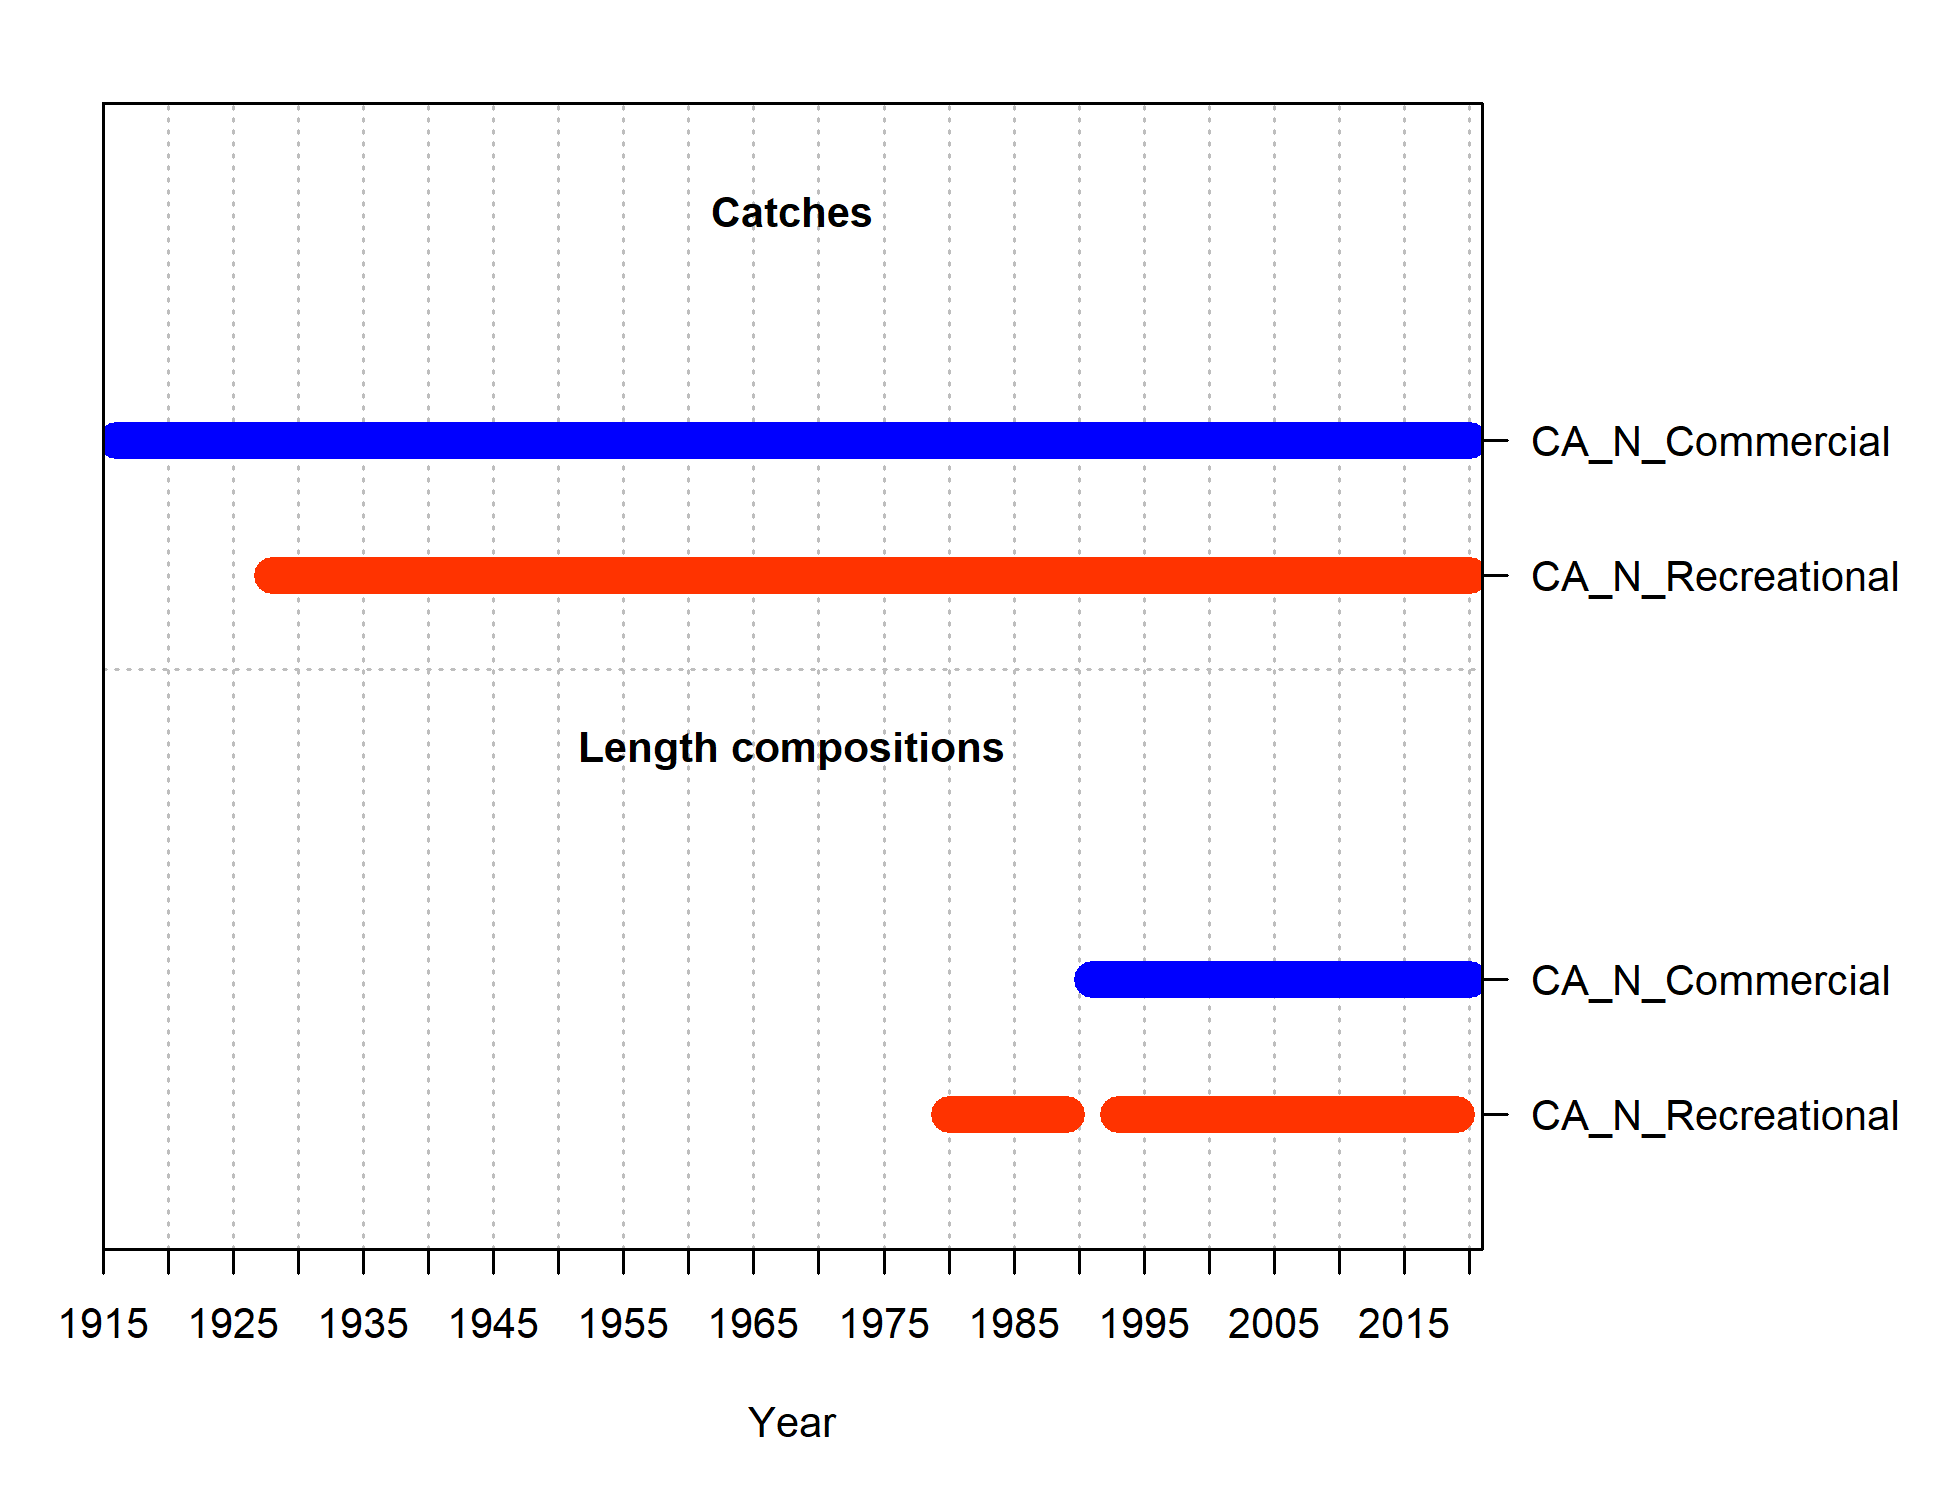
\includegraphics[width=1\textwidth,height=1\textheight]{C:/Assessments/2021/copper_rockfish_2021/models/ca_s_pt_c/12.0_base/plots/data_plot.png}
\caption{Summary of data sources used in the base model.\label{fig:data-plot}}
\end{figure}

\tagmcend\tagstructend

\tagstructbegin{tag=Figure,alttext={Length composition data from the commercial fleet.}}\tagmcbegin{tag=Figure}

\begin{figure}
\centering
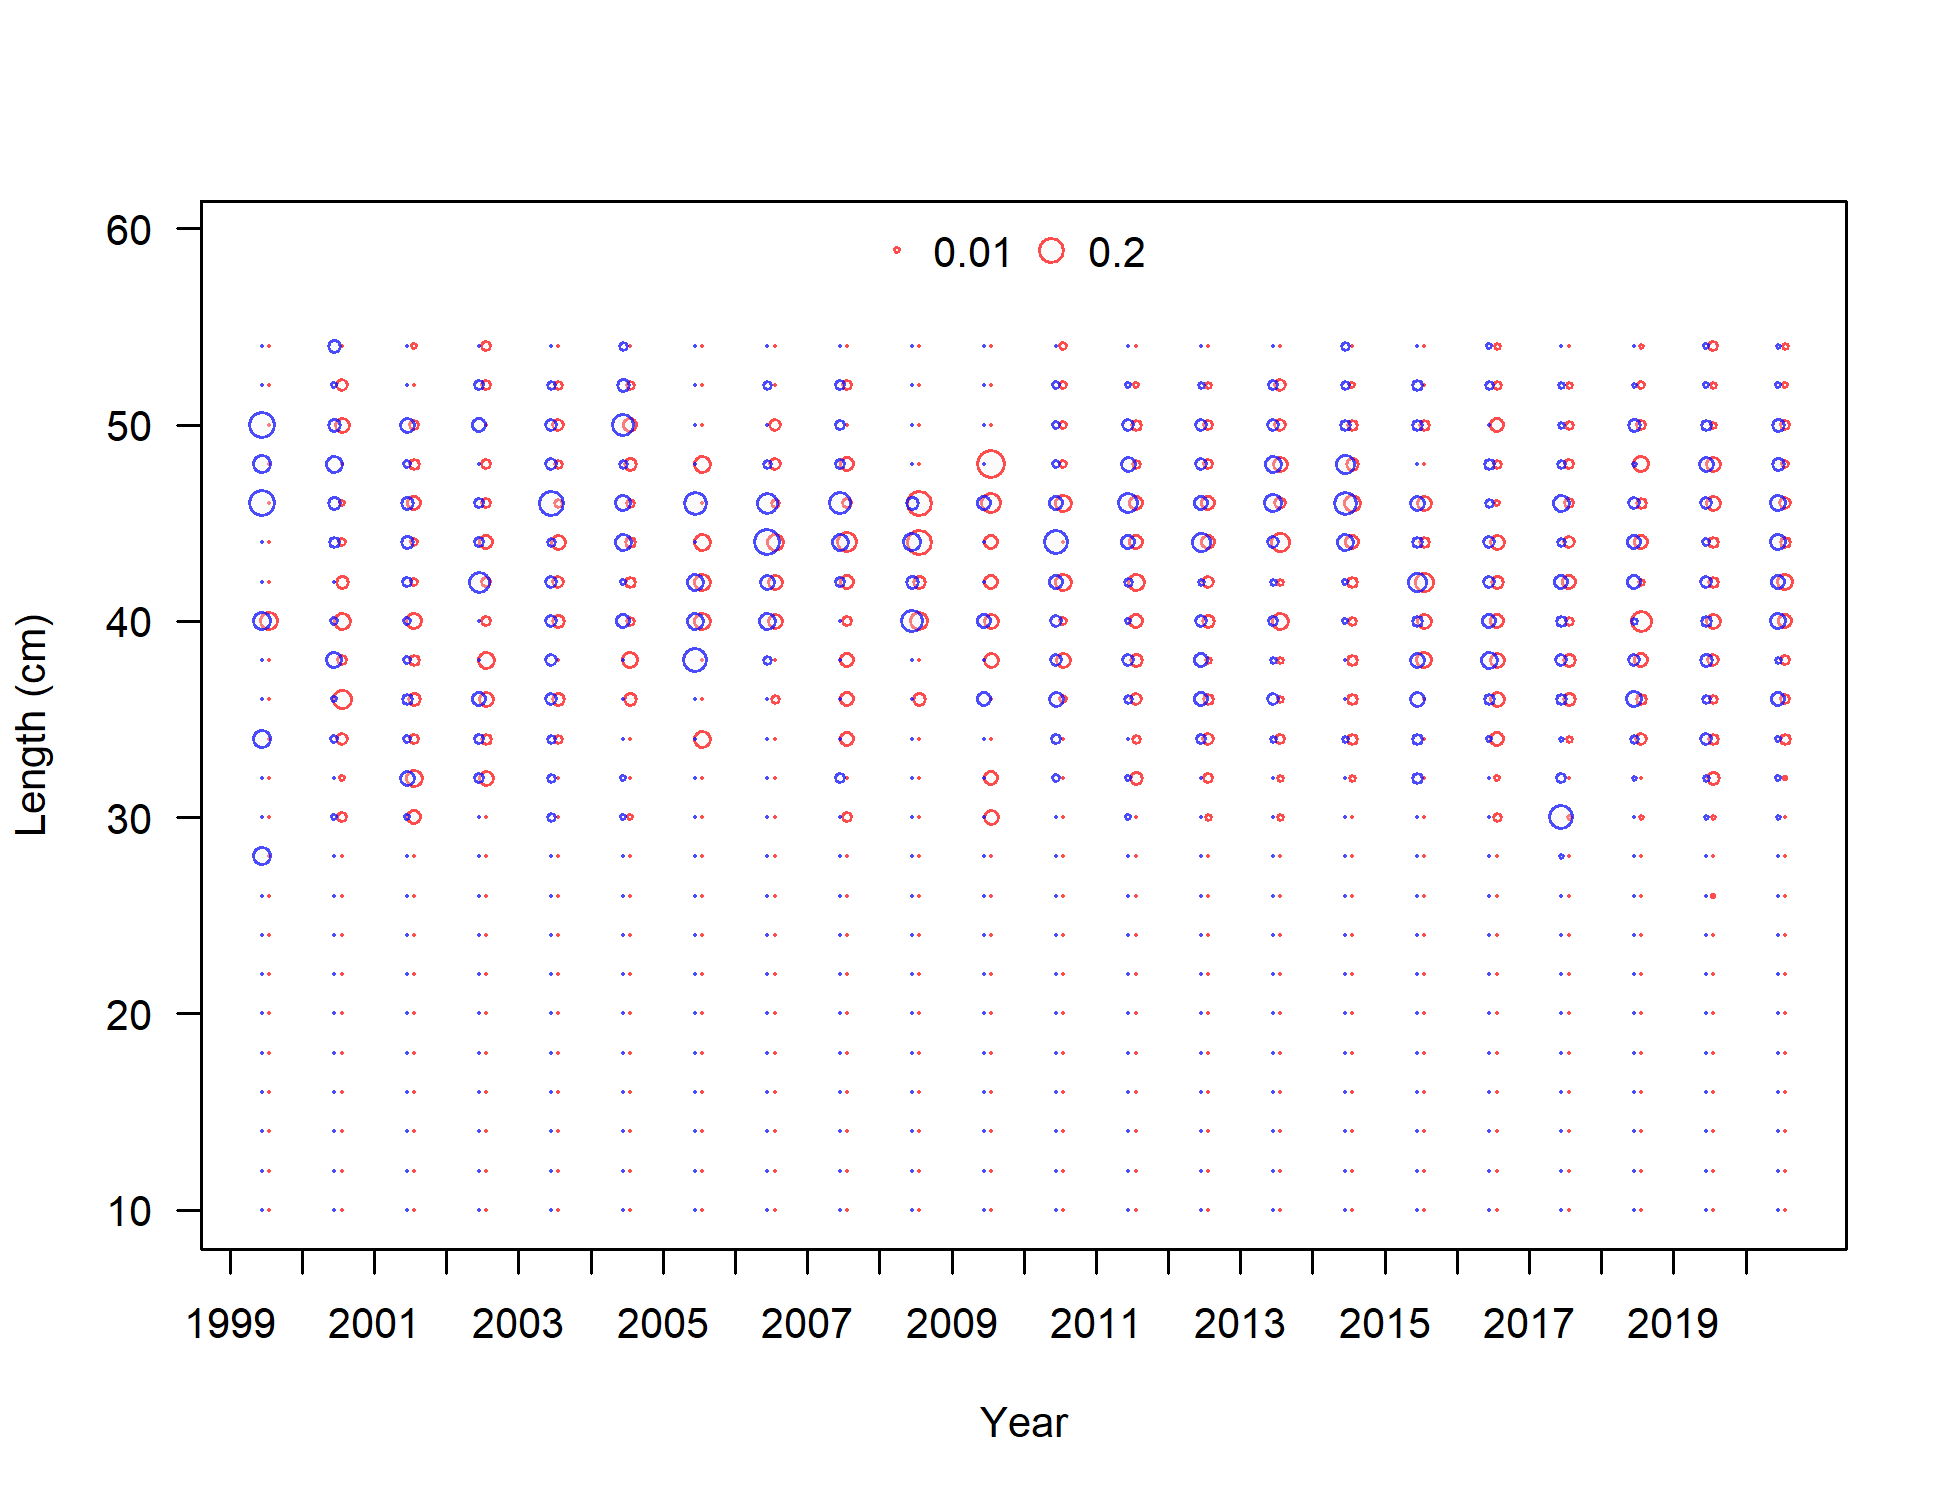
\includegraphics[width=1\textwidth,height=1\textheight]{C:/Assessments/2021/copper_rockfish_2021/models/ca_s_pt_c/12.0_base/plots/comp_lendat_bubflt1mkt0_page2.png}
\caption{Length composition data from the commercial fleet.\label{fig:com-len-data}}
\end{figure}

\tagmcend\tagstructend

\tagstructbegin{tag=Figure,alttext={Mean length for commercial fleet with 95 percent confidence intervals.}}\tagmcbegin{tag=Figure}

\begin{figure}
\centering
\includegraphics[width=1\textwidth,height=1\textheight]{C:/Assessments/2021/copper_rockfish_2021/models/ca_s_pt_c/12.0_base/plots/comp_lendat_data_weighting_TA1.8_CA_S_Commercial.png}
\caption{Mean length for commercial fleet with 95 percent confidence intervals.\label{fig:mean-com-len-data}}
\end{figure}

\tagmcend\tagstructend

\tagstructbegin{tag=Figure,alttext={Length composition data from the recreational fleet.}}\tagmcbegin{tag=Figure}

\begin{figure}
\centering
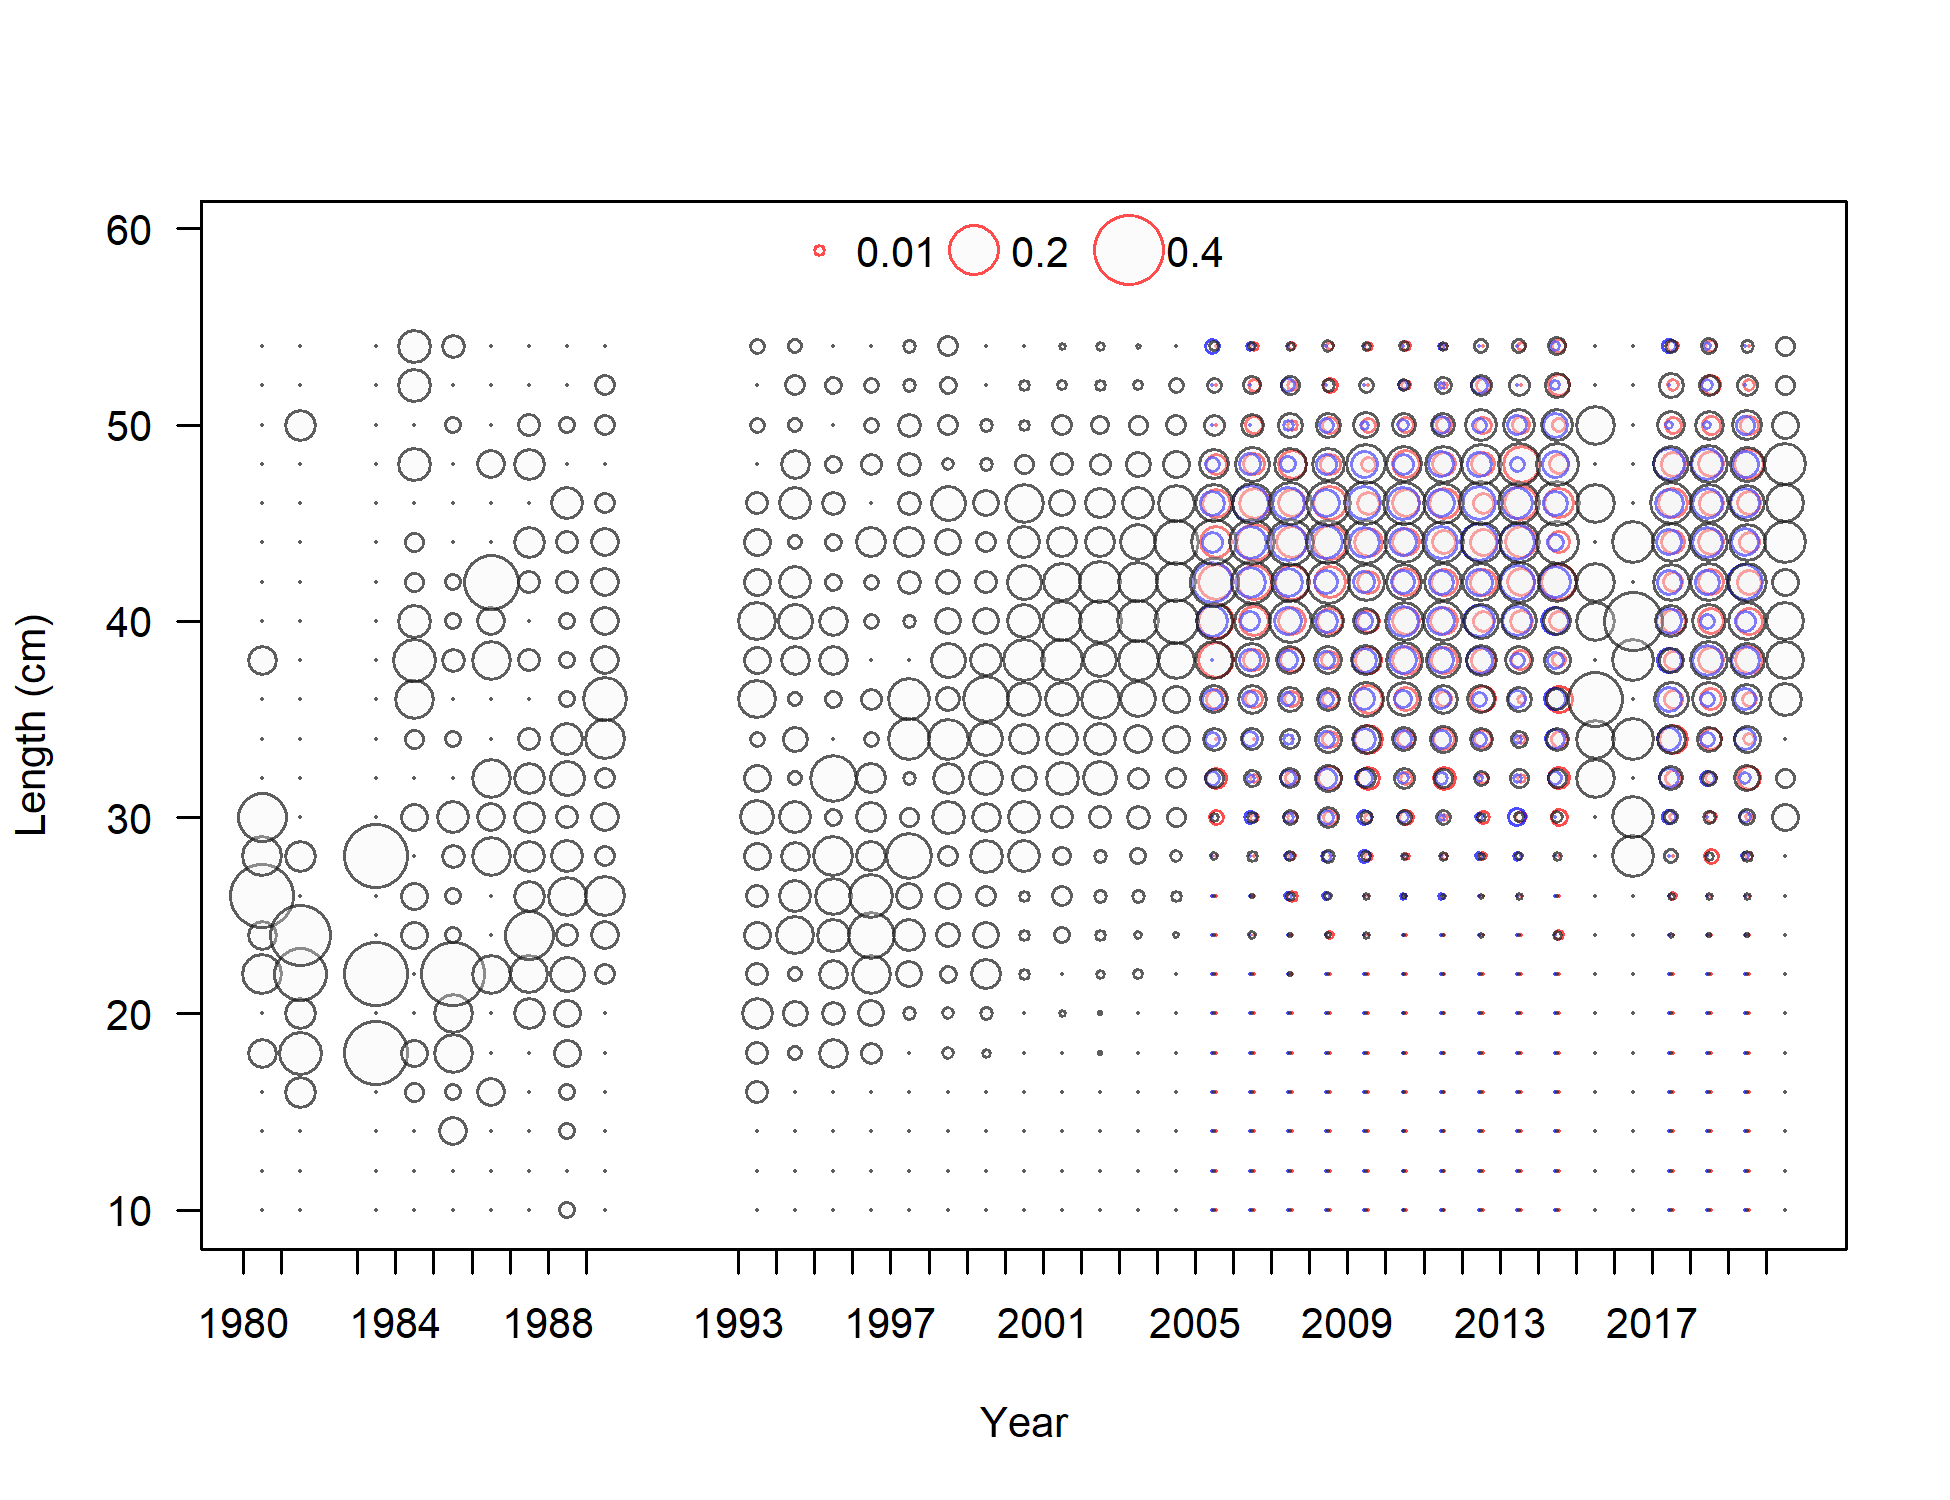
\includegraphics[width=1\textwidth,height=1\textheight]{C:/Assessments/2021/copper_rockfish_2021/models/ca_s_pt_c/12.0_base/plots/comp_lendat_bubflt2mkt0_page3.png}
\caption{Length composition data from the recreational fleet.\label{fig:rec-len-data}}
\end{figure}

\tagmcend\tagstructend

\tagstructbegin{tag=Figure,alttext={Mean length for recreational fleet with 95 percent confidence intervals.}}\tagmcbegin{tag=Figure}

\begin{figure}
\centering
\includegraphics[width=1\textwidth,height=1\textheight]{C:/Assessments/2021/copper_rockfish_2021/models/ca_s_pt_c/12.0_base/plots/comp_lendat_data_weighting_TA1.8_CA_S_Recreational.png}
\caption{Mean length for recreational fleet with 95 percent confidence intervals.\label{fig:mean-rec-len-data}}
\end{figure}

\tagmcend\tagstructend

\tagstructbegin{tag=Figure,alttext={NWFSC Hook and Line sampling sites where yellow sites indicate locations inside Cowcod Conservation Areas.}}\tagmcbegin{tag=Figure}

\begin{figure}
\centering
\includegraphics[width=1\textwidth,height=1\textheight]{//nwcfile/FRAM/Assessments/CurrentAssessments/DataModerate_2021/copper_rockfish/data/survey/plots/HL_SurveyExtent_2017_figure_light_wPorts1024_1.jpg}
\caption{NWFSC Hook and Line sampling sites where yellow sites indicate locations inside Cowcod Conservation Areas.\label{fig:hkl-sites}}
\end{figure}

\tagmcend\tagstructend

\tagstructbegin{tag=Figure,alttext={NWFSC Hook and Line sample sites inside and outside the CCA and site with observations of copper rockfish.}}\tagmcbegin{tag=Figure}

\begin{figure}
\centering
\includegraphics[width=1\textwidth,height=1\textheight]{//nwcfile/FRAM/Assessments/CurrentAssessments/DataModerate_2021/copper_rockfish/data/survey/plots/HKL_Site_Observations.png}
\caption{NWFSC Hook and Line sample sites inside and outside the CCA and site with observations of copper rockfish.\label{fig:hkl-site-ob}}
\end{figure}

\tagmcend\tagstructend

\tagstructbegin{tag=Figure,alttext={NWFSC Hook and Line observations by year outside and inside the cowcod conservation area.}}\tagmcbegin{tag=Figure}

\begin{figure}
\centering
\includegraphics[width=1\textwidth,height=1\textheight]{//nwcfile/FRAM/Assessments/CurrentAssessments/DataModerate_2021/copper_rockfish/data/biology/plots/hkl_cca_comparison.png}
\caption{NWFSC Hook and Line observations by year outside and inside the cowcod conservation area.\label{fig:hkl-cca}}
\end{figure}

\tagmcend\tagstructend

\tagstructbegin{tag=Figure,alttext={Lengths observations by depth in the NWFSC Hook and Line data.}}\tagmcbegin{tag=Figure}

\begin{figure}
\centering
\includegraphics[width=1\textwidth,height=1\textheight]{//nwcfile/FRAM/Assessments/CurrentAssessments/DataModerate_2021/copper_rockfish/data/survey/plots/HKL_Size_by_Depth.png}
\caption{Lengths observations by depth in the NWFSC Hook and Line data.\label{fig:hkl-len-dep}}
\end{figure}

\tagmcend\tagstructend

\tagstructbegin{tag=Figure,alttext={Length composition data from the NWFSC Hook and Line fleet.}}\tagmcbegin{tag=Figure}

\begin{figure}
\centering
\includegraphics[width=1\textwidth,height=1\textheight]{C:/Assessments/2021/copper_rockfish_2021/models/ca_s_pt_c/12.0_base/plots/comp_lendat_bubflt3mkt0.png}
\caption{Length composition data from the NWFSC Hook and Line fleet.\label{fig:hkl-len-data}}
\end{figure}

\tagmcend\tagstructend

\tagstructbegin{tag=Figure,alttext={Mean length for NWFSC Hook and Line fleet with 95 percent confidence intervals.}}\tagmcbegin{tag=Figure}

\begin{figure}
\centering
\includegraphics[width=1\textwidth,height=1\textheight]{C:/Assessments/2021/copper_rockfish_2021/models/ca_s_pt_c/12.0_base/plots/comp_lendat_data_weighting_TA1.8_NWFSC_HKL.png}
\caption{Mean length for NWFSC Hook and Line fleet with 95 percent confidence intervals.\label{fig:mean-hkl-len-data}}
\end{figure}

\tagmcend\tagstructend

\tagstructbegin{tag=Figure,alttext={Index of abundance for the NWFSC Hook and Line survey. Lines indicate 95 percent uncertainty interval around index values based on the model assumption of lognormal error. Thicker lines indicate input uncertainty before addition of estimated additional uncertainty parameter.}}\tagmcbegin{tag=Figure}

\begin{figure}
\centering
\includegraphics[width=1\textwidth,height=1\textheight]{C:/Assessments/2021/copper_rockfish_2021/models/ca_s_pt_c/12.0_base/plots/index1_cpuedata_NWFSC_HKL.png}
\caption{Index of abundance for the NWFSC Hook and Line survey. Lines indicate 95 percent uncertainty interval around index values based on the model assumption of lognormal error. Thicker lines indicate input uncertainty before addition of estimated additional uncertainty parameter.\label{fig:hkl-index}}
\end{figure}

\tagmcend\tagstructend

\tagstructbegin{tag=Figure,alttext={Diangostics for the binomial generalized-linear model.}}\tagmcbegin{tag=Figure}

\begin{figure}
\centering
\includegraphics[width=1\textwidth,height=1\textheight]{//nwcfile/FRAM/Assessments/CurrentAssessments/DataModerate_2021/copper_rockfish/data/survey_indices/Copp.2019.NFT.1m.ALL/Copp.ALL.GAM.Fig.png}
\caption{Diangostics for the binomial generalized-linear model.\label{fig:hkl-diag}}
\end{figure}

\tagmcend\tagstructend

\tagstructbegin{tag=Figure,alttext={Count of length observations across depths in an open access area.}}\tagmcbegin{tag=Figure}

\begin{figure}
\centering
\includegraphics[width=1\textwidth,height=1\textheight]{//nwcfile/FRAM/Assessments/CurrentAssessments/DataModerate_2021/copper_rockfish/data/survey/rov/copper_socal_open_area.png}
\caption{Count of length observations across depths in an open access area.\label{fig:rov-open}}
\end{figure}

\tagmcend\tagstructend

\tagstructbegin{tag=Figure,alttext={Count of length observations across depths within a marine protected area.}}\tagmcbegin{tag=Figure}

\begin{figure}
\centering
\includegraphics[width=1\textwidth,height=1\textheight]{//nwcfile/FRAM/Assessments/CurrentAssessments/DataModerate_2021/copper_rockfish/data/survey/rov/copper_socal_mpa_area.png}
\caption{Count of length observations across depths within a marine protected area.\label{fig:rov-mpa}}
\end{figure}

\tagmcend\tagstructend

\tagstructbegin{tag=Figure,alttext={Comparison of the length-at-weight data from the NWFSC Hook and Line and the NWFSC WCGBT surveys.}}\tagmcbegin{tag=Figure}

\begin{figure}
\centering
\includegraphics[width=1\textwidth,height=1\textheight]{//nwcfile/FRAM/Assessments/CurrentAssessments/DataModerate_2021/copper_rockfish/data/biology/plots/doc_Length_Weight_Source.png}
\caption{Comparison of the length-at-weight data from the NWFSC Hook and Line and the NWFSC WCGBT surveys.\label{fig:len-weight-survey}}
\end{figure}

\tagmcend\tagstructend

\tagstructbegin{tag=Figure,alttext={Survey length-at-weight data with sex specific estimated fits.}}\tagmcbegin{tag=Figure}

\begin{figure}
\centering
\includegraphics[width=1\textwidth,height=1\textheight]{//nwcfile/FRAM/Assessments/CurrentAssessments/DataModerate_2021/copper_rockfish/data/biology/plots/doc_Length_Weight_Sex.png}
\caption{Survey length-at-weight data with sex specific estimated fits.\label{fig:len-weight}}
\end{figure}

\tagmcend\tagstructend

\tagstructbegin{tag=Figure,alttext={Length-at-age for non-randomly sampled larger fish observed by the NWFSC Hook and Line and WCGBT survey.}}\tagmcbegin{tag=Figure}

\begin{figure}
\centering
\includegraphics[width=1\textwidth,height=1\textheight]{//nwcfile/FRAM/Assessments/CurrentAssessments/DataModerate_2021/copper_rockfish/data/biology/plots/South_Len_at_Age.png}
\caption{Length-at-age for non-randomly sampled larger fish observed by the NWFSC Hook and Line and WCGBT survey.\label{fig:survey-len-at-age-data}}
\end{figure}

\tagmcend\tagstructend

\tagstructbegin{tag=Figure,alttext={Length-at-age for non-randomly sampled larger fish observed by the NWFSC Hook and Line and WCGBT survey and young fish from Lea.}}\tagmcbegin{tag=Figure}

\begin{figure}
\centering
\includegraphics[width=1\textwidth,height=1\textheight]{//nwcfile/FRAM/Assessments/CurrentAssessments/DataModerate_2021/copper_rockfish/data/biology/plots/doc_south_Age_by_Sex_Source.png}
\caption{Length-at-age for non-randomly sampled larger fish observed by the NWFSC Hook and Line and WCGBT survey and young fish from Lea.\label{fig:south-len-at-age-data}}
\end{figure}

\tagmcend\tagstructend

\tagstructbegin{tag=Figure,alttext={Length-at-age comparisons between survey collected fish south of Pt. Conception and to those observed off the coast of Oregon and Washington.}}\tagmcbegin{tag=Figure}

\begin{figure}
\centering
\includegraphics[width=1\textwidth,height=1\textheight]{//nwcfile/FRAM/Assessments/CurrentAssessments/DataModerate_2021/copper_rockfish/data/biology/plots/South_Data_Comparison_Len_at_Age.png}
\caption{Length-at-age comparisons between survey collected fish south of Pt. Conception and to those observed off the coast of Oregon and Washington.\label{fig:len-at-age-comp}}
\end{figure}

\tagmcend\tagstructend

\newpage

\tagstructbegin{tag=Figure,alttext={Length-at-age in the beginning of the year with the coefficient of variation by age within the model.}}\tagmcbegin{tag=Figure}

\begin{figure}
\centering
\includegraphics[width=1\textwidth,height=1\textheight]{C:/Assessments/2021/copper_rockfish_2021/models/ca_s_pt_c/12.0_base/plots/bio1_sizeatage.png}
\caption{Length-at-age in the beginning of the year with the coefficient of variation by age within the model.\label{fig:len-age-ss}}
\end{figure}

\tagmcend\tagstructend

\tagstructbegin{tag=Figure,alttext={Maturity as a function of  length.}}\tagmcbegin{tag=Figure}

\begin{figure}
\centering
\includegraphics[width=1\textwidth,height=1\textheight]{C:/Assessments/2021/copper_rockfish_2021/models/ca_s_pt_c/12.0_base/plots/bio6_maturity.png}
\caption{Maturity as a function of length.\label{fig:maturity}}
\end{figure}

\tagmcend\tagstructend

\tagstructbegin{tag=Figure,alttext={Fecundity as a function of length.}}\tagmcbegin{tag=Figure}

\begin{figure}
\centering
\includegraphics[width=1\textwidth,height=1\textheight]{C:/Assessments/2021/copper_rockfish_2021/models/ca_s_pt_c/12.0_base/plots/bio9_fecundity_len.png}
\caption{Fecundity as a function of length.\label{fig:fecundity}}
\end{figure}

\tagmcend\tagstructend

\tagstructbegin{tag=Figure,alttext={Fraction female by length across all available data sources.}}\tagmcbegin{tag=Figure}

\begin{figure}
\centering
\includegraphics[width=1\textwidth,height=1\textheight]{//nwcfile/FRAM/Assessments/CurrentAssessments/DataModerate_2021/copper_rockfish/data/biology/plots/Length_fraction_female.png}
\caption{Fraction female by length across all available data sources.\label{fig:len-sex-ratio}}
\end{figure}

\tagmcend\tagstructend

\tagstructbegin{tag=Figure,alttext={Fraction female by age across all available data sources.}}\tagmcbegin{tag=Figure}

\begin{figure}
\centering
\includegraphics[width=1\textwidth,height=1\textheight]{//nwcfile/FRAM/Assessments/CurrentAssessments/DataModerate_2021/copper_rockfish/data/biology/plots/Age_fraction_female.png}
\caption{Fraction female by age across all available data sources.\label{fig:age-sex-ratio}}
\end{figure}

\tagmcend\tagstructend

\tagstructbegin{tag=Figure,alttext={Comparison between SS bridge model and the results from the 2013 XDB-SRA model.}}\tagmcbegin{tag=Figure}

\begin{figure}
\centering
\includegraphics[width=1\textwidth,height=1\textheight]{C:/Assessments/2021/copper_rockfish_2021/models/ca_s_pt_c/_bridge/_plots/Initial_Bridge.png}
\caption{Comparison between SS bridge model and the results from the 2013 XDB-SRA model.\label{fig:bridge-1}}
\end{figure}

\tagmcend\tagstructend

\tagstructbegin{tag=Figure,alttext={Adjustment to SS female weight-at-length curve to create a match in stock scale to XDB-SRA.}}\tagmcbegin{tag=Figure}

\begin{figure}
\centering
\includegraphics[width=1\textwidth,height=1\textheight]{C:/Assessments/2021/copper_rockfish_2021/models/ca_s_pt_c/_bridge/_plots/Growth.png}
\caption{Adjustment to SS female weight-at-length curve to create a match in stock scale to XDB-SRA.\label{fig:bridge-growth}}
\end{figure}

\tagmcend\tagstructend

\tagstructbegin{tag=Figure,alttext={The time series of spawning biomass (or output) for updates to the 2013 model.}}\tagmcbegin{tag=Figure}

\begin{figure}
\centering
\includegraphics[width=1\textwidth,height=1\textheight]{C:/Assessments/2021/copper_rockfish_2021/models/ca_s_pt_c/_bridge/_plots/1_bridge_all_compare1_spawnbio.png}
\caption{The time series of spawning biomass (or output) for updates to the 2013 model.\label{fig:bridge-ssb}}
\end{figure}

\tagmcend\tagstructend

\tagstructbegin{tag=Figure,alttext={The time series of fraction unfished for updates to the 2013 model.}}\tagmcbegin{tag=Figure}

\begin{figure}
\centering
\includegraphics[width=1\textwidth,height=1\textheight]{C:/Assessments/2021/copper_rockfish_2021/models/ca_s_pt_c/_bridge/_plots/1_bridge_all_compare3_Bratio.png}
\caption{The time series of fraction unfished for updates to the 2013 model.\label{fig:bridge-depl}}
\end{figure}

\tagmcend\tagstructend

\tagstructbegin{tag=Figure,alttext={The time series of spawning output for the subset of bridge models with the updated fecundity relationship.}}\tagmcbegin{tag=Figure}

\begin{figure}
\centering
\includegraphics[width=1\textwidth,height=1\textheight]{C:/Assessments/2021/copper_rockfish_2021/models/ca_s_pt_c/_bridge/_plots/1_bridge_subset_compare1_spawnbio.png}
\caption{The time series of spawning output for the subset of bridge models with the updated fecundity relationship.\label{fig:bridge-ssb-2}}
\end{figure}

\tagmcend\tagstructend

\tagstructbegin{tag=Figure,alttext={Selectivity at length by fleet.}}\tagmcbegin{tag=Figure}

\begin{figure}
\centering
\includegraphics[width=1\textwidth,height=1\textheight]{C:/Assessments/2021/copper_rockfish_2021/models/ca_s_pt_c/12.0_base/plots/sel01_multiple_fleets_length1.png}
\caption{Selectivity at length by fleet.\label{fig:selex}}
\end{figure}

\tagmcend\tagstructend

\tagstructbegin{tag=Figure,alttext={Estimated time series of age-0 recruits (1000s).}}\tagmcbegin{tag=Figure}

\begin{figure}
\centering
\includegraphics[width=1\textwidth,height=1\textheight]{C:/Assessments/2021/copper_rockfish_2021/models/ca_s_pt_c/12.0_base/plots/ts11_Age-0_recruits_(1000s)_with_95_asymptotic_intervals.png}
\caption{Estimated time series of age-0 recruits (1000s).\label{fig:recruits}}
\end{figure}

\tagmcend\tagstructend

\tagstructbegin{tag=Figure,alttext={Stock-recruit curve. Point colors indicate year, with warmer colors indicating earlier years and cooler colors in showing later years.}}\tagmcbegin{tag=Figure}

\begin{figure}
\centering
\includegraphics[width=1\textwidth,height=1\textheight]{C:/Assessments/2021/copper_rockfish_2021/models/ca_s_pt_c/12.0_base/plots/SR_curve.png}
\caption{Stock-recruit curve. Point colors indicate year, with warmer colors indicating earlier years and cooler colors in showing later years.\label{fig:bh-curve}}
\end{figure}

\tagmcend\tagstructend

\tagstructbegin{tag=Figure,alttext={Pearson residuals for commercial fleet. Closed bubble are positive residuals (observed > expected) and open bubbles are negative residuals (observed < expected).}}\tagmcbegin{tag=Figure}

\begin{figure}
\centering
\includegraphics[width=1\textwidth,height=1\textheight]{C:/Assessments/2021/copper_rockfish_2021/models/ca_s_pt_c/12.0_base/plots/comp_lenfit_residsflt1mkt0_page2.png}
\caption{Pearson residuals for commercial fleet. Closed bubble are positive residuals (observed \textgreater{} expected) and open bubbles are negative residuals (observed \textless{} expected).\label{fig:com-pearson}}
\end{figure}

\tagmcend\tagstructend

\tagstructbegin{tag=Figure,alttext={Mean length for commercial lengths with 95 percent confidence intervals based on current samples sizes.}}\tagmcbegin{tag=Figure}

\begin{figure}
\centering
\includegraphics[width=1\textwidth,height=1\textheight]{C:/Assessments/2021/copper_rockfish_2021/models/ca_s_pt_c/12.0_base/plots/comp_lenfit_data_weighting_TA1.8_CA_S_Commercial.png}
\caption{Mean length for commercial lengths with 95 percent confidence intervals based on current samples sizes.\label{fig:com-mean-len-fit}}
\end{figure}

\tagmcend\tagstructend

\tagstructbegin{tag=Figure,alttext={Pearson residuals for recreational fleet. Closed bubble are positive residuals (observed > expected) and open bubbles are negative residuals (observed < expected).}}\tagmcbegin{tag=Figure}

\begin{figure}
\centering
\includegraphics[width=1\textwidth,height=1\textheight]{C:/Assessments/2021/copper_rockfish_2021/models/ca_s_pt_c/12.0_base/plots/comp_lenfit_residsflt2mkt0_page3.png}
\caption{Pearson residuals for recreational fleet. Closed bubble are positive residuals (observed \textgreater{} expected) and open bubbles are negative residuals (observed \textless{} expected).\label{fig:rec-pearson}}
\end{figure}

\tagmcend\tagstructend

\tagstructbegin{tag=Figure,alttext={Mean length for recreational lengths with 95 percent confidence intervals based on current samples sizes.}}\tagmcbegin{tag=Figure}

\begin{figure}
\centering
\includegraphics[width=1\textwidth,height=1\textheight]{C:/Assessments/2021/copper_rockfish_2021/models/ca_s_pt_c/12.0_base/plots/comp_lenfit_data_weighting_TA1.8_CA_S_Recreational.png}
\caption{Mean length for recreational lengths with 95 percent confidence intervals based on current samples sizes.\label{fig:rec-mean-len-fit}}
\end{figure}

\tagmcend\tagstructend

\tagstructbegin{tag=Figure,alttext={Pearson residuals for NWFSC Hook and Line survey. Closed bubble are positive residuals (observed > expected) and open bubbles are negative residuals (observed < expected).}}\tagmcbegin{tag=Figure}

\begin{figure}
\centering
\includegraphics[width=1\textwidth,height=1\textheight]{C:/Assessments/2021/copper_rockfish_2021/models/ca_s_pt_c/12.0_base/plots/comp_lenfit_residsflt3mkt0.png}
\caption{Pearson residuals for NWFSC Hook and Line survey. Closed bubble are positive residuals (observed \textgreater{} expected) and open bubbles are negative residuals (observed \textless{} expected).\label{fig:hkl-pearson}}
\end{figure}

\tagmcend\tagstructend

\tagstructbegin{tag=Figure,alttext={Mean length for recreational lengths with 95 percent confidence intervals based on current samples sizes.}}\tagmcbegin{tag=Figure}

\begin{figure}
\centering
\includegraphics[width=1\textwidth,height=1\textheight]{C:/Assessments/2021/copper_rockfish_2021/models/ca_s_pt_c/12.0_base/plots/comp_lenfit_data_weighting_TA1.8_NWFSC_HKL.png}
\caption{Mean length for recreational lengths with 95 percent confidence intervals based on current samples sizes.\label{fig:hkl-mean-len-fit}}
\end{figure}

\tagmcend\tagstructend

\tagstructbegin{tag=Figure,alttext={Aggregated length comps over all years.}}\tagmcbegin{tag=Figure}

\begin{figure}
\centering
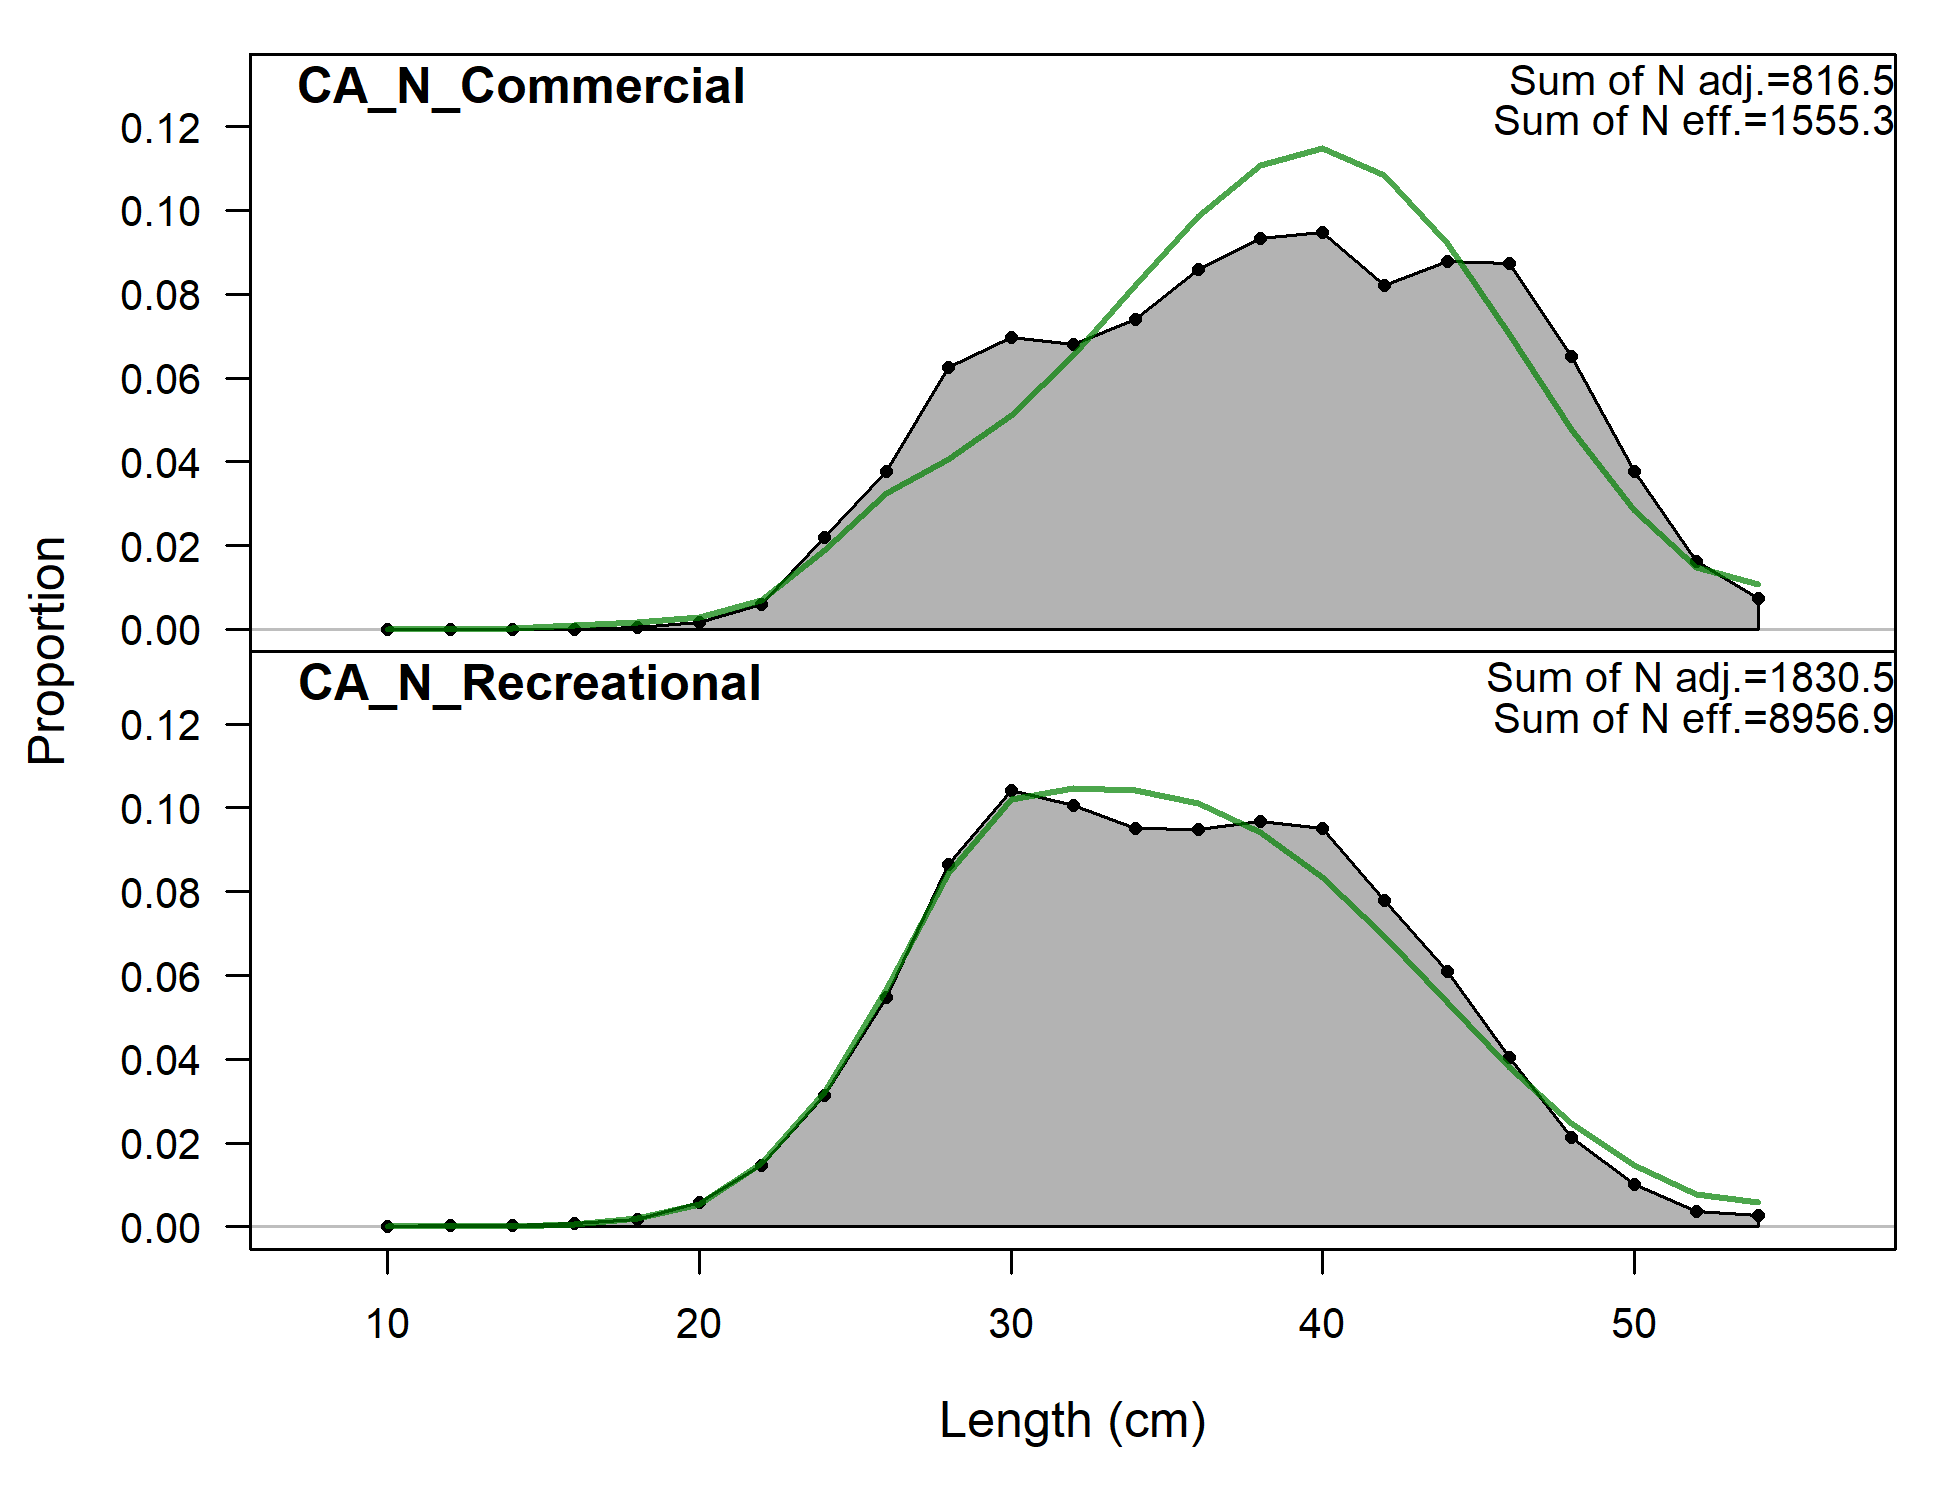
\includegraphics[width=1\textwidth,height=1\textheight]{C:/Assessments/2021/copper_rockfish_2021/models/ca_s_pt_c/12.0_base/plots/comp_lenfit__aggregated_across_time.png}
\caption{Aggregated length comps over all years.\label{fig:agg-len-fit}}
\end{figure}

\tagmcend\tagstructend

\tagstructbegin{tag=Figure,alttext={Fit to index data for the NWFSC Hook and Line survey.}}\tagmcbegin{tag=Figure}

\begin{figure}
\centering
\includegraphics[width=1\textwidth,height=1\textheight]{C:/Assessments/2021/copper_rockfish_2021/models/ca_s_pt_c/12.0_base/plots/index2_cpuefit_NWFSC_HKL.png}
\caption{Fit to index data for the NWFSC Hook and Line survey.\label{fig:index-fit}}
\end{figure}

\tagmcend\tagstructend

\tagstructbegin{tag=Figure,alttext={Estimated time series of spawning output.}}\tagmcbegin{tag=Figure}

\begin{figure}
\centering
\includegraphics[width=1\textwidth,height=1\textheight]{C:/Assessments/2021/copper_rockfish_2021/models/ca_s_pt_c/12.0_base/plots/ts7_Spawning_output_with_95_asymptotic_intervals_intervals.png}
\caption{Estimated time series of spawning output.\label{fig:ssb}}
\end{figure}

\tagmcend\tagstructend

\tagstructbegin{tag=Figure,alttext={Estimated time series of total biomass.}}\tagmcbegin{tag=Figure}

\begin{figure}
\centering
\includegraphics[width=1\textwidth,height=1\textheight]{C:/Assessments/2021/copper_rockfish_2021/models/ca_s_pt_c/12.0_base/plots/ts1_Total_biomass_(mt).png}
\caption{Estimated time series of total biomass.\label{fig:tot-bio}}
\end{figure}

\tagmcend\tagstructend

\tagstructbegin{tag=Figure,alttext={Estimated time series of fraction of unfished spawning output.}}\tagmcbegin{tag=Figure}

\begin{figure}
\centering
\includegraphics[width=1\textwidth,height=1\textheight]{C:/Assessments/2021/copper_rockfish_2021/models/ca_s_pt_c/12.0_base/plots/ts9_Relative_spawning_output_intervals.png}
\caption{Estimated time series of fraction of unfished spawning output.\label{fig:depl}}
\end{figure}

\tagmcend\tagstructend

\tagstructbegin{tag=Figure,alttext={Estimated 1 - relative spawning ratio (SPR) by year.}}\tagmcbegin{tag=Figure}

\begin{figure}
\centering
\includegraphics[width=1\textwidth,height=1\textheight]{C:/Assessments/2021/copper_rockfish_2021/models/ca_s_pt_c/12.0_base/plots/SPR2_minusSPRseries.png}
\caption{Estimated 1 - relative spawning ratio (SPR) by year.\label{fig:1-spr}}
\end{figure}

\tagmcend\tagstructend

\tagstructbegin{tag=Figure,alttext={Equilibrium yield curve for the base case model. Values are based on the 2020 fishery selectivity and with steepness fixed at 0.72.}}\tagmcbegin{tag=Figure}

\begin{figure}
\centering
\includegraphics[width=1\textwidth,height=1\textheight]{C:/Assessments/2021/copper_rockfish_2021/models/ca_s_pt_c/12.0_base/plots/yield2_yield_curve_with_refpoints.png}
\caption{Equilibrium yield curve for the base case model. Values are based on the 2020 fishery selectivity and with steepness fixed at 0.72.\label{fig:yield}}
\end{figure}

\tagmcend\tagstructend

\tagstructbegin{tag=Figure,alttext={Change in estimated spawning output by sensitivity.}}\tagmcbegin{tag=Figure}

\begin{figure}
\centering
\includegraphics[width=1\textwidth,height=1\textheight]{//nwcfile/FRAM/Assessments/CurrentAssessments/DataModerate_2021/copper_rockfish/models/ca_s_pt_c/_sensitivities/_plots/12.0_base_1_compare2_spawnbio_uncertainty.png}
\caption{Change in estimated spawning output by sensitivity.\label{fig:sens-ssb-1}}
\end{figure}

\tagmcend\tagstructend

\tagstructbegin{tag=Figure,alttext={Change in estimated fraction unfished by sensitivity.}}\tagmcbegin{tag=Figure}

\begin{figure}
\centering
\includegraphics[width=1\textwidth,height=1\textheight]{//nwcfile/FRAM/Assessments/CurrentAssessments/DataModerate_2021/copper_rockfish/models/ca_s_pt_c/_sensitivities/_plots/12.0_base_1_compare4_Bratio_uncertainty.png}
\caption{Change in estimated fraction unfished by sensitivity.\label{fig:sens-depl-1}}
\end{figure}

\tagmcend\tagstructend

\tagstructbegin{tag=Figure,alttext={Change in estimated spawning output by sensitivity.}}\tagmcbegin{tag=Figure}

\begin{figure}
\centering
\includegraphics[width=1\textwidth,height=1\textheight]{//nwcfile/FRAM/Assessments/CurrentAssessments/DataModerate_2021/copper_rockfish/models/ca_s_pt_c/_sensitivities/_plots/12.0_base_2_compare2_spawnbio_uncertainty.png}
\caption{Change in estimated spawning output by sensitivity.\label{fig:sens-ssb-2}}
\end{figure}

\tagmcend\tagstructend

\tagstructbegin{tag=Figure,alttext={Change in estimated fraction unfished by sensitivity.}}\tagmcbegin{tag=Figure}

\includegraphics[width=1\textwidth,height=1\textheight]{//nwcfile/FRAM/Assessments/CurrentAssessments/DataModerate_2021/copper_rockfish/models/ca_s_pt_c/_sensitivities/_plots/12.0_base_2_compare4_Bratio_uncertainty.png} \newpage

\tagmcend\tagstructend

\tagstructbegin{tag=Figure,alttext={LB-SPR yearly estimates of selectivity, the ratio of fishing intensity to natural mortality (F/M), and annual spawner-per-recruit (SPR) values.}}\tagmcbegin{tag=Figure}

\begin{figure}
\centering
\includegraphics[width=1\textwidth,height=1\textheight]{C:/Assessments/2021/copper_rockfish_2021/models/lbspr/Copper_SoCAL_YrEsts_newVBGF.png}
\caption{LB-SPR yearly estimates of selectivity, the ratio of fishing intensity to natural mortality (F/M), and annual spawner-per-recruit (SPR) values.\label{fig:lbspr}}
\end{figure}

\tagmcend\tagstructend

\newpage

\tagstructbegin{tag=Figure,alttext={Change in the negative log-likelihood across a range of log(R0) values.}}\tagmcbegin{tag=Figure}

\begin{figure}
\centering
\includegraphics[width=1\textwidth,height=1\textheight]{C:/Assessments/2021/copper_rockfish_2021/models/ca_s_pt_c/12.0_base_profile_SR_LN(R0)/piner_panel_SR_LN(R0).png}
\caption{Change in the negative log-likelihood across a range of log(R0) values.\label{fig:r0-profile}}
\end{figure}

\tagmcend\tagstructend

\tagstructbegin{tag=Figure,alttext={Change in the estimate of spawning output across a range of log(R0) values.}}\tagmcbegin{tag=Figure}

\begin{figure}
\centering
\includegraphics[width=1\textwidth,height=1\textheight]{C:/Assessments/2021/copper_rockfish_2021/models/ca_s_pt_c/12.0_base_profile_SR_LN(R0)/SR_LN(R0)_trajectories_compare1_spawnbio.png}
\caption{Change in the estimate of spawning output across a range of log(R0) values.\label{fig:r0-ssb}}
\end{figure}

\tagmcend\tagstructend

\tagstructbegin{tag=Figure,alttext={Change in the estimate of fraction unfished across a range of log(R0) values.}}\tagmcbegin{tag=Figure}

\begin{figure}
\centering
\includegraphics[width=1\textwidth,height=1\textheight]{C:/Assessments/2021/copper_rockfish_2021/models/ca_s_pt_c/12.0_base_profile_SR_LN(R0)/SR_LN(R0)_trajectories_compare3_Bratio.png}
\caption{Change in the estimate of fraction unfished across a range of log(R0) values.\label{fig:r0-depl}}
\end{figure}

\tagmcend\tagstructend

\tagstructbegin{tag=Figure,alttext={Change in the negative log-likelihood across a range of steepness values.}}\tagmcbegin{tag=Figure}

\begin{figure}
\centering
\includegraphics[width=1\textwidth,height=1\textheight]{C:/Assessments/2021/copper_rockfish_2021/models/ca_s_pt_c/12.0_base_profile_SR_BH_steep/piner_panel_SR_BH_steep.png}
\caption{Change in the negative log-likelihood across a range of steepness values.\label{fig:h-profile}}
\end{figure}

\tagmcend\tagstructend

\tagstructbegin{tag=Figure,alttext={Change in the estimate of spawning output across a range of steepness values.}}\tagmcbegin{tag=Figure}

\begin{figure}
\centering
\includegraphics[width=1\textwidth,height=1\textheight]{C:/Assessments/2021/copper_rockfish_2021/models/ca_s_pt_c/12.0_base_profile_SR_BH_steep/SR_BH_steep_trajectories_compare1_spawnbio.png}
\caption{Change in the estimate of spawning output across a range of steepness values.\label{fig:h-ssb}}
\end{figure}

\tagmcend\tagstructend

\tagstructbegin{tag=Figure,alttext={Change in the estimate of fraction unfished across a range of steepness values.}}\tagmcbegin{tag=Figure}

\begin{figure}
\centering
\includegraphics[width=1\textwidth,height=1\textheight]{C:/Assessments/2021/copper_rockfish_2021/models/ca_s_pt_c/12.0_base_profile_SR_BH_steep/SR_BH_steep_trajectories_compare3_Bratio.png}
\caption{Change in the estimate of fraction unfished across a range of steepness values.\label{fig:h-depl}}
\end{figure}

\tagmcend\tagstructend

\tagstructbegin{tag=Figure,alttext={Change in the negative log-likelihood across a range of female natural mortality values.}}\tagmcbegin{tag=Figure}

\begin{figure}
\centering
\includegraphics[width=1\textwidth,height=1\textheight]{C:/Assessments/2021/copper_rockfish_2021/models/ca_s_pt_c/12.0_base_profile_NatM_p_1_Fem_GP_1/piner_panel_NatM_p_1_Fem_GP_1.png}
\caption{Change in the negative log-likelihood across a range of female natural mortality values.\label{fig:m-profile}}
\end{figure}

\tagmcend\tagstructend

\tagstructbegin{tag=Figure,alttext={Change in the estimate of spawning output across a range of female natural mortality values.}}\tagmcbegin{tag=Figure}

\begin{figure}
\centering
\includegraphics[width=1\textwidth,height=1\textheight]{C:/Assessments/2021/copper_rockfish_2021/models/ca_s_pt_c/12.0_base_profile_NatM_p_1_Fem_GP_1/NatM_p_1_Fem_GP_1_trajectories_compare1_spawnbio.png}
\caption{Change in the estimate of spawning output across a range of female natural mortality values.\label{fig:m-ssb}}
\end{figure}

\tagmcend\tagstructend

\tagstructbegin{tag=Figure,alttext={Change in the estimate of fraction unfished across a range of female natural values.}}\tagmcbegin{tag=Figure}

\begin{figure}
\centering
\includegraphics[width=1\textwidth,height=1\textheight]{C:/Assessments/2021/copper_rockfish_2021/models/ca_s_pt_c/12.0_base_profile_NatM_p_1_Fem_GP_1/NatM_p_1_Fem_GP_1_trajectories_compare3_Bratio.png}
\caption{Change in the estimate of fraction unfished across a range of female natural values.\label{fig:m-depl}}
\end{figure}

\tagmcend\tagstructend

\tagstructbegin{tag=Figure,alttext={Change in the negative log-likelihood across a range of female maximum length values.}}\tagmcbegin{tag=Figure}

\begin{figure}
\centering
\includegraphics[width=1\textwidth,height=1\textheight]{C:/Assessments/2021/copper_rockfish_2021/models/ca_s_pt_c/12.0_base_profile_L_at_Amax_Fem_GP_1/piner_panel_L_at_Amax_Fem_GP_1.png}
\caption{Change in the negative log-likelihood across a range of female maximum length values.\label{fig:linf-profile}}
\end{figure}

\tagmcend\tagstructend

\tagstructbegin{tag=Figure,alttext={Change in the estimate of spawning output across a range of female maximum length values.}}\tagmcbegin{tag=Figure}

\begin{figure}
\centering
\includegraphics[width=1\textwidth,height=1\textheight]{C:/Assessments/2021/copper_rockfish_2021/models/ca_s_pt_c/12.0_base_profile_L_at_Amax_Fem_GP_1/L_at_Amax_Fem_GP_1_trajectories_compare1_spawnbio.png}
\caption{Change in the estimate of spawning output across a range of female maximum length values.\label{fig:linf-ssb}}
\end{figure}

\tagmcend\tagstructend

\tagstructbegin{tag=Figure,alttext={Change in the estimate of fraction unfished across a range of female maximum length values.}}\tagmcbegin{tag=Figure}

\begin{figure}
\centering
\includegraphics[width=1\textwidth,height=1\textheight]{C:/Assessments/2021/copper_rockfish_2021/models/ca_s_pt_c/12.0_base_profile_L_at_Amax_Fem_GP_1/L_at_Amax_Fem_GP_1_trajectories_compare3_Bratio.png}
\caption{Change in the estimate of fraction unfished across a range of female maximum length values.\label{fig:linf-depl}}
\end{figure}

\tagmcend\tagstructend

\tagstructbegin{tag=Figure,alttext={Change in the negative log-likelihood across a range of female k values.}}\tagmcbegin{tag=Figure}

\begin{figure}
\centering
\includegraphics[width=1\textwidth,height=1\textheight]{C:/Assessments/2021/copper_rockfish_2021/models/ca_s_pt_c/12.0_base_profile_VonBert_K_Fem_GP_1/piner_panel_VonBert_K_Fem_GP_1.png}
\caption{Change in the negative log-likelihood across a range of female k values.\label{fig:k-profile}}
\end{figure}

\tagmcend\tagstructend

\tagstructbegin{tag=Figure,alttext={Change in the estimate of spawning output across a range of female k values.}}\tagmcbegin{tag=Figure}

\begin{figure}
\centering
\includegraphics[width=1\textwidth,height=1\textheight]{C:/Assessments/2021/copper_rockfish_2021/models/ca_s_pt_c/12.0_base_profile_VonBert_K_Fem_GP_1/VonBert_K_Fem_GP_1_trajectories_compare1_spawnbio.png}
\caption{Change in the estimate of spawning output across a range of female k values.\label{fig:k-ssb}}
\end{figure}

\tagmcend\tagstructend

\tagstructbegin{tag=Figure,alttext={Change in the estimate of fraction unfished across a range of female k values.}}\tagmcbegin{tag=Figure}

\begin{figure}
\centering
\includegraphics[width=1\textwidth,height=1\textheight]{C:/Assessments/2021/copper_rockfish_2021/models/ca_s_pt_c/12.0_base_profile_VonBert_K_Fem_GP_1/VonBert_K_Fem_GP_1_trajectories_compare3_Bratio.png}
\caption{Change in the estimate of fraction unfished across a range of female k values.\label{fig:k-depl}}
\end{figure}

\tagmcend\tagstructend

\tagstructbegin{tag=Figure,alttext={Change in the estimate of spawning output when the most recent 5 years of data area removed sequentially.}}\tagmcbegin{tag=Figure}

\begin{figure}
\centering
\includegraphics[width=1\textwidth,height=1\textheight]{C:/Assessments/2021/copper_rockfish_2021/models/ca_s_pt_c/12.0_base_retro/compare2_spawnbio_uncertainty.png}
\caption{Change in the estimate of spawning output when the most recent 5 years of data area removed sequentially.\label{fig:retro-ssb}}
\end{figure}

\tagmcend\tagstructend

\tagstructbegin{tag=Figure,alttext={Change in the estimate of fraction unfished when the most recent 5 years of data area removed sequentially.}}\tagmcbegin{tag=Figure}

\begin{figure}
\centering
\includegraphics[width=1\textwidth,height=1\textheight]{C:/Assessments/2021/copper_rockfish_2021/models/ca_s_pt_c/12.0_base_retro/compare4_Bratio_uncertainty.png}
\caption{Change in the estimate of fraction unfished when the most recent 5 years of data area removed sequentially.\label{fig:retro-depl}}
\end{figure}

\tagmcend\tagstructend

\newpage

\clearpage

\tagstructbegin{tag=H1}\tagmcbegin{tag=H1}

\hypertarget{appendix-a}{%
\section{Appendix A}\label{appendix-a}}

\leavevmode\tagmcend\tagstructend

\tagstructbegin{tag=H2}\tagmcbegin{tag=H2}

\hypertarget{annual-length-composition-data}{%
\subsection{Annual Length Composition Data}\label{annual-length-composition-data}}

\leavevmode\tagmcend\tagstructend

\tagstructbegin{tag=Figure,alttext={Length comp data, whole catch, CA_S_Commercial (plot 1 of 2).<br><br>'N adj.' is the input sample size after data-weighting adjustment. N eff. is the calculated effective sample size used in the McAllister-Iannelli tuning method..}}\tagmcbegin{tag=Figure}

\begin{figure}
\centering
\includegraphics[width=1\textwidth,height=1\textheight]{C:/Assessments/2021/copper_rockfish_2021/models/ca_s_pt_c/12.0_base/plots/comp_lendat_flt1mkt0_page1.png}
\caption{Length comp data, whole catch, CA\_S\_Commercial (plot 1 of 2).`N adj.' is the input sample size after data-weighting adjustment. N eff. is the calculated effective sample size used in the McAllister-Iannelli tuning method..\label{fig:comp_lendat_flt1mkt0_page1}}
\end{figure}

\tagmcend\tagstructend

\tagstructbegin{tag=Figure,alttext={Length comp data, whole catch, CA_S_Commercial (plot 2 of 2).}}\tagmcbegin{tag=Figure}

\begin{figure}
\centering
\includegraphics[width=1\textwidth,height=1\textheight]{C:/Assessments/2021/copper_rockfish_2021/models/ca_s_pt_c/12.0_base/plots/comp_lendat_flt1mkt0_page2.png}
\caption{Length comp data, whole catch, CA\_S\_Commercial (plot 2 of 2).\label{fig:comp_lendat_flt1mkt0_page2}}
\end{figure}

\tagmcend\tagstructend

\tagstructbegin{tag=Figure,alttext={Length comp data, whole catch, CA_S_Recreational (plot 1 of 3).<br><br>'N adj.' is the input sample size after data-weighting adjustment. N eff. is the calculated effective sample size used in the McAllister-Iannelli tuning method..}}\tagmcbegin{tag=Figure}

\begin{figure}
\centering
\includegraphics[width=1\textwidth,height=1\textheight]{C:/Assessments/2021/copper_rockfish_2021/models/ca_s_pt_c/12.0_base/plots/comp_lendat_flt2mkt0_page1.png}
\caption{Length comp data, whole catch, CA\_S\_Recreational (plot 1 of 3).`N adj.' is the input sample size after data-weighting adjustment. N eff. is the calculated effective sample size used in the McAllister-Iannelli tuning method..\label{fig:comp_lendat_flt2mkt0_page1}}
\end{figure}

\tagmcend\tagstructend

\tagstructbegin{tag=Figure,alttext={Length comp data, whole catch, CA_S_Recreational (plot 2 of 3).}}\tagmcbegin{tag=Figure}

\begin{figure}
\centering
\includegraphics[width=1\textwidth,height=1\textheight]{C:/Assessments/2021/copper_rockfish_2021/models/ca_s_pt_c/12.0_base/plots/comp_lendat_flt2mkt0_page2.png}
\caption{Length comp data, whole catch, CA\_S\_Recreational (plot 2 of 3).\label{fig:comp_lendat_flt2mkt0_page2}}
\end{figure}

\tagmcend\tagstructend

\tagstructbegin{tag=Figure,alttext={Length comp data, whole catch, CA_S_Recreational (plot 3 of 3).}}\tagmcbegin{tag=Figure}

\begin{figure}
\centering
\includegraphics[width=1\textwidth,height=1\textheight]{C:/Assessments/2021/copper_rockfish_2021/models/ca_s_pt_c/12.0_base/plots/comp_lendat_flt2mkt0_page3.png}
\caption{Length comp data, whole catch, CA\_S\_Recreational (plot 3 of 3).\label{fig:comp_lendat_flt2mkt0_page3}}
\end{figure}

\tagmcend\tagstructend

\tagstructbegin{tag=Figure,alttext={Length comp data, whole catch, NWFSC_HKL.<br><br>'N adj.' is the input sample size after data-weighting adjustment. N eff. is the calculated effective sample size used in the McAllister-Iannelli tuning method..}}\tagmcbegin{tag=Figure}

\begin{figure}
\centering
\includegraphics[width=1\textwidth,height=1\textheight]{C:/Assessments/2021/copper_rockfish_2021/models/ca_s_pt_c/12.0_base/plots/comp_lendat_flt3mkt0.png}
\caption{Length comp data, whole catch, NWFSC\_HKL.`N adj.' is the input sample size after data-weighting adjustment. N eff. is the calculated effective sample size used in the McAllister-Iannelli tuning method..\label{fig:comp_lendat_flt3mkt0}}
\end{figure}

\tagmcend\tagstructend

\newpage

\tagstructbegin{tag=H2}\tagmcbegin{tag=H2}

\hypertarget{detailed-fit-to-length-composition-data}{%
\subsection{Detailed Fit to Length Composition Data}\label{detailed-fit-to-length-composition-data}}

\leavevmode\tagmcend\tagstructend

\tagstructbegin{tag=Figure,alttext={Length comps, whole catch, CA_S_Commercial (plot 1 of 2).<br><br>'N adj.' is the input sample size after data-weighting adjustment. N eff. is the calculated effective sample size used in the McAllister-Iannelli tuning method..}}\tagmcbegin{tag=Figure}

\begin{figure}
\centering
\includegraphics[width=1\textwidth,height=1\textheight]{C:/Assessments/2021/copper_rockfish_2021/models/ca_s_pt_c/12.0_base/plots/comp_lenfit_flt1mkt0_page1.png}
\caption{Length comps, whole catch, CA\_S\_Commercial (plot 1 of 2).`N adj.' is the input sample size after data-weighting adjustment. N eff. is the calculated effective sample size used in the McAllister-Iannelli tuning method..\label{fig:comp_lenfit_flt1mkt0_page1}}
\end{figure}

\tagmcend\tagstructend

\tagstructbegin{tag=Figure,alttext={Length comps, whole catch, CA_S_Commercial (plot 2 of 2).}}\tagmcbegin{tag=Figure}

\begin{figure}
\centering
\includegraphics[width=1\textwidth,height=1\textheight]{C:/Assessments/2021/copper_rockfish_2021/models/ca_s_pt_c/12.0_base/plots/comp_lenfit_flt1mkt0_page2.png}
\caption{Length comps, whole catch, CA\_S\_Commercial (plot 2 of 2).\label{fig:comp_lenfit_flt1mkt0_page2}}
\end{figure}

\tagmcend\tagstructend

\tagstructbegin{tag=Figure,alttext={Length comps, whole catch, CA_S_Recreational (plot 1 of 3).<br><br>'N adj.' is the input sample size after data-weighting adjustment. N eff. is the calculated effective sample size used in the McAllister-Iannelli tuning method..}}\tagmcbegin{tag=Figure}

\begin{figure}
\centering
\includegraphics[width=1\textwidth,height=1\textheight]{C:/Assessments/2021/copper_rockfish_2021/models/ca_s_pt_c/12.0_base/plots/comp_lenfit_flt2mkt0_page1.png}
\caption{Length comps, whole catch, CA\_S\_Recreational (plot 1 of 3).`N adj.' is the input sample size after data-weighting adjustment. N eff. is the calculated effective sample size used in the McAllister-Iannelli tuning method..\label{fig:comp_lenfit_flt2mkt0_page1}}
\end{figure}

\tagmcend\tagstructend

\tagstructbegin{tag=Figure,alttext={Length comps, whole catch, CA_S_Recreational (plot 2 of 3).}}\tagmcbegin{tag=Figure}

\begin{figure}
\centering
\includegraphics[width=1\textwidth,height=1\textheight]{C:/Assessments/2021/copper_rockfish_2021/models/ca_s_pt_c/12.0_base/plots/comp_lenfit_flt2mkt0_page2.png}
\caption{Length comps, whole catch, CA\_S\_Recreational (plot 2 of 3).\label{fig:comp_lenfit_flt2mkt0_page2}}
\end{figure}

\tagmcend\tagstructend

\tagstructbegin{tag=Figure,alttext={Length comps, whole catch, CA_S_Recreational (plot 3 of 3).}}\tagmcbegin{tag=Figure}

\begin{figure}
\centering
\includegraphics[width=1\textwidth,height=1\textheight]{C:/Assessments/2021/copper_rockfish_2021/models/ca_s_pt_c/12.0_base/plots/comp_lenfit_flt2mkt0_page3.png}
\caption{Length comps, whole catch, CA\_S\_Recreational (plot 3 of 3).\label{fig:comp_lenfit_flt2mkt0_page3}}
\end{figure}

\tagmcend\tagstructend

\tagstructbegin{tag=Figure,alttext={Length comps, whole catch, NWFSC_HKL.<br><br>'N adj.' is the input sample size after data-weighting adjustment. N eff. is the calculated effective sample size used in the McAllister-Iannelli tuning method..}}\tagmcbegin{tag=Figure}

\begin{figure}
\centering
\includegraphics[width=1\textwidth,height=1\textheight]{C:/Assessments/2021/copper_rockfish_2021/models/ca_s_pt_c/12.0_base/plots/comp_lenfit_flt3mkt0.png}
\caption{Length comps, whole catch, NWFSC\_HKL.`N adj.' is the input sample size after data-weighting adjustment. N eff. is the calculated effective sample size used in the McAllister-Iannelli tuning method..\label{fig:comp_lenfit_flt3mkt0}}
\end{figure}

\tagmcend\tagstructend

\newpage

\tagstructbegin{tag=H2}\tagmcbegin{tag=H2}

\hypertarget{implied-fit-to-commercial-ghost-fleet-length-data}{%
\subsection{Implied Fit to Commercial `Ghost' Fleet Length Data}\label{implied-fit-to-commercial-ghost-fleet-length-data}}

\leavevmode\tagmcend\tagstructend

\tagstructbegin{tag=Figure,alttext={Ghost length comps, whole catch, CA_S_Commercial.<br><br>'N adj.' is the input sample size after data-weighting adjustment. N eff. is the calculated effective sample size used in the McAllister-Iannelli tuning method..}}\tagmcbegin{tag=Figure}

\begin{figure}
\centering
\includegraphics[width=1\textwidth,height=1\textheight]{C:/Assessments/2021/copper_rockfish_2021/models/ca_s_pt_c/12.0_base/plots/comp_gstlenfit_flt1mkt0.png}
\caption{Ghost length comps, whole catch, CA\_S\_Commercial.`N adj.' is the input sample size after data-weighting adjustment. N eff. is the calculated effective sample size used in the McAllister-Iannelli tuning method..\label{fig:comp_gstlenfit_flt1mkt0}}
\end{figure}

\tagmcend\tagstructend
\end{document}
